\RequirePackage[l2tabu, orthodox]{nag}
% vim: set spell spelllang=fr:
\documentclass[oneside,parskip,draft]{scrbook}

\usepackage[T1]{fontenc}
\usepackage[utf8]{inputenc}
\usepackage{mathptmx}

% no dot after parts
% http://tex.stackexchange.com/q/102303/1
\renewcommand*{\partformat}{\partname~\thepart}
% wide inspirational quotes
% http://tex.stackexchange.com/a/53450/46347
\renewcommand*\dictumwidth{\linewidth}

% Writing L_trad and so on easily
\usepackage[usenames,dvipsnames,svgnames,table]{xcolor}
\definecolor{green}{RGB}{81,163,81}
\definecolor{blue}{RGB}{0,68,204}
\definecolor{red}{RGB}{238, 95, 91}
\definecolor{yellow}{HTML}{C1AF05}

\newcommand{\verbenet}{Verb$\ni$Net}
\newcommand{\Ce}{{\color{blue}$C_e$}}
\newcommand{\Cf}{{\color{yellow}$C_f$}}
\newcommand{\Clvf}{{\color{red}$C_{lvf}$}}
\newcommand{\Clg}{{\color{green}$C_{lg}$}}
\newcommand{\Ltrad}{$L_{trad}$}



% addtolist warning
\usepackage{scrhack}
% Français
\usepackage[french]{babel}
% cite, citep
\usepackage{natbib}
% Arbre syntaxique
\usepackage{qtree}
% Maths
\usepackage{amsmath}
% Coloration syntaxique
\usepackage{minted}
\usemintedstyle{tango}

\usepackage{graphicx}
\usepackage[obeyspaces]{url}
\usepackage{multirow}
\usepackage{booktabs}
\usepackage{longtable}

\newcommand{\specialcell}[2][l]{%
      \begin{tabular}[#1]{@{}l@{}}#2\end{tabular}}

% Texte barré
\usepackage{ulem}

\usepackage[xindy]{glossaries}
\makeglossaries
% vim: set spelllang=fr:

\longnewglossaryentry{frame}
{name={frame}}
{Peut indiquer une \gls{frameverbnet} ou une \gls{frameframenet}.}

\longnewglossaryentry{frameverbnet}
{name={frame VerbNet}}
{Un cadre de sous-catégorisation (de type NP V NP) accompagné de rôles sémantiques (de type Agent V Theme), d'informations sémantiques (motion(during(E), Theme)), et d'informations syntaxiques (Agent V Theme \{\{+spatial\}\} Destination}

\longnewglossaryentry{frameframenet}
{name={frame FrameNet}}
{OK ?}

\glsaddall

% Glossary -> Glossaire
\addto\captionsfrench{%
  \renewcommand{\glossaryname}{Glossaire}%
}

\usepackage{tikz}
\usetikzlibrary{arrows}
\usetikzlibrary{shapes.multipart}

\subject{\textnormal{\normalsize Université Paris Diderot (Paris 7)\\
École Doctorale de Sciences Mathématiques de Paris-Centre \no386\\
\hfill \break
Doctorat d'Informatique \\
\vspace{8em}
    {\huge Quentin \textsc{Pradet}} \\
\vspace{2em}
    \Huge Annotation en rôles sémantiques \\ du français en domaine spécifique \\
}}

\date{\Large
    \begin{minipage}[t]{0.61\linewidth}
    \begin{center}\textbf{Thèse sous la direction de :}\end{center}
    Laurence \textsc{Danlos} et Gaël \textsc{de Chalendar}
    \begin{center}~\end{center}
    \begin{center}~\end{center}
    \end{minipage}
}

\title{}

\publishers{
    \begin{minipage}[t]{0.61\linewidth}
    \begin{center}\textbf{Composition du jury :}\end{center}
    M. Guy \textsc{Lapalme}, rapporteur \\
    M. Patrick \textsc{Saint-Dizier}, rapporteur \\
    M\up{me} Laurence \textsc{Danlos}, directrice \\
    M. Gaël \textsc{de Chalendar}, co-directeur \\
    M\up{me} Brigitte \textsc{Grau}, examinatrice
    \end{minipage}
}

\begin{document}

\maketitle

\frontmatter

%\chapter{Remerciements}

%I would like to thank my supervisor, Professor Someone. This
%research was funded by the Imaginary Research Council.

\chapter{Résumé}

Cette thèse de Traitement Automatique des Langues a pour objectif l'annotation
en rôles sémantiques automatique du français en domaine spécifique. Cette tâche
consiste à la fois à désambiguïser le sens des verbes d'un texte et à annoter
les syntagmes avec des rôles sémantiques tels qu'agent, patient, ou
destination. Cette tâche aide de nombreuses applications dans les domaines où
des corpus annotés existent, tels que le domaine financier. Nous considérons ici
trois domaines disposant de corpus annotés en rôles sémantiques : le
réchauffement climatique, Informatique/Internet, et le football. Nous montrons
que nos traductions vers le français des ressources WordNet et VerbNet donnent
la possibilité d'annoter en rôles sémantiques des textes aussi bien en domaine
général qu'en domaine spécifique sans avoir à entraîner un modèle statistique.

Nos travaux portent sur deux grands axes : les ressources servant à
l'annotation en rôles sémantiques d'une part, et les méthodes d'annotation en
rôles sémantiques elles-mêmes d'autre part.

Concernant les ressources, nous avons commencé par traduire la ressource
WordNet vers le français à l'aide d'un modèle de langue syntaxique issu du web.
Cette ressource, nommée WoNeF, est disponible en trois versions : une à haute
précision (93,3~\%), une à haut F-score (70,9~\%), et l'autre à haute
couverture, qui contient un plus grand nombre de traductions. La seconde
ressource que nous avons traduite est VerbNet, un lexique dans lequel les
verbes sont regroupées en classes partageant les mêmes critères syntaxiques,
morphologiques et sémantiques. Contrairement à WordNet, la traduction de cette
ressource s'est faite à la fois en réutilisant au maximum les lexiques verbaux
du français, le Lexique-Grammaire et Les Verbes Français mais aussi avec un
travail manuel important pour contrôler au mieux le contenu des classes.

Concernant les méthodes, nous commençons par évaluer notre méthode basée sur
VerbNet sur le corpus annoté FrameNet, en suivant les travaux de
\cite{swier2005exploiting}.  Nous montrons que des améliorations conséquentes
peuvent être obtenues à la fois d'un point de vue syntaxique avec la prise en
compte de la voix passive et d'un point de vue sémantique en utilisant WordNet
pour filtrer les syntagmes ne correspondant pas aux restrictions de sélection
(de type humain, organisation, etc.) indiquées dans VerbNet.

Enfin, une fois que toutes les autres briques ont été mises en place, nous
traitons l'annotation en rôles sémantiques du français dans nos trois domaines
spécifiques. Nous évaluons ainsi quelles sont les avantages et inconvénients
d'utiliser VerbNet dans ces domaines.

%\chapter{Abstract}
%A one-page abstract.

\setcounter{tocdepth}{3}
\tableofcontents
%\listoffigures
%\listoftables

\mainmatter

\part{L'annotation en rôles sémantiques}

% vim: set spelllang=fr:
\chapter{Introduction}
\label{ch:intro}

\section{Objectifs}

\subsection{L'annotation en rôles sémantiques}

L'annotation en rôles sémantiques est une tâche d'analyse sémantique aux
applications nombreuses, telles que l'extraction et la recherche d'information,
la traduction automatique, ou encore le résumé automatique de textes.

Elle répond à la question « Qui a fait Quoi à Qui, Comment, Où et Quand ? ».
Prenons pour exemple la phrase \emph{Mrs. Aouda essaya vainement de retenir Mr.
Fogg} (extrait du \emph{Tour du monde en quatre-vingts jours} de Jules Verne).
L'annotation en rôles sémantique déterminera que la phrase correspond à une
situation de tentative (grâce à la présence du verbe « essayer »), puis
déterminera parmi les syntagmes liés aux verbes quel est l'Agent, l'Activité
tentée, et le Résultat (\emph{vainement}). Ainsi, le résultat de l'annotation
serait :

\begin{figure}[ht]
    \centering
    \begin{tabular}{cccc}
    [Agent]  & \textbf{Tentative} & [Résultat]  & [Activité]         \tabularnewline
    Mrs. Aouda & \textbf{essaya}  & vainement & de retenir Mr. Fogg. \tabularnewline
    \end{tabular}
    \caption{\label{fig:introsrl}Le verbe \emph{essayer} déclenche la situation \emph{Tentative}.
    Les différents syntagmes liés au verbe jouent chacun un rôle sémantique.}
\end{figure}

Différents informations sont disponibles après l'annotation en rôles sémantiques.

\begin{itemize}
    \item Le prédicat ayant déclenché la frame est identifié. Dans la
        figure~\ref{fig:introsrl}, c'est un verbe, mais d'autres parties du
        discours peuvent déclencher une frame.
    \item La frame est identifiée, ici \emph{Tentative}.
    \item Enfin, les rôles exprimés sont annotés. Par exemple, \emph{Mrs.
        Aouda} est l'Agent.
\end{itemize}

\subsection{Applications}

Selon \cite{gildea2002automatic}, l'annotation en rôles sémantiques est une
évolution naturelle de certains travaux sur l'extraction d'information où les
systèmes traitent des situations très spécifiques, par exemple la détection de
résultats d'évènements sportifs ou la détection dans des corpus journalistiques
de l'acquisition d'entreprises. En effet, à chaque nouveau système d'extraction
d'information dans un domaine différent, il est nécessaire de redéfinir les
différents patrons sémantiques et d'entraîner un nouveau système sur de
nouvelles données. En s'appuyant sur le corpus FrameNet et pour évoluer vers
une généralisation de ces systèmes, \cite{gildea2002automatic} présentent le
premier système général d'annotation en rôles sémantiques. Sans pour autant
remplacer les systèmes d'extraction d'information\footnote{TODO différences},
l'annotation en rôles sémantiques a été utilisée dans diverses applications,
notamment les systèmes de questions-réponses \citep{shen2007using},
l'extraction d'évènements \citep{exner2011using},  l'analyse d'opinions
\citep{das2012structure} ou la traduction automatique
\citep{bazrafshan2013semantic}. Un des intérêts de la généralité de
l'annotation en rôles sémantiques est de ne pas être limitée aux tâches les
plus classiques en Traitement Automatique des Langues. Ainsi, l'annotation en
rôles sémantiques à été utilisée pour la détection de plagiat
\citep{osman2012improved}, la prédiction des cours de bourses
\citep{xie2013semantic}, la génération de scènes 3D \citep{chang2014semantic},
ou l'interprétation de recettes de cuisine \citep{malmaud2014cooking}.

\subsection{Contraintes}

% TODO intégrer à LIMA et le dire :)
Nous souhaitons que notre système d'annotation en rôles sémantiques puisse être
utilisé dans un environnement industriel dans lequel d'une part l'annotation en
rôles sémantiques fournit des informations utiles au développement des tâches
applicatives et d'autre part les domaines à couvrir ne sont pas connus à
l'avance. Les contraintes suivantes découlent de ces pré-requis.

\paragraph{Cadre ouvert} Se contenter de désambiguïser certains mots ou se
limiter à un domaine fermé n'est pas satisfaisant. Les inventaires de sens
utilisés doivent couvrir au maximum les différents sens des mots d'une langue.

\paragraph{Langue française} Le français dispose d'un nombre limité de
ressources sémantiques en cadre ouvert. Il n'existe pas aujourd'hui de VerbNet
(section~\ref{presentation_verbnet}), WordNet
(section~\ref{presentation_wordnet}) ou de FrameNet
(section~\ref{presentation_framenet}) du français avec une couverture et une
qualité proches de leurs équivalents respectifs en langue anglaise. Ne
disposant pas des moyens pour créer de telles ressources manuellement, le
système présenté doit pouvoir se contenter de transpositions automatiques de
ces ressources vers le français.  Cette approche de mutualisation des
ressources au niveau de la langue doit permettre une adaptation de ces travaux
à d'autres langues que l'anglais et le français, même si ce n'est pas l'objet
de cette thèse.

\paragraph{Simplicité} Nous voulons que notre système soit très simple à mettre
en place et qu'il soit tout aussi facile de corriger quelques erreurs
spécifiques, même au prix d'une performance moins bonne que des approches plus
complexes dans le cas général. La stratégie que nous adoptons est de simplifier
nos systèmes, et des les améliorer une fois qu'ils ont montré leurs limites.

\paragraph{Efficacité} Cette contrainte est moins forte que les autres, mais
reste nécessaire pour que les solutions présentées puissent être utilisées à
large échelle. L'annotation en rôles sémantiques est un problème difficile de
classification automatique et certains systèmes ont des temps d'entraînement et
d'exécution trop longs pour l'utilisation que nous voulons en faire ici.

% MEGATODO faire que ce soit le cas
Ces contraintes seront utilisées pour évaluer à la fois l'état de l'art et les
approches présentées.

\section{Objectifs}
\label{objectifs_these}

% TAL a besoin d'infos sur les verbes, c'est difficile et fragile, et on a
% besoin d'énormes corpus, donc on essaie les lexiques
Le Traitement Automatique des Langues requiert des lexiques et de larges
quantités de données annotées pour analyser efficacement des textes dans le
domaine général. Obtenir cette quantité de données est un problème en soi connu
sous le nom de "knowledge acquisition bottleneck" en désambiguïsation lexicale
\citep{gale1992method,navigli2009word}. Le problème se pose aussi pour
l'annotation en rôles sémantiques \citep{TODO}. Il est possible de résoudre ce
problème domaine par domaine en annotant de grandes quantités de données pour
chaque domaine, mais d'autres stratégies sont nécessaires pour atteindre nos
objectifs dans un grand nombre de domaines. Une possibilité est d'utiliser au
mieux les données annotées en perfectionnant les algorithmes existants, une
autre est d'utiliser intelligemment les données non annotées qui existent en
quantité bien plus importante. Une troisième possibilité, celle que nous
choisissons d'explorer ici, est d'exploiter des lexiques couvrant l'interface
syntaxe-sémantique sur une large partie du vocabulaire. C'est ce qui est fait
par exemple dans VerbNet où les traits partagés par les mêmes verbes sont
explicitement notés, ce qui permet à chaque modification dans VerbNet
d'améliorer le traitement de plusieurs verbes au lieu d'un seul.

% VerbNet a montré son efficacité dans le domaine de par son approche
% pragmatique. Vient des classes de Levin, donne des correspondances entre
% syntaxe et sémantique
Deux difficultés majeures qu'affrontent les créateurs de lexique sont la
granularité de sens et la distinction des sens. Ces deux difficultés sont
gérées par les classes de Levin \citep{levin1993english}. Dans ces classes, les
verbes sont classifiés principalement à travers leur alternances syntaxiques,
ce qui fournit un critère qui est à la fois facilement observable et qui
produit des distinctions sémantiques intéressantes. VerbNet
\citep{kipperschuler2005verbnet} est un lexique électronique basé sur les
classes de Levin. Il encode non plus les alternances mais les cadres de
sous-catégorisation valables pour chaque classe, et rajoute des informations de
rôle et de sémantique à travers une logique des prédicats simplifiée. De
nouvelles classes, constructions et verbes ont étés ajoutés à VerbNet au fil
des ans. Au-delà de son encodage efficace, VerbNet est un lexique adapté à la
tâche d'annotation en rôles sémantiques : on peut utiliser un cadre de
sous-catégorisation pour associer des syntagmes à des rôles thématiques
\citep{swier2005exploiting,pradet2013revisiting}. Grâce à sa couverture élevées
(plus de quatre mille verbes distincts) et son groupement de verbes utile,
VerbNet est bien adapté à l'annotation en rôles sémantiques.

% De la même manière, WordNet est complémentaire à VerbNet
WordNet est une autre ressource qui complète VerbNet en nous fournissant des
informations sur le sens des verbes inclus dans VerbNet grâce au projet
SemLink, mais aussi sur le sens des mots liés au verbe, ce qui permet de :

\begin{itemize}

    \item désambiguïser la classe VerbNet utilisée

    \item respecter les restrictions de sélections indiquées par VerbNet pour
        le sujet et les objets du verbe

\end{itemize}


% Dans les langues autres que l'anglais, cette ressource utile n'existe pas
% mais ne demande qu'à exister étant donné le potentiel \textit{cross-lingual}
% de VerbNet. Il y a souvent des ressources proches, moins utiles, plus
% linguistiques, existent.
Cependant, un VerbNet et un WordNet de qualité n'existent pour le moment que
pour l'anglais. De telles ressources seraient pourtant encore plus utiles pour
les langues moins dotées où les corpus annotés en rôles sémantiques n'existent
pas. VerbNet a un potentiel inter-linguistique, visible notamment avec le
portuguais \citep[section 2.2.2]{kipperschuler2005verbnet}. Adapter VerbNet
vers une nouvelle langue suffisamment proche de l'anglais permet de conserver
sa structure, ainsi que l'information sémantique et les rôles thématiques, ce
qui donne la possibilité de produire un lexique utile sans des années de
travail manuel.

% TODO étendre, mais comment ? Inclure méthodes et ressources plus haut ?
Une fois que ces ressources ont été traduites vers le français, il faut les
utiliser pour réaliser la tâche d'annotation en rôles sémantiques.

L'objectif de cette thèse est donc de fournir les \emph{ressources} nécessaires
en traduisant WordNet et VerbNet (Partie~\ref{part:translation}) et
\emph{méthodes} (Partie~\ref{part:srl}) répondant à ces objectifs.

\section{Ressources lexicales utilisées}

La première ressource lexicale à tirer parti de la possibilité de représenter
le lexique sous la forme d'un graphe est WordNet \citep{fellbaum1998wordnet}.

\subsection{WordNet}
\label{presentation_wordnet}

L'élaboration de WordNet a commencé en 1985 \citep{miller1990introduction}.
Établi sur des principes psycholinguistiques, WordNet propose quatre graphes
pour les quatre parties du discours formant une classe ouverte : noms, verbes,
adjectifs, adverbes. Les nœuds du graphe sont des ensembles de synonymes
(\emph{synonym sets} ou \emph{synsets}). Un synset regroupe plusieurs mots, une
définition, et potentiellement des exemples.

% TODO placement des figures une fois le texte un peu plus stable

\begin{figure}[t]
    \centering
    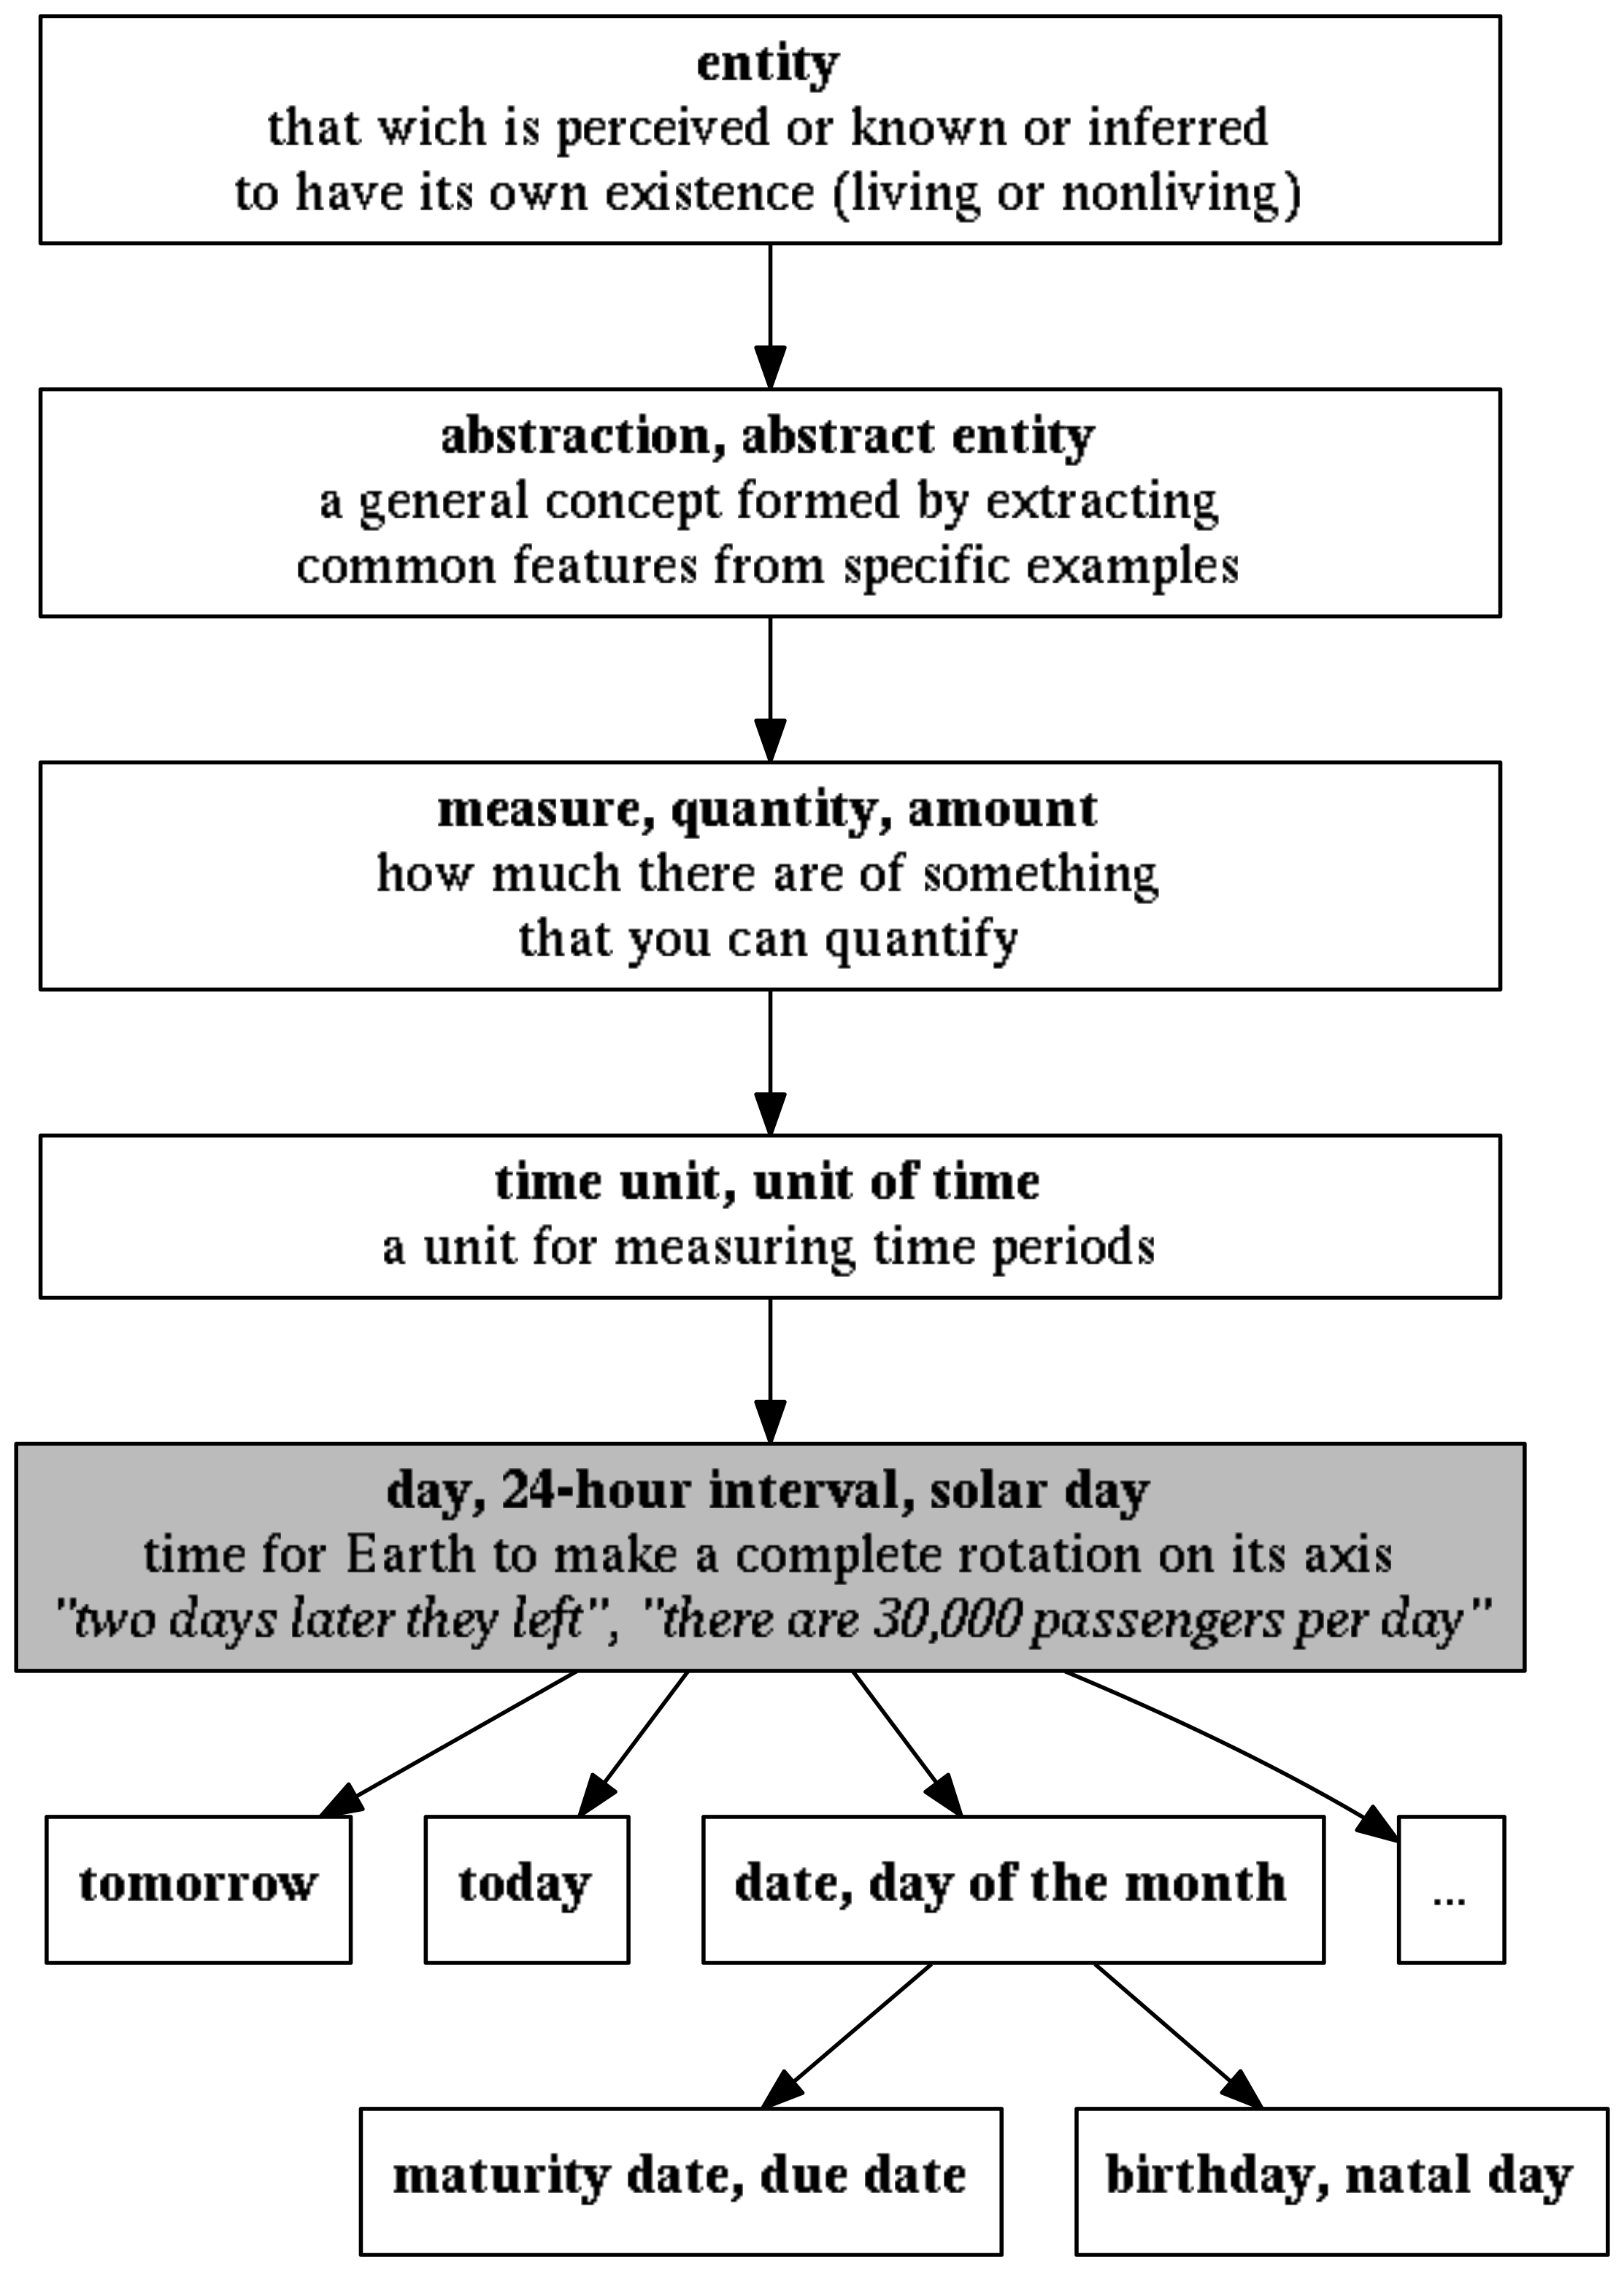
\includegraphics[width=0.6\textwidth]{fig/wordnet_hypernymy.png}
    \caption{\label{fig:wordnet_hypernymy}Hypéronymie dans WordNet autour du
        synset \emph{day}. Les synsets au-dessus de \emph{day} sont ses hypéronymes
        (\emph{day} est-un \emph{time unit}), et les synsets au-dessus font partie de
        ses hyponymes (\emph{tomorrow} est-un \emph{day}).}
\end{figure}

Chaque synset est lié à d'autres synsets à travers un certain nombre de
relations telles que l'hypéronymie, la méronymie de partie (\emph{guidon} est
un méronyme de partie de \emph{vélo}), l'antonymie, etc. Si on ne considère que
l'hypéronymie, WordNet peut être visualisé comme un arbre
(Figure~\ref{fig:wordnet_hypernymy}). En considérant les autres relations,
WordNet est un graphe (Figure~\ref{fig:wordnet_relations}).

\begin{figure}[t]
    \centering
    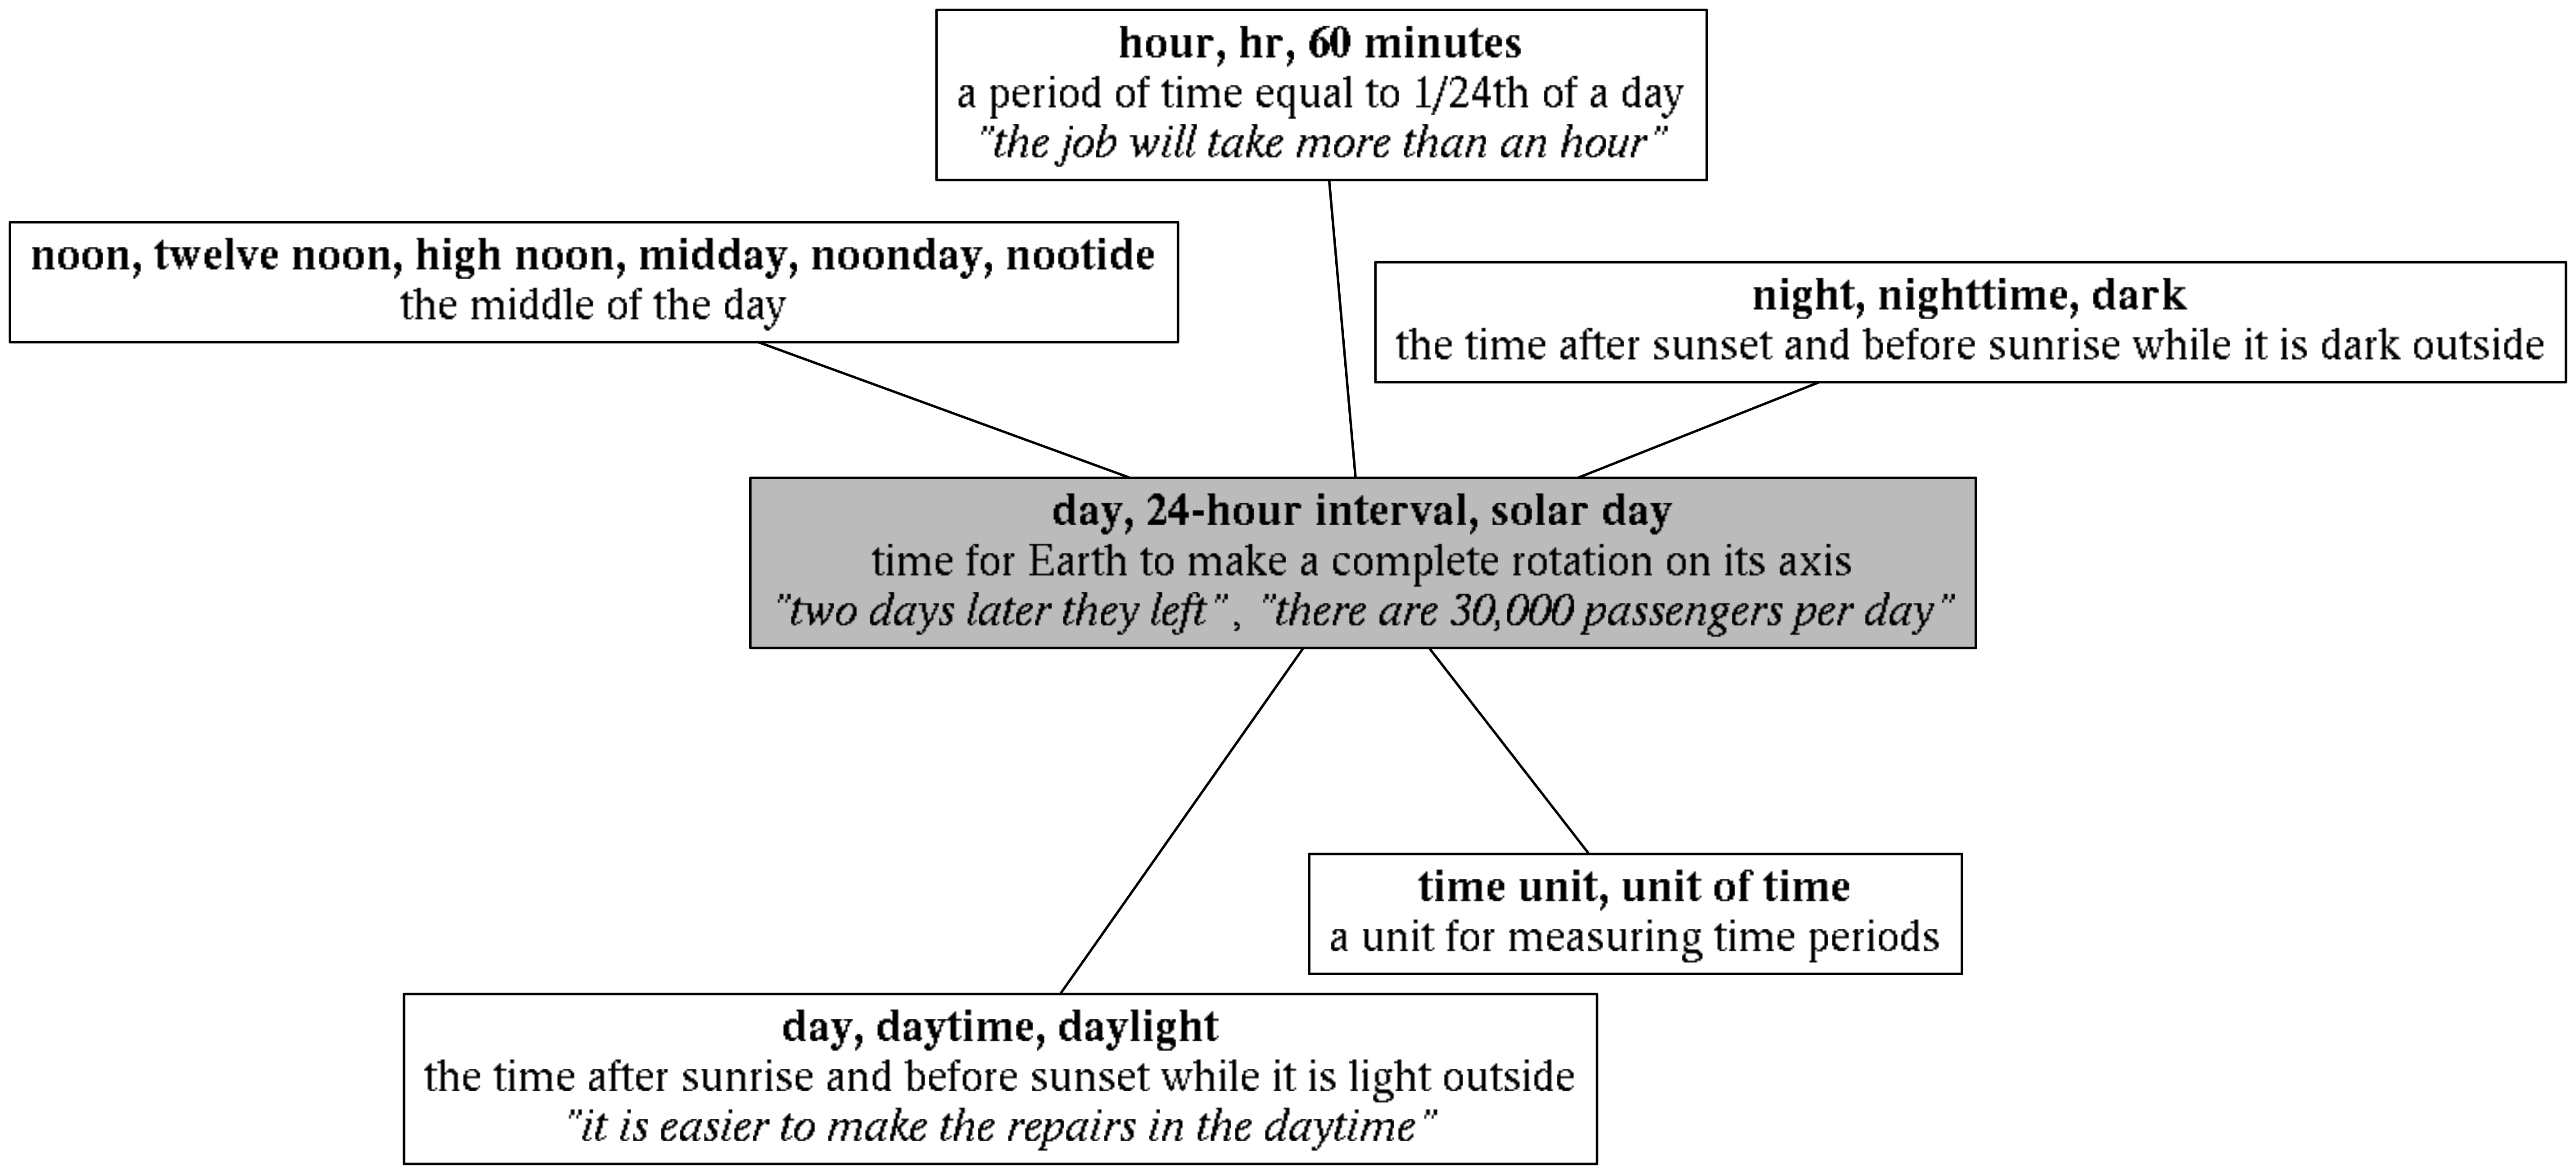
\includegraphics[width=0.7\textwidth]{fig/wordnet_relations.png}
    \caption{\label{fig:wordnet_relations} Le synset \emph{day} est aussi lié à
        d'autres synsets si on considère d'autres relations que l'hypéronymie et
        l'hyponymie.}
\end{figure}

% TODO cite bond survey
Les sens proposés ont étés utilisés pour annoter différents corpus dont le
corpus SemCor, ce qui a permis d'entraîner des systèmes supervisés. WordNet est
rapidement devenu le standard de la désambiguïsation lexicale et a été utilisé
dans de nombreuses campagnes d'évaluation \citep{navigli2009word}. C'est aussi
une ressource très utilisée de manière générale dans le domaine du Traitement
Automatique des Langues\footnote{Au moment de l'écriture de ce manuscrit, ses
10~000 citations sur Google Scholar sont le meilleur moyen de l'attester.}.

\subsection{Les classes de Levin}

\cite{levin1993english} est une classification des verbes anglais établie
suivant un principe simple : le comportement syntaxique des verbes détermine en
partie leur sens. Après avoir défini un certain nombre d'alternances de
diathèses possibles, les verbes sont classés en groupes partageant les mêmes
alternances.

% TODO exemple d'alternance venant vraiment de Levin.

Cette classification a trois intérêts pour l'annotation en rôles sémantiques :

\begin{itemize}

    \item Une grande majorité des verbes anglais sont couverts, rendant la
        ressource utile pour des annotations à large échelle.

    \item La classification est hiérarchique et regroupe de nombreux verbes :
        avec une cinquantaine de classes principales, des généralisations et
        partages d'informations entre les verbes de classes identiques ou
        proches sont possibles.

    \item Les comportements syntaxiques déterminent les comportements
        sémantiques, ce qui correspond au schéma classique de l'annotation en
        rôles sémantiques qui s'appuie sur une analyse syntaxique.

\end{itemize}

%\subsection{Intersection des classes de Levin}

% TODO raccourcir sans dire de bêtises

Dans les classes de Levin, toute distinction de classe doit s'appuyer sur un
critère clairement observable, tel que le comportement syntaxique ou les
propriétés morphologiques d'un verbe. Et ceci même si la distinction entre deux
classes est motivée par la volonté de prendre en compte une différence
sémantique entre deux groupes de verbes.

Pour cette raison, les groupements de verbes sont parfois grossiers d'un point
de vue sémantique. Ainsi, dans les \textit{put verbs} se trouve la classe
\textit{Pocket} qui regroupe les verbes "mettre dans sa poche" (\emph{put}) et
"mettre en prison" (\emph{jail}). Cependant, le comportement syntaxique est le
même : le regroupement est logique et les différences de sens ne sont a priori
pas gênantes pour des tâches telles que l'annotation en rôles sémantiques qui
ne se basent pas sur le sens précis des verbes. Il est possible d'affiner
automatiquement les classes de Levin en réalisant des intersections de classes
: les verbes obtenus seront alors définis plus strictement
\citep{dang1998investigating}. Cette possibilité n'est cependant pas utilisée
dans nos travaux.

\subsection{VerbNet}
\label{subsec:presentation_verbnet}

VerbNet \citep{kipperschuler2005verbnet} est une version électronique des
classes de Levin qui ont été améliorées sur plusieurs fronts avec :

\begin{itemize}

    \item de nouvelles classes provenant de \cite{korhonen2004extended}
        intégrant les verbes acceptant des complétives, mais aussi des
        syntagmes adjectivaux et adverbiaux ou encore des particules,

    \item de nouveaux verbes provenant de \cite{dorr2001lcs},

    \item la liaisons des verbes à WordNet, OntoNotes, PropBank et FrameNet
        dans le cadre du projet SemLink \citep{palmer2009semlink}

    \item de nombreuses corrections au fil des versions, une des améliorations
        prévues dans le futur étant d'ajouter d'autres verbes via l'étude de
        large corpus \citep{bonial2013expanding}.

\end{itemize}

Ces améliorations ont à la fois contribué à VerbNet en largeur (nouvelles
classes) et en profondeur (nouveaux verbes, nouvelles constructions
syntaxiques). La base de données continue d'évoluer, la dernière version au
moment de l'écriture de ce manuscrit étant la 3.2. Malheureusement, la version
3.2 évolue sans que soient marqués clairement les sous-versions : suivant le
jour de téléchargement de VerbNet, nous pouvons avoir à disposition la version
3.2.1, 3.2.2 ou 3.2.3, sans pouvoir clairement distinguer ces trois versions.
Pour cette raison, nous rendons disponibles la version 3.2 de VerbNet que nous
utilisons dans l'ensemble de ce travail à l'adresse suivante : \url{TODO}.

% TODO mieux décrire la hiérarchie et ses niveaux
VerbNet contient 3769 lemmes, 5257 entrées réparties en 500 sous-classes dont
270 classes de niveau 2 et 109 classes de niveau 1. La hiérarchie est
relativement plate. Pour chaque (sous-)classe, ce lexique indique :

\begin{itemize}
        \item la liste des verbes de la classe,
        \item les rôles thématiques en jeu ainsi que leur restrictions de sélection,
        \item la liste des \emph{frames} VerbNet.
\end{itemize}

Une frame inclut une phrase d'exemple, une formule syntaxique donnant la
liaison entre les syntagmes et les rôles thématiques, une formule sémantique
basée sur la logique des prédicats explicitant la relation entre les
participants et les évènements.

% TODO exemple

% TODO autre exemple non intuitif avec verbe complet en bas

% TODO Introduire fig:example_srl
 VerbNet a montré la cohérence de sa classification et est très
utilisé, notamment pour l'annotation en rôles sémantiques
\citep{swier2005exploiting,palmer2013semantic} où il présente l'intérêt de ne
pas être restreint à un domaine spécifique tout en couvrant une large partie
des occurrences des verbes anglais dans un texte donné.

\begin{figure}[ht]
    \centering
    \begin{tabular}{ccc}
        \toprule
        Carol & crushed   & the ice \\
        Agent & V         & Patient \\
        \midrule
        The ice & crushes & easily  \\
        Patient & V       &         \\
        \bottomrule
    \end{tabular}

    \caption{\label{fig:example_srl}Ces deux phrases annotées avec la classe
    VerbNet carve-21.2 mettent en évidence que la position des arguments ne
détermine pas directement les rôles: le sens et la voix de \textit{crush} ne
change pas mais l'annotation sémantique est différente.}

\end{figure}


\subsection{Les Verbes Français et Lexique-Grammaire}

% TODO mieux structurer : avantage *puis* inconvénient (ou l'inverse)
À partir des années 70 deux ressources lexicales pour les verbes français ont
été dévelopées : LVF et LG\footnote{Plus tard, dans les années 1990, une autre
ressource a été dévelopée : Dicovalence. Nous ne l'utilisons presque pas dans
nos travaux.}. Pourquoi ne pas utiliser ces ressources directement ? Un des
intérêts des classes de Levin et de VerbNet par rapport aux ressources
françaises est leur approche pragmatique qui se traduit notamment par l'absence
de prise en compte des emplois métaphorique d'un verbe donné. Ainsi, les tables
du LADL incluent des usages tels que \textit{L'idée gallopait dans son esprit}
qui peuvent induire en erreur une application. Certains usages métaphoriques
peuvent certes être prise en compte dans VerbNet, mais ils n'y sont pas par
défaut. En effet, \cite{brown2012semantic} proposent une analyse systématique
des emplois métaphorique de deux verbes représentatifs et montrent qu'utiliser
VerbNet pour raisonner sur les emplois métaphorique d'un texte est en partie
possible au prix d'une complexité plus importante et de prédicats sémantiques
moins précis.

% TODO mieux que sous-sous-sous et nombre de E2f.1
LVF (Les Verbes Français, \cite{dubois1997verbes}) contient environ 25000
entrées classées en 14 classes sémantiques, 54 sous-classes
syntactico-sémantiques, 248 sous-sous-classes et XXX sous-sous-sous-classes.

% TODO exemple

LG (Lexique-Grammaire, \cite{gross1975methodes,boons1976structure}) comporte
lui 14 000 entrées classifiées en 67 «~tables~», chaque table groupant des
verbes partageant la même propriété définitoire syntaxique et potentiellement
une sémantique similaire. Chaque colonne de la table encode des restrictions
supplémentaires s'appliquant à certains des verbes de la table.

% TODO exemple


Les classes LVF et les tables LG peuvent toutes les deux être comparées aux
classes VerbNet. Cependant, ces ressources n'encodent ni les rôles thématiques
ni les formules sémantiques \footnote{Les notions de rôles thématiques et
d'évènement n'étaient pas répandues dans les années 1970.}.  C'est la raison
principale pour laquelle nous voulons construire une nouvelle ressource
française, \verbenet{} (Chapitre~\ref{ch:verbnet}). Cette ressource tire profit
d'une part des ressources existantes pour le français avec un encodage
sémantique et syntaxique riche, et d'autre part de l'information sémantique
présente dans VerbNet pour l'anglais, une langue proche du français.

\section*{Conclusion}

Après avoir introduit le cadre de nos travaux et présenté les différentes
ressources que nous utilisons, le chapitre suivant présente l'état de l'art qui
est le socle sur lequel nos travaux s'appuient.


% vim: set spelllang=fr:

\setchapterpreamble[ur][.5\textwidth]{%
  \dictum[Robin Hobb, \textit{Assassin's Quest}]{%
As for me, I had been amazed at how many pieces there were to something that had seemed to be all one thing when I had started in on it. [...] All these sounds to make a word, all these words to frame a thought. Language came apart in my hands. I had never stopped to consider it before.}}

\chapter{État de l'art} 
\label{ch:etatdelart} 
% TODO Questions :
%   - inventaires vs. inventaires de sens
%   - qui citer pour sème ?
%   - qui citer pour plus d'un sens ?
%   - réutiliser la figure d'un papier ?


La représentation du sens des mots (section~\ref{sec:mots}) occupe une place
importante dans nos travaux, en particulier pour la traduction de la ressource
WordNet (Chapitre~\ref{ch:wonef}). La traduction de ressources lexicales
(section~\ref{sec:translation}) est un moyen de faire profiter une langue cible
d'une ressource existante dans une autre langue, comme nous le faisons dans la
partie~\ref{part:translation}. Enfin, l'annotation en rôles sémantiques
(section~\ref{sec:srl}) sera elle surtout utile pour la partie~\ref{part:srl}.

\section{Représentation des mots}
\label{sec:mots}

% TODO \citep{harnad1990symbol} ?
Nous étudions ici différentes façons de représenter les mots et leur sens en
commençant par les dictionnaires, puis en étudiant différentes ressources
lexicales représentant le sens des mots. Enfin, nous présentons les modèles de
langue qui sont une manière plus directe de représenter les mots à partir d'un
corpus.

\subsection{Représentation du sens des mots}
\label{subsec:sens_mots}

La lexicographie est la science qui consiste à recenser les mots, les classer,
les définir et les illustrer, par des exemples ou des expressions, pour rendre
compte de l'ensemble de leurs significations et de leurs acceptions au sein
d'une langue, afin de constituer un dictionnaire
\citep{wikipedia2014lexicographie}. La lexicographie est donc un socle sur
lequel le Traitement Automatique des Langues peut s'appuyer pour représenter le
sens des mots.

Pour pouvoir identifier les différents sens d'un mot, les lexicographes
n'opèrent pas par intuition linguistique \citep{kilgarriff1997don}. Ils
commencent par établir un corpus équilibré et de taille assez importante pour
représenter la langue étudiée. Ce corpus peut par exemple être constitué de
textes de journaux, de fiction, ou encore de blogs, le tout étant supposé être
représentatif de ce qu'une personne lambda lit durant sa vie. Pour un mot
donné, le lexicographe examine ses différents usages dans ce corpus dans le but
de séparer ces différents usages en sens. Certains sens, jugés trop peu
fréquents, sont laissés de côté. Une fois la séparation effectuée, le
lexicographe l'étudie pour établir des critères objectifs distinguer les
différents sens du mot étudié. Une phase d'ajustement de la séparation suit
pour vérifier que les critères ont été correctement appliqués, ce qui peut
amener à raffiner ces critères. Une fois le processus fini, ces critères
serviront pour écrire la définition, et les occurrences de mots dans le corpus
pourront servir d'exemples. L'avantage principal est que le processus
lexicographique est désormais basé sur des données réelles et non pas sur des
intuitions linguistiques.

% exemple

Ainsi, les sens ne sont pas définis en tant que tels, mais sont avant tout des
occurrences dans un contexte donné. C'est une façon de comprendre la citation
de \citep{firth1957synopsys} : \emph{You shall know a word by the company it
keeps}\footnote{Vous devriez connaître un mot par ce qui l'accompagne.}. En
effet, selon \citep{kilgarriff1997don}, un ensemble de sens n'est défini que
par rapport à un corpus, et il est illusoire de vouloir définir un dictionnaire
parfait pour tous les sens possibles d'un mot.  Néanmoins, il n'est pas
concevable de réaliser manuellement un dictionnaire par corpus ; et il faut
simplement être conscient des difficultés théoriques posées par le sens des
mots.

Sans s'attarder sur des difficultés théoriques, on considèrera dans ce travail
que les sens définis dans un dictionnaire classique relèvent du «~domaine
général~», et que les sens qui apparaissent dans d'autres domaines sont des
sens «~spécialisés~». Par exemple, le dictionnaire DicoInfo \citep{corpusolst}
spécialisé dans les domaines de l'Informatique et d'Internet mentionne un sens
spécifique pour le nom \emph{compilation} : \emph{action effectuée par un
compilateur qui consiste à transformer du code créé au moyen d'un langage de
programmation évolué en un langage compréhensible par l'ordinateur}. Ce sens
est par exemple absent du TLFi \citep{TLFi} parce qu'il ne faisait pas partie
des sens du mot dans le corpus utilisé pour établir les définitions.

\subsection{Ressources lexicales : WordNet et autres inventaires de sens}
\label{subsec:ressources_lexicales}

D'autres moyen existent pour représenter le sens des mots. La qualité du
travail lexicographique exposé dans les dictionnaires n'a pas été remise en
cause, mais :

\begin{itemize}

    \item les dictionnaires traditionnels, même dans leur version en ligne, ne
        tirent pas profit des nouveaux moyen d'organisation rendus possibles
        avec un ordinateur : il n'est plus nécessaire de trier les mots, on
        peut les représenter par un graphe
        \citep{miller1990introduction,polguere2013tissage},

    \item les dictionnaires traditionnels sont basés sur l'histoire des mots au
        lieu de considérer les progrès en linguistique et psycholinguistique
        proposant des organisations plus utiles et plus proches du lexique
        mental \citep{miller1990introduction}.

\end{itemize}

De plus, l'utilisation de dictionnaires récents implique un coût d'achat et le
respect de la licence restrictive, ce qui explique que ces dictionnaires ont
rapidement étés abandonnés en TAL au profit d'autres ressources disponibles
sous une licence libre comme WordNet, Wikipédia ou encore le Wiktionnaire. En
effet, ces ressources autorisent une utilisation à la fois à des fins de
recherche mais aussi pour un usage commercial, ce qui leur a assuré une large
diffusion.

La première ressource lexicale à tirer partie de la possibilité de représenter
le lexique sous la forme d'un graphe est WordNet, dont l'élaboration a commencé
en 1985 \citep{miller1990introduction}. Établi sur des principes
psycholinguistiques, WordNet propose quatre graphes pour les quatre parties du
discours formant une classe ouverte : noms, verbes, adjectifs, adverbes. Les
nœuds du graphe sont des ensembles de synonymes (\emph{synonym sets} ou
\emph{synsets}). Un synset regroupe plusieurs mots, une définition, et
potentiellement des exemples.

% TODO placement des figures une fois le texte un peu plus stable

\begin{figure}[t]
    \centering
    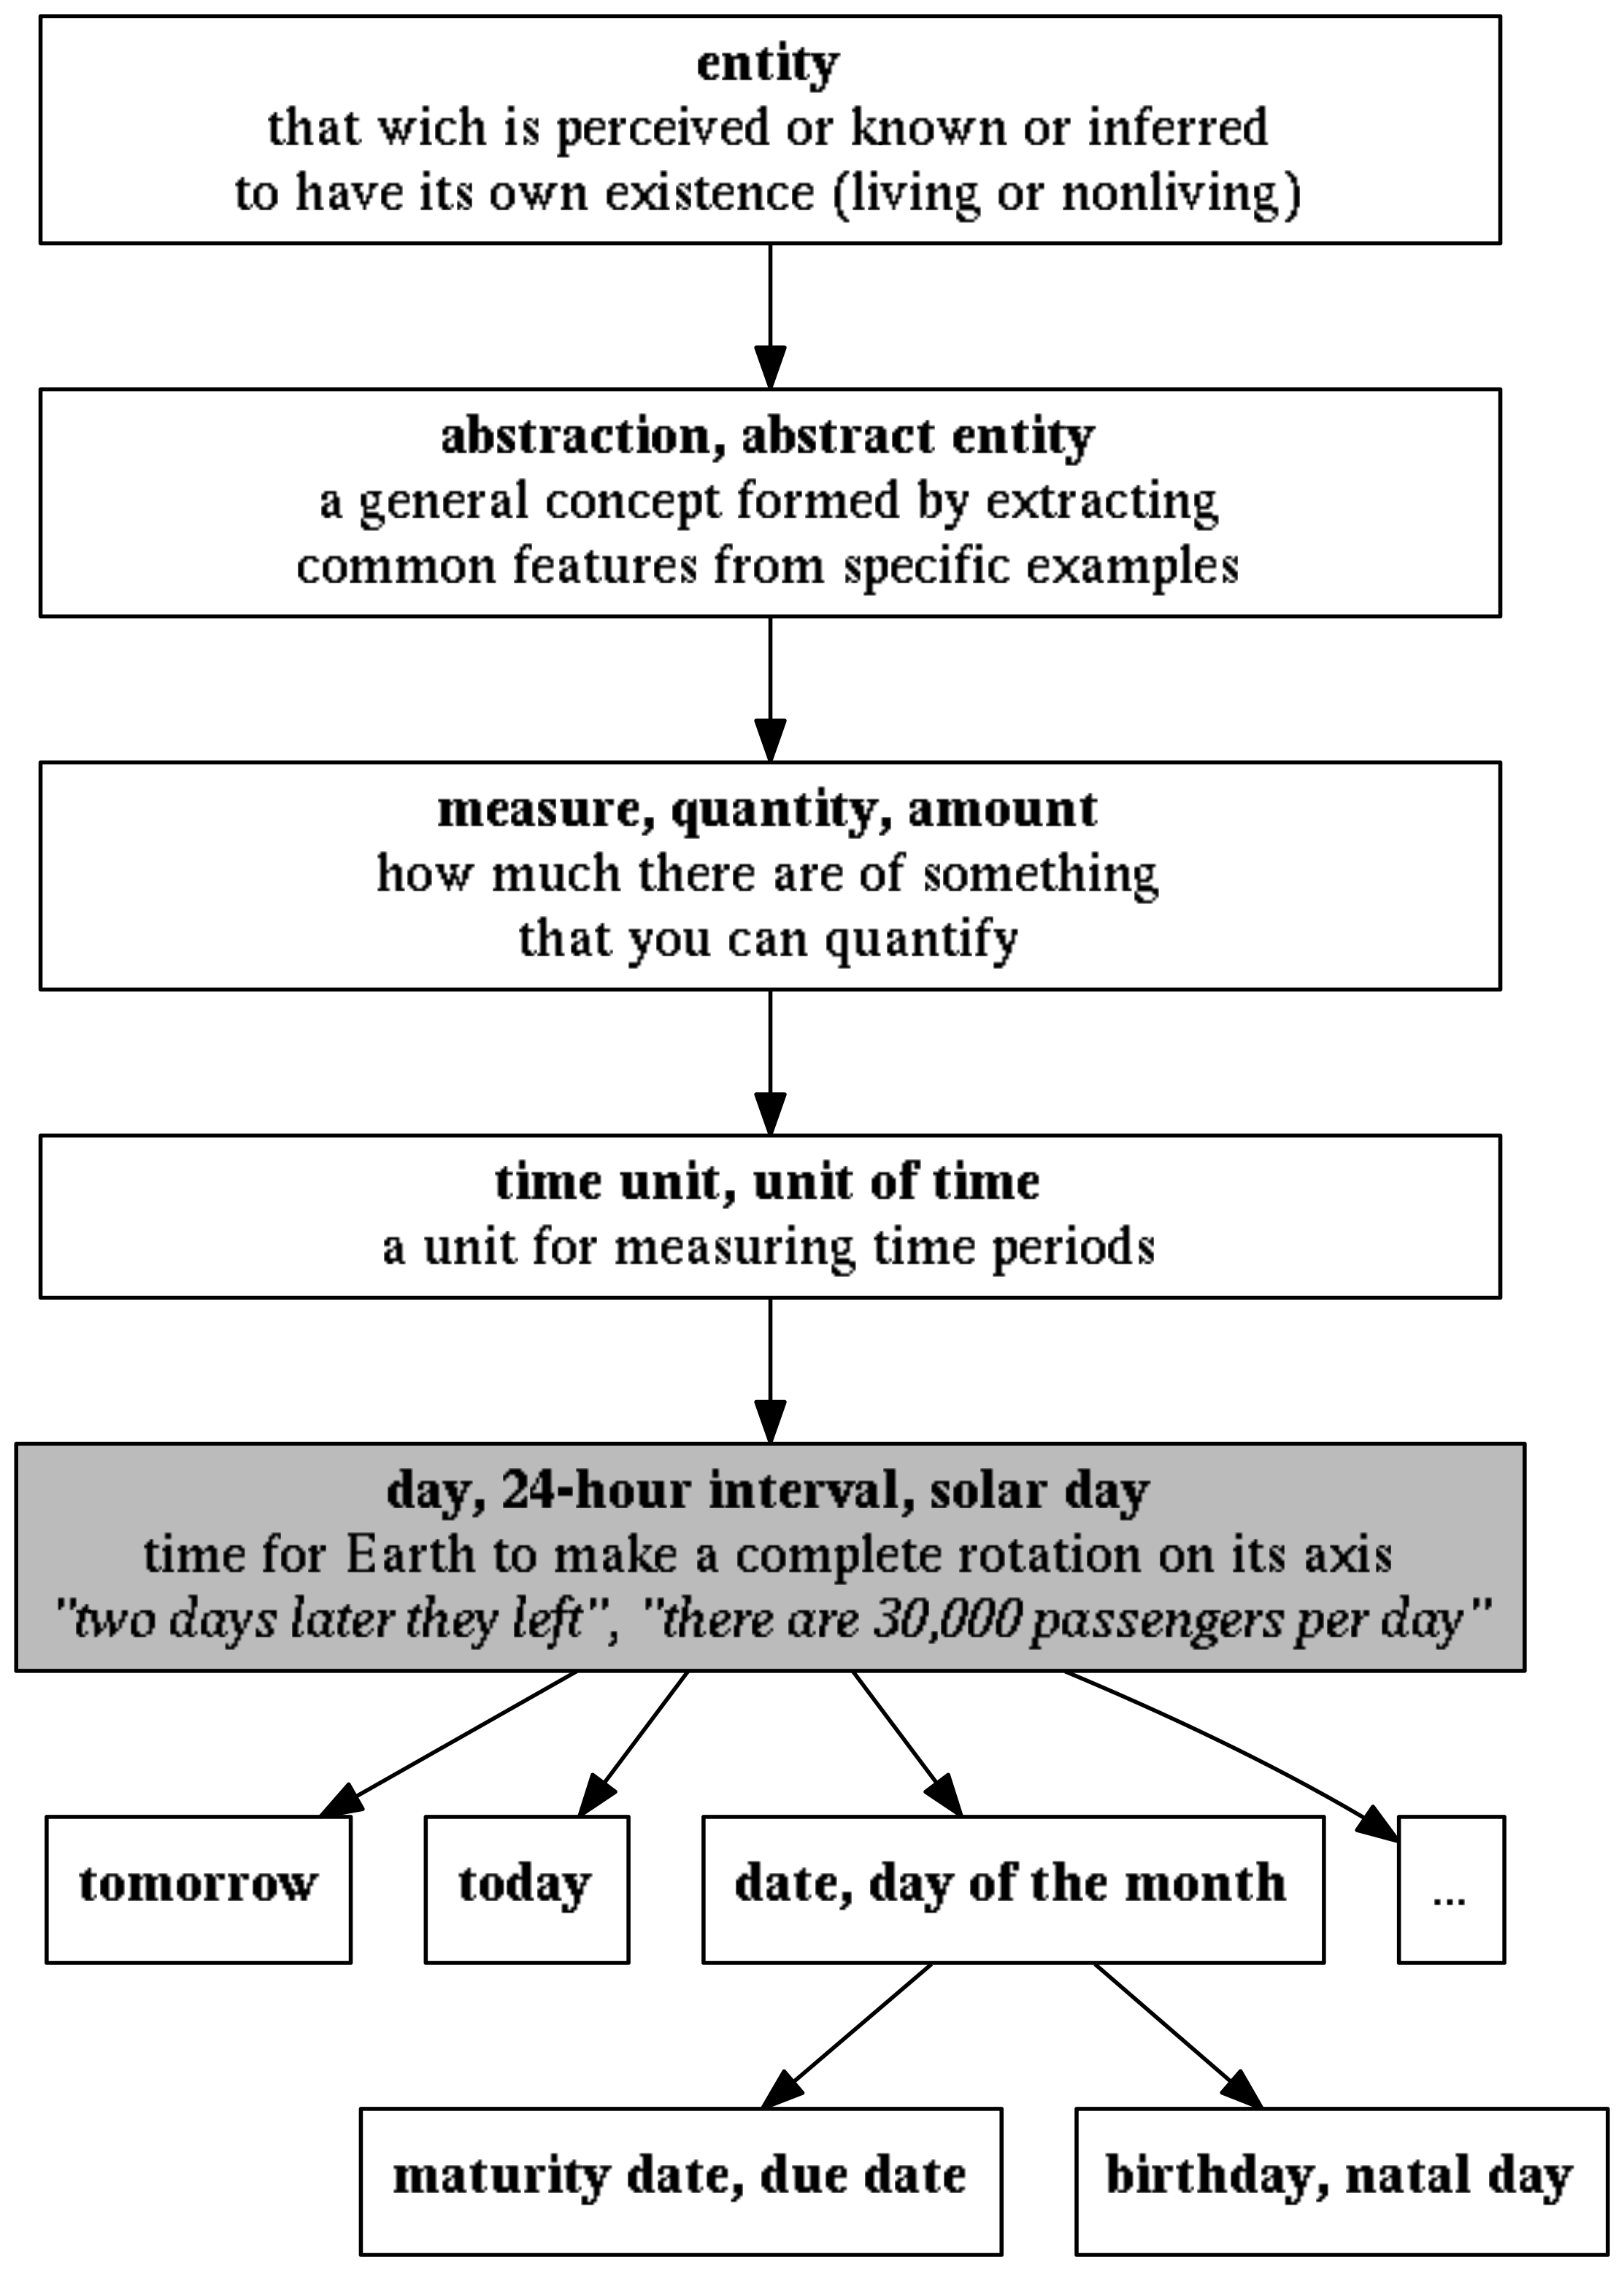
\includegraphics[width=0.6\textwidth]{fig/wordnet_hypernymy.png}
    \caption{\label{fig:wordnet_hypernymy}Hypéronymie dans WordNet autour du
        synset \emph{day}. Les synsets au-dessus de \emph{day} sont ses hypéronymes
        (\emph{day} est-un \emph{time unit}), et les synets au-dessus font partie de
        ses hyponymes (\emph{tomorrow} est-un \emph{day}).}
\end{figure}

Chaque synset est lié à d'autres synsets à travers un certain nombre de
relations telles que l'hypéronymie, la méronymie de partie (\emph{guidon} est
un méronyme de partie de \emph{vélo}), l'antonymie, etc. Si on ne considère que
l'hypéronymie, WordNet peut être visualisé comme un arbre
(Figure~\ref{fig:wordnet_hypernymy}). En considérant les autres relations,
WordNet est un graphe (Figure~\ref{fig:wordnet_relations}).

\begin{figure}[t]
    \centering
    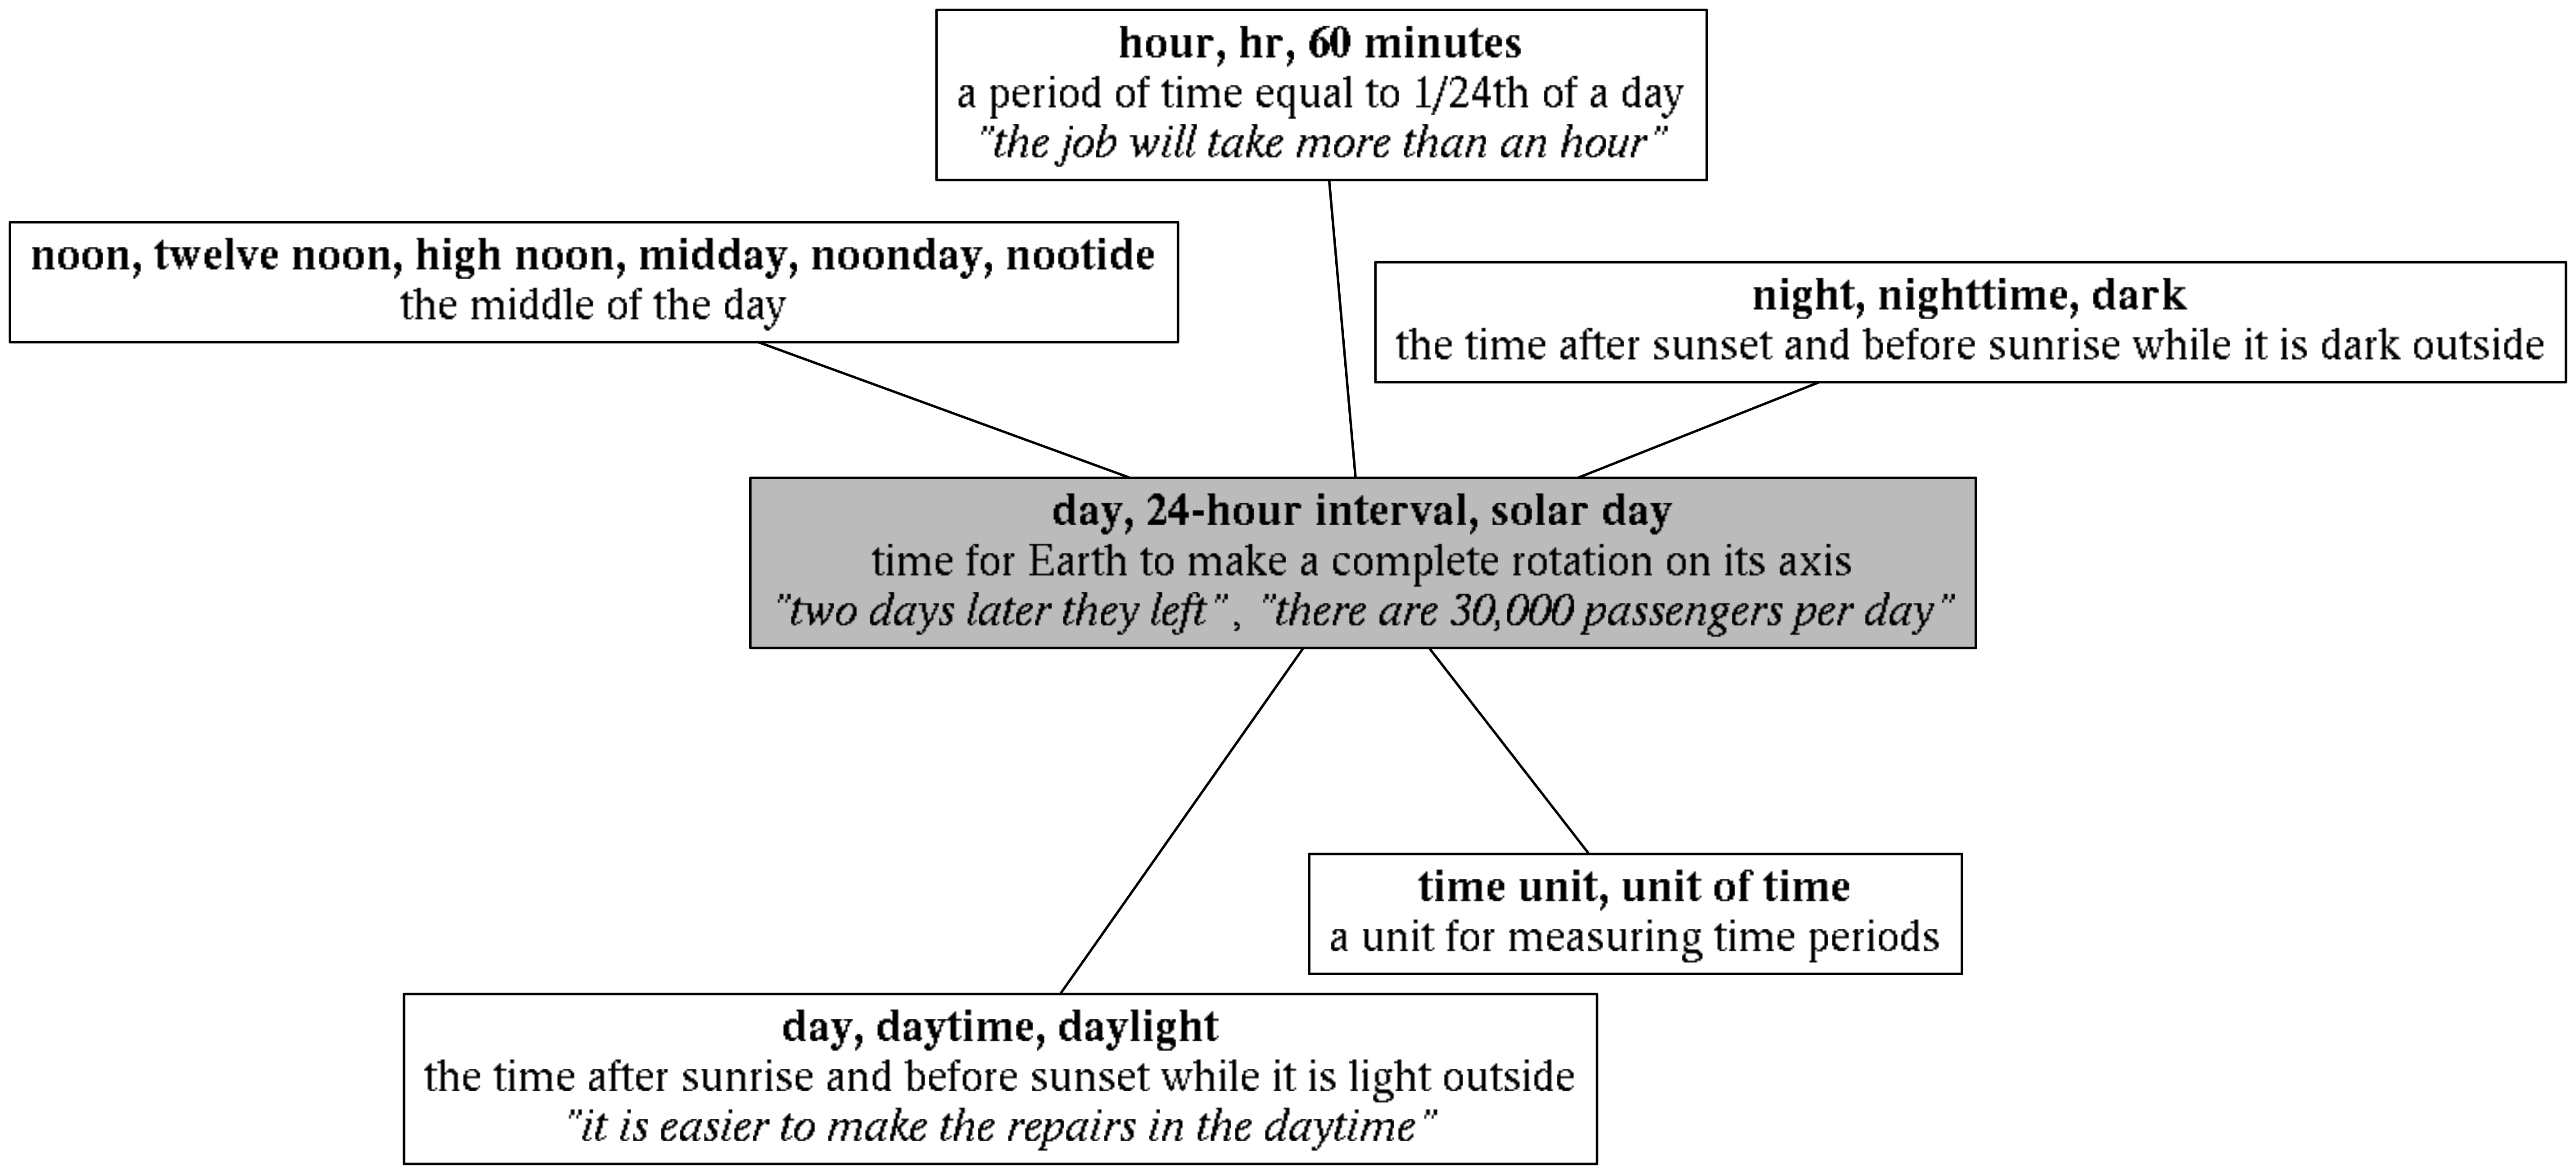
\includegraphics[width=0.7\textwidth]{fig/wordnet_relations.png}
    \caption{\label{fig:wordnet_relations} Le synset \emph{day} est aussi lié à
        d'autres synsets si on considère d'autres relations que l'hypéronymie et
        l'hyponymie.}
\end{figure}

Les sens proposés ont étés utilisés pour annoter différents corpus dont le
corpus SemCor, ce qui a permis d'entraîner des systèmes supervisés. WordNet est
rapidement devenu le standard de la désambiguïsation lexicale et a été utilisé
dans de nombreuses campagnes d'évaluation \citep{navigli2009word}. C'est aussi
une ressource très utilisée de manière générale dans le domaine du Traitement
Automatique des Langues\footnote{Ses 10~000 citations sur Google Scholar au
moment de l'écriture de ce manuscrit sont le meilleur moyen de l'attester}.

Depuis 2006, différents travaux \citep{hovy2006ontonotes,navigli2007semeval}
ont jugé que les défauts attribués à WordNet
\citep{boyd2006adding,ide2006making,snow2007learning} étaient suffisamment
importants pour nécessiter une alternative avec des sens distingués plus
grossièrement. Ce problème est attribué selon \cite{edmonds2002introduction} au
manque de rigueur lexicographique de WordNet, et à la mise en avant de la
similarité entre les mots à travers les synsets au détriment de la distinction
des sens. Il s'est en effet avéré que l'accord inter-annotateurs pour un
étiquetage avec WordNet est faible (de l'ordre de 70\%), et qu'utiliser un
autre inventaire un moyen efficace de s'adapter à différentes applications
\citep{palmer2004different}. La tendance est désormais à l'utilisation
d'inventaires plus grossiers \citep{navigli2007semeval,navigli2012quick}.
% TODO pour parler de tendance, citer plusieurs auteurs et en 2013/2014

Au-delà des approches statistiques \citep{snow2007learning}, de nouveaux
inventaires de sens ont étés développés :

\begin{itemize}

    \item OntoNotes \citep{hovy2006ontonotes} a choisi de regrouper
        manuellement les sens WordNet jusqu'à obtenir un accord
        inter-annotateur de 90\%.

    \item DANTE\footnote{Les entrées pour les mots entre M et R sont
        disponibles sur http://webdante.com/} \citep{mccarthy2010dante} est un
        inventaire entièrement nouveau, conçu dans l'objectif de corriger les
        erreurs faites avec WordNet\citep{kilgarriff2010detailed}.

    \item Le Réseau Lexical du Français\citep{gader2014lexicon} lie des sens de
        mots avec de nombreuses fonctions lexicales associés à un degré de
        confiance, le tout permettant de produire des articles de dictionnaires.

\end{itemize}

Ces inventaires semblent plus adaptés que WordNet pour la désambiguïsation
lexicale \citep{navigli2012quick}, mais ils ne sont pas encore disponibles ou
ne sont pas utilisables librement à des fins commerciales.

Une approche complètement différente est celle de la structure de qualia
\citep{johnston1996qualia} qui s'inscrit dans le contexte plus général du
lexique génératif introduit par \cite{pustejovsky1991generative} qui considère
qu'une approche énumérative n'est pas viable. Le sens d'un mot est alors défini
selon plusieurs aspects prédéfinis (constitution, rôles, facteurs impliqués
dans la création, etc.) qui peuvent se retrouver dans plusieurs mots. Par
exemple, un couteau contient une lame et sert à couper. Cette approche est
semblable à celle qui définit le sens d'un mot comme une simple suite de sèmes.

Enfin, différents travaux mentionnent la possibilité d'utiliser plus d'un sens
pour un mot donné. \cite{smith2011rumble} propose d'utiliser des distributions
de probabilité sur les différents sens possibles pour définir un sens précis
dans un corpus. \cite{erk2013measuring} montrent qu'un accord inter-annotateur
haut peut être obtenu en demandant aux annotateurs d'indiquer pour chaque sens
sa correspondance avec l'usage sur une échelle de 1 à 5. Dans SemCor, les
annotateurs pouvaient choisir plusieurs sens si besoin, mais seulement 0.3\%
des occurrences de SemCor sont étiquetées avec plus d'un sens. Une campagne
d'évaluation a eu lieu en 2013 à ce sujet \citep{jurgens2013semeval}.

\subsection{Modèles de langue pour la similarité sémantique}
\label{subsec:modeles_de_langue}

Un modèle de langue prédit la probabilité d'un mot étant donné son contexte
dans la phrase. C'est directement utile pour des tâches telles que la
traduction automatique ou la reconnaissance de la parole dans lesquelles un
modèle de langue favorisera des phrases plausibles globalement au lieu
d'étudier chaque mot individuellement.

Ce n'est pas l'utilisation que nous faisons des modèles de langues : ici,
l'objectif est d'obtenir des mesures de similarité sémantiques utiles pour
notre traduction de WordNet (Chapitre~\ref{ch:wonef}) et pour notre module de
similarité entre syntagmes pour l'annotation en rôles sémantiques
(Chapitre~\ref{ch:semantic}).

Quelle est l'intuition derrière l'utilisation des modèles de langue ?
L'hypothèse distributionnelle s'explique ainsi
\cite[p.~786]{harris1954distributional} :

\begin{quote} ... si l'on considère que le sens de deux mots ou morphèmes A et B
    diffère davantage que le sens de A et C, alors on observe souvent que les
    distributions de A et B diffèrent davantage que les distributions de A et C.
    Autrement dit, la différence de sens est corrélée à la différence de
    distribution. \end{quote}

Les modèles de langue sont un moyen d'étudier ces distributions de probabilité.
On peut étudier deux types de distributions différentes correspondant à deux
types de relations entre les mots \citep{sahlgren2008distributional} :

\begin{itemize}
    \item les relations syntagmatiques identifient les mots qui sont présents
        ensemble dans un contexte donné ;
    \item les relations paradigmatiques identifient les mots qui sont présents
        dans un même contexte, mais sans y être présents ensemble.
\end{itemize}

Par exemple, étant donné les deux phrases \emph{Je bois du café} et \emph{Je
bois du thé}, on peut déduire que les lemmes \emph{boire} et \emph{thé} sont
liés par une relation syntagmatique : ils sont présents ensemble dans la
phrase. Au contraire, \emph{thé} et \emph{café} ne sont pas ici présents dans
la même phrase, mais apparaissent dans un même contexte (\emph{Je bois du}) :
ils sont liés par une relation paradigmatique.

Observer les distributions de contexte entre les mots permet à la fois
d'évaluer la similarité entre deux mots mais est aussi l'occasion de séparer
les mots suivant leurs sens \citep{yarowsky1993one,pantel2002discovering}. Un modèle de langue brut ne décrit que des lexèmes Nous
serons par la suite essentiellement concernés par les lexèmes : c'est-à-dire la
similarité entre les paires (lemme, sens) mais un modèle de langue ne peut
directement manipuler que des mots : la séparation se fait par la suite.

% \cite{schutze1998automatic,pantel2002discovering,niu2007three,pedersen2010duluth,liu2012semantic} ?

La question qui se pose maintenant que nous voulons observer les distributions
est : comment représenter et calculer ces distributions ? Une façon d'opérer
est de calculer la probabilité d'un mot dans une phrase étant donné les mots
précédents. Par exemple, étant donné le début de phrase "Au-delà des approches
...", on veut connaître la probabilité du mot suivant, en espérant que celle de
\emph{statistiques} ou \emph{supervisées} soit plus importante que celle de
\emph{chat}. En prenant par exemple le contexte des deux mots qui précèdent le
mot étudié, on calcule sa probabilité simplement avec le maximum de
vraisemblance :

\[
p(w_i|w_{i-2}, w_{i-1}) = \frac{compte(w_{i-2}, w_{i-1}, w_i)}{compte(w_{i-1}, w_i)}
\]

La séquence $w_{i-2}, w_{i-1}, w_{i}$ est un 3-gramme, et $compte$ compte le
nombre d'occurrences de cette séquence dans le corpus considéré. La taille du
contexte peut varier, ce qui est la raison pour laquelle on parle de manière
générale de n-grammes. Le nombre de paramètres à estimer pour obtenir une
distribution de probabilité conditionnelle fiable dépend de la taille du
vocabulaire ($|V|$) et de la taille du contexte étudié ($n$) et vaut $|V|^n$.
En considérant un petit vocabulaire (10~000 mots) et un contexte de trois mots,
il faut déjà estimer $10^{12}$ probabilités, ce qui requiert un corpus très
large : Google a utilisé un corpus de livres d'un trillion de mots pour estimer
ses n-grammes allant jusqu'à $n=5$ \citep{brants2006web}. Diverses techniques
de lissage existent pour mieux répartir les probabilités
\citep[Chapitre~4]{jurafsky2008speech}. En effet, la plupart des probabilités
sont initialement nulles, que ce soit parce que le n-gramme est
grammaticalement invalide ou simplement parce qu'il n'a pas été observé dans le
corpus étudié. Il faut leur assigner une probabilité très faible afin d'éviter
de multiplier des probabilités nulles et de perdre ainsi de l'information.

Diverses extensions de ces modèles de langues à base de n-grammes existent,
l'une d'entre elles étant le modèle de langue syntaxique
\citep{lin1998automatic,goldberg2013dataset}. Dans ce modèle, on considère les
mots présents ensemble dans une relation syntaxique donnée. Pour la relation
complément du nom par exemple, on s'attend à ce que \emph{vélo} soit le
complément du nom des mots \emph{pédale}, \emph{guidon}, \emph{pneu} et ainsi
de suite. Le modèle de langue syntaxique que nous utilisons pour traduire
WordNet a été entraîné sur un corpus extrait du web francophone
\citep{grefenstette2007conquering}. Le corpus a ensuite été analysé par LIMA
\citep{besancon2010lima}, une chaîne d'analyse linguistique désormais libre ici
utilisée comme un analyseur syntaxique à base de règles produisant des
dépendances syntaxiques fines. Pour une relation donnée $r$ et un lemme $x$, le
modèle de langue indique quels sont les 100 premiers lemmes co-occurrant le
plus fréquemment avec $x$ dans la relation $r$.  Avec le mot \textit{avion} et
la relation de complément du nom, le mot \textit{billet} modifie le plus
\textit{avion} : \textit{billet d'avion} est fréquent dans le corpus. Ce modèle
de langue peut-être visualisé sur
\url{http://www.kalisteo.fr/demo/semanticmap/}.

D'autres types de modèles de langue représentent les mots de manières
distribuée en utilisant un vecteur de nombres réels. La manière la plus
répandue pour faire cela est d'utiliser un réseau de neurones dont une des
couches sera le vecteur représentant chaque mot. \cite{hinton1986learning} a
d'abord proposé l'idée d'un réseau de neurones pour représenter des concepts,
puis \cite{bengio2001neural,bengio2003neural} ont proposé le modèle de langue
neuronal tel qu'on le connaît aujourd'hui. Ce modèle de langue calcule non
seulement la probabilité d'un mot étant donné les mots précédents : c'est la
tâche sur laquelle il est entraîné. Mais il obtient aussi une représentation de
chaque mot où les mots sémantiquement proches ont des représentations proches.

% TODO LSA fait une partie du chemin
% TODO collobert & weston ? liens entre rns ?

\cite{mikolov2013efficient} et l'outil word2vec
associé\footnote{\url{https://code.google.com/p/word2vec/}} ont rendu possible
l'application de tels réseaux de neurones accessible et efficace. Une propriété
particulièrement intéressante des réseaux de neurones obtenus est que la
distance entre certains mots est fixe. En particulier, dans cet espace de
vecteurs :

\begin{itemize}
    \item reine + homme - femme = roi
    \item Paris - France + Spain = Madrid
    \item Australian - Australia + France = French
\end{itemize}

Ces résultats non prévus (la tâche était uniquement de prédire le mot en
fonction de son contexte) illustrent le type de généralisation obtenues à
l'aide d'un réseau de neurones et qui seraient autrement inaccessibles.

Ces réseaux de neurones sont encore difficiles à entraîner et à paramétrer
\citep{do2014modeles}, mais représentent une alternative bien plus efficace que
les modèles de langue simples à base de n-grammes parce qu'ils généralisent
bien mieux que la simple utilisation du maximum de vraisemblance
\citep{olah2014deep}.

% TODO donner des raisons de l'efficacité, "exponentiel" tout ça

\section{Traductions de ressources linguistiques}
\label{sec:translation}

\subsection{WordNet}

WordNet reste une ressource extrêmement utile et reproduire ce travail pour
d'autres langues serait coûteux et difficile à maintenir. Et malgré quelques
problèmes théoriques, traduire WordNet en gardant sa structure et ses synsets
mène à des ressources linguistiques utiles
\citep{fellbaum2007connecting,demelo2008utility}. Il n'existe encore que peu
d'équivalents de même qualité dans d'autres langues \citep{bond2012survey}.

Les traductions automatiques de WordNet emploient une approche dite d'extension
(\textit{extend approach}) : la structure de WordNet est préservée et seuls les
littéraux sont traduits. Trois techniques principales représentent cette
approche dans la littérature. La plus simple utilise des dictionnaires
bilingues pour faciliter le travail des lexicographes qui filtrent ensuite
manuellement les entrées proposées
\citep{vossen1998eurowordnet,pianta2002developing,tufis2004balkanet}. Une
deuxième méthode de traduction utilise des corpus parallèles, ce qui évite
l'utilisation de dictionnaires qui peuvent entraîner un biais lexicographique.
\cite{dyvik2004translations} représente cette méthode en s'appuyant sur des
\textit{back-translations} entre le norvégien et l'anglais, alors que
\citep{sagot2008construction} combinent un lexique multilingue et les
différents WordNets de BalkaNet comme autant de sources aidant à la
désambiguïsation. Enfin, plus récemment, des ressources telles que Wikipédia ou
le Wiktionnaire ont été explorées. Grâce aux nombreux liens entre les
différentes langues de ces ressources, il est possible de créer de nouveaux
wordnets \citep{demelo2009towards,navigli2010babelnet} ou d'améliorer des
wordnets existants \citep{hanoka2012wordnet}.
% TODO mettre à jour l'état de l'art avec GWC 2014 et LREC 2014 ?

Concernant le français, l'EuroWordNet \citep{vossen1998eurowordnet} est la
première traduction française de WordNet. C'est une ressource d'une couverture
limitée qui demande des améliorations significatives avant de pouvoir être
utilisée \citep{jacquin2006systemes}, et qui n'est ni libre ni librement
accessible. WOLF est une seconde traduction initialement construite à l'aide de
corpus parallèles \citep{sagot2008construction} et étendue depuis avec
différentes techniques \citep{apidianaki2012applying}. WOLF est distribué sous
une licence libre compatible avec la LGPL et c'est aujourd'hui le WordNet
français standard. Enfin, JAWS \citep{mouton2010jaws} est une traduction des
noms de WordNet développée à l'aide de dictionnaires bilingues et d'un modèle
de langue syntaxique.

\label{subsec:jaws_translation_process}

Pour notre traduction de WordNet nommée WoNeF (Chapitre~\ref{ch:wonef}), nous
reprenons les travaux de \cite{mouton2010jaws} qui ont abouti à JAWS, que nous
présentons ici. C'est un algorithme faiblement supervisé qui ne demande aucune
donnée annotée manuellement. Pour traduire un wordnet source, JAWS s'appuie sur
un dictionnaire bilingue et un modèle de langue syntaxique pour le langage
cible.

Le dictionnaire bilingue est une concaténation du dictionnaire bilingue
SCI-FRAN-EurADic\footnote{\url{http://catalog.elra.info/product_info.php?products_id=666}}
et des liens entre les Wiktionnaires français et
anglais\footnote{\url{http://www.wiktionary.org/}}. Le modèle de langue
syntaxique a été présenté à la section~\ref{subsec:modeles_de_langue}. Grâce
aux dictionnaires, JAWS n'a pas besoin de sélectionner les littéraux de chaque
synset parmi l'ensemble du vocabulaire mais seulement parmi un petit nombre de
candidats (9 en moyenne).  Le processus de traduction se fait en trois étapes :
\begin{enumerate} \item Créer un wordnet vide : la structure de WordNet est
préservée, mais les synsets eux-mêmes n'ont pas de littéraux associés.  \item
Choisir les traductions les plus faciles parmi les candidats des dictionnaires
pour commencer à remplir JAWS.  \item Étendre JAWS de manière incrémentale en
utilisant le modèle de langue, les relations entre synsets et le JAWS déjà
existant.  \end{enumerate}

\paragraph{Sélecteurs initiaux} Quatre algorithmes que nous nommons sélecteurs
initiaux choisissent des traductions correctes parmi celles qui sont proposées
par les dictionnaires. Premièrement, les mots qui apparaissent dans un seul
synset ne sont pas ambigus et il suffit d'ajouter toutes leurs traductions au
WordNet français : c'est le sélecteur par monosémie. C'est le cas de
\textit{grumpy} : toutes ses traductions sont validées dans le synset où il
apparaît. Deuxièmement, le sélecteur par unicité identifie les mots n'ayant
qu'une seule traduction et la valident dans tous les synsets où elle est
présente. Les cinq synsets contenant \textit{pill} en anglais sont ainsi
complétés avec \textit{pilule}. Un troisième sélecteur vise à traduire les mots
qui ne sont pas dans le dictionnaire en utilisant directement la traduction
anglaise : c'est le sélecteur des transfuges. Un quatrième sélecteur utilise la
distance d'édition de Levenshtein : si la distance entre un mot anglais et sa
traduction est petite, on peut considérer que c'est le même sens (c'est le cas
par exemple pour \textit{portion} ou encore \textit{university}), malgré
l'existence de certains faux amis. Ces quatre sélecteurs produisent une
première version du WordNet français qui contient assez de traductions pour
pouvoir ensuite utiliser le modèle de langue et continuer de compléter les
synsets.

\paragraph{Expansion de JAWS} JAWS étant partiellement rempli, une nouvelle étape d'expansion tire parti des relations entre les synsets de WordNet pour valider de nouvelles traductions. Par exemple, si :

\begin{itemize}
    \item un synset S1 est méronyme d'un synset S2 dans WordNet,
    \item il existe un contexte où un littéral dans S1 est méronyme d'un littéral candidat C dans S2,
\end{itemize}
alors ce littéral est considéré comme correct. La tâche de traduction est ainsi réduite à une tâche de comparaison entre d'une part les relations lexicales entre les synsets de WordNet et d'autre part les relations lexicales entre les lexèmes du français.

Prenons l'exemple de \textit{quill} qui peut se traduire par \textit{piquant} ou \textit{plume} (Figure \ref{meronymyexample}). Dans WordNet, \textit{quill} est méronyme de \textit{porcupine} qui a déjà été traduit par \textit{porc-épic} par un sélecteur initial. Dans le modèle de langue, \textit{piquant} fait partie des compléments du noms de \textit{porc-épic} mais ce n'est pas le cas de \textit{plume}. Ici, la relation de complément du nom implique la méronymie et c'est donc \textit{piquant} qu'il faut choisir comme la traduction correcte de \textit{quill}. Le modèle de langue a permis la désambiguïsation parmi les deux traductions possibles.

\tikzstyle{block}=[draw, fill=blue!5, rectangle, minimum height=0.5cm, minimum width=3cm, text width=5cm]

\begin{figure}[ht]
  \centering
  \begin{tikzpicture}[auto, node distance=2cm,>=latex']
    % Inspired from http://www.texample.net/tikz/examples/control-system-principles/
    % first place and connect the outer blocks that represent synsets
      \node [block, text width=5cm] (quill) {~\\\textbf{Synset S1} \\ - Anglais : quill \\ - Français : piquant? plume? \\ (a stiff hollow protective spine on a porcupine) \\ ~ };
      \node [block, text width=4.0cm, right of=quill, node distance=9cm] (porcupine) {\textbf{Synset S2} \\ - Anglais : porcupine, hedgehog \\ - Français : porc-épic \\ (rodents with sharp erectile bristles mingled with the fur)};
    \draw [<-] (porcupine) -- node[above] {méronyme de} (quill);
    \draw [<-] (porcupine) -- node[below] {(relation WordNet)} (quill);

    % then the syntactic model relations
    \node [block, below of=porcupine, text width=4.0cm, node distance=3cm] (porcupinesynt1) {porc-épic};
    \node [block, below of=quill, node distance=3cm] (quillsynt1) {\Large{mémoire}, \Large{piquant}, \large{poil}, \large{épine}, yéti, ragoût, grotte, \small{tactique}, \small{pelage}, \small{dextre}, \small{aiguille}, ...};
    \draw [<-] (porcupinesynt1) -- node[above] {complément du nom de} (quillsynt1);
    \draw [<-] (porcupinesynt1) -- node[below] {(modèle de langue)} (quillsynt1);

  \end{tikzpicture}
  \caption{\protect\centering\label{meronymyexample}Traduction via la relation de méronymie de partie.}
\end{figure}

Un problème potentiel avec cette approche est que la relation de complément du nom n'est pas limitée à la méronymie. Par exemple, le mot \textit{mémoire} qui apparaît dans le modèle de langue vient d'un livre intitulé \textit{Mémoires d'un porc-épic}. Heureusement, \textit{mémoire} n'est pas dans les candidats de \textit{quill} et ne peut pas être choisi comme une traduction. Paradoxalement, le modèle de langue ne peut pas choisir entre deux mots très différents, mais est capable de choisir la traduction correcte d'un mot polysémique. Alors que traduire WordNet automatiquement avec un dictionnaire ou un modèle de langue syntaxique est impossible, combiner les deux ressources permet de résoudre le problème.

Chaque sélecteur suit le même principe que le sélecteur par méronymie de partie
et traduit de nouveaux synsets en identifiant les relations entre lexèmes via
le modèle de langue syntaxique. La correspondance entre la relation de
complément du nom et la relation de méronymie est directe, mais ce n'est pas le
cas pour les autres relations : il n'y a par exemple pas de relation syntaxique
qui exprime directement la synonymie entre deux lexèmes. Pour ces relations, il
est nécessaire d'employer soit des motifs lexicaux \citep{hearst1992automatic}
soit des relations syntaxiques de deuxième ordre \citep{lenci2012identifying}.
Ce sont ces dernières, aussi nommées relations paradigmatiques
(section~\ref{subsec:modeles_de_langue}, que JAWS utilise. Pour la synonymie,
si deux mots partagent les mêmes co-occurents dans une relation syntaxique
donnée, alors ils peuvent être synonymes dans ce contexte. Pour les noms, les
relations syntaxiques qui donnent les meilleurs résultats sont les relations de
complément du nom, d'objet du verbe et d'apposition. Concrètement, si deux noms
qui modifient les mêmes noms sont les objets des mêmes verbes ou sont apposés
aux mêmes noms, alors il est probable qu'ils soient synonymes et si l'un des
deux est déjà dans un synset, alors on peut y ajouter le second. Par exemple,
\textit{avant-propos} et \textit{préface} partagent les mêmes compléments du
noms : \textit{livre, édition, ouvrage}. Le sélecteur par synonymie peut
ajouter \textit{avant-propos} une fois que le littéral \textit{préface} est
dans JAWS. \citep{mouton2010jaws,mouton2010phd} décrivent d'autres sélecteurs
exploitant notamment les relations d'hyperonymie et d'hyponymie.

\subsection{VerbNet}
\label{subsec:presentation_verbnet}

\cite{levin1993english} est une classification des verbes anglais suivant un
principe simple : le comportement syntaxique des verbes détermine en partie
leur sens. Après avoir défini un certain nombre de constructions syntaxiques
possibles, les verbes sont classés en groupes partageant les mêmes
constructions. Le projet VerbNet a exporté les classes de Levin dans un format
électronique (XML) et a étendu la ressource avec de nouvelles classes,
constructions syntaxiques et verbes. VerbNet est une ressource lexicale pour
les verbes anglais organisée autour de classes sémantiques et de sous-classes
syntaxiques : une classe sémantique est divisée en sous-classes de verbes qui
partagent tous le même ensemble de cadres de sous-catégorisation
(Figure~\ref{fig:example_srl}, en suivant \cite{levin1993english}.  Dans sa
version actuelle\url{http://verbs.colorado.edu/~mpalmer/projects/verbnet.html},
VerbNet comprend 3769 lemmes, donnant lieu à 5257 entrées réparties en 274
sous-classes. VerbNet a montré la cohérence de sa classification et est très
utilisé, notamment pour l'annotation en rôles sémantiques
\citep{swier2005exploiting,palmer2013semantic} où il présente l'intérêt de ne
pas être restreint à un domaine spécifique tout en couvrant une large partie
des occurrences des verbes anglais dans un texte donné.

\begin{figure}[ht]
    \centering
    \begin{tabular}{ccc}
        \toprule
        Carol & crushed   & the ice \\
        Agent & V         & Patient \\
        \midrule
        The ice & crushes & easily  \\
        Patient & V       &         \\
        \bottomrule
    \end{tabular}
    \caption{\label{fig:example_srl}Ces deux phrases annotées avec la classe VerbNet carve-21.2 mettent en évidence que la position des arguments ne détermine pas directement les rôles: le sens et la voix de \textit{crush} ne change pas mais l'annotation sémantique est différente.}
\end{figure}

La traduction des classes de Levin et plus récemment de VerbNet dans d'autres
langue est une tâche reconnue comme utile dans la littérature. Initialement,
des méthodes automatiques ont mené à des améliorations dans le VerbNet anglais
lui-mmême après validation manuelle : de nouvelles classes ont été incorporées
\citep{korhonen2004extended} et de nouveaux verbes ont été ajouté à partir de
la base de données LCS \citep{dorr2001lcs} ou avec l'outil Sketch Engine
\citep{bonial2013expanding}. La base de données continue aujourd'hui d'évoluer,
la prochaine version prévue étant la 3.2.4.

Dans d'autres langues, \cite{merlo2002multilingual} ont utilisé des similarités
entres langues pour convertir 20 classes de Levin vers l'Italien. Des
acquisitions automatiques ont aussi été menées en japonais
\citep{suzuki2009classifying}, allemand \citep{im2006experiments} et espagnol
\citep{ferrer2004towards}. Les seules traductions directes dont nous avons la
connaissance sont le VerbNet estonien \citep{jentson2014verbnet} et le VerbNet
portuguais brésilien \citep{scarton2012towards} qui utilise des mappings entre
VerbNet et WordNet, et entre WordNet.Br et WordNet.

Pour le français, \cite{saintdizier1996constructing} a d'abord produit une
ressource proche des classes de Levin. À notre connaissance, l'effort sur cette
ressource a arrêté et le résultat n'est pas disponible. Des travaux se sont
ensuite concentrés sur l'acquisition automatique de cadres de
sous-catégorisation et sur le regroupement de verbes en se basant sur ces
cadres et sur des similarités sémantiques. \cite{sun2010investigating} ont
utilisé un large lexique de cadres de sous-catégorisation
\citep{messiant2010acquisition} pour regrouper les verbes en clusters à l'aide
de traits sémantiques (colocations et préférences lexicales des verbes) et
syntaxiques (cadres de sous-catégorisation). L'évaluation sur une
vérité-terrain créé manuellement a mené à une F-mesure de 55.1\%.
\cite{falk2012classifying} appliquent un algorithme de clustering différent et
utilisent des features différentes, ce qui améliore la F-mesure sur la même
vérité-terrain mais simplifiée. Ces ressources mettent en valeur de nouvelles
façons de séparer les verbes du Français, mais les erreurs qu'elles contiennent
seront une nouvelle source d'erreur dans les applications : il est important de
les corriger si possible.


\section{Annotation en rôles sémantiques}
\label{sec:srl}

Nous étudions les différentes façon de définir les rôles sémantiques, examinons
diverses ressources utiles pour la tâche d'annotation, et présentons diverses
techniques pour réaliser l'annotation elle-même.

\subsection{Les rôles sémantiques}
\label{subsec:roles_semantiques}

Comment aller au-delà d'une analyse syntaxique pour représenter le sens d'une
phrase ? La notion de rôle sémantique semble particulièrement adaptée aux
approches statistiques que nous présentons ici. Ces rôles ont pour objectif de
s'abstraire des alternances de diathèse présentes dans le langage naturel
(Figure~\ref{fig:example_srl}). Différentes théories linguistiques proposent
différentes représentations pour ces rôles ; nous nous intéresserons ici aux
rôles VerbNet et à la théorie élaborée par \cite{fillmore1968case} qui établit
que le cas grammatical exhibe des relations profondes et sémantiques. De
nombreuses langues marquent ces relations au niveau morphologique ; l'élatif
est un exemple de cas grammatical qui exprime le lieu de l'intérieur duquel
provient un mouvement et qui est marqué morphologiquement en finnois, hongrois
et estonien. Il est alors sensé de prévoir un rôle sémantique pour ce cas
grammatical, même s'il n'est pas marqué au niveau morphologique dans la langue
étudiée.

Il n'y a pas de réel consensus sur un inventaire de cas donnés. Parmi les rôles
sémantiques généralement acceptés, on peut citer :

\begin{itemize}
    \item l'\textbf{Agent} qui est à l'origine de l'action
    \item le \textbf{Patient} qui subit un changement d'état
    \item l'\textbf{Instrument} utilisé pour réaliser l'action
    \item le \textbf{Bénéficiaire} qui tire profit de l'action
\end{itemize}

\subsection{Lexiques et corpus}

Il existe en anglais différentes ressources pour l'annotation en rôles
sémantique : nous aborderons ici FrameNet, PropBank et NomBank, VerbNet ayant
déjà été présenté plus longuement à la
section~\ref{subsec:presentation_verbnet}. 

\paragraph{FrameNet}

FrameNet repose sur la théorie des \textit{Frame Semantics}, élaborée par
Fillmore en modifiant sa théorie initiale. Ici, les rôles sémantiques
\textit{frame elements} sont spécifiques à chaque situation (\textit{frame})
tout en se recoupant par endroits. On retrouve ainsi le rôle d'agent, mais
aussi des rôles spécifiques comme \textbf{Food} dans \textbf{Apply\_heat} ou
\textbf{Completeness} dans \textbf{Activity\_pause}. Les rôles sont classifiés
selon leur importance dans la situation : centraux (nécessaires), périphériques
(toujours liés à la situation mais optionnels) et circonstanciels
(potentiellement présent dans toutes les situations, par exemple le lieu ou le
temps).

\paragraph{PropBank}

Malgré quelques critiques \citep{riemer2011conception}, l'interface
syntaxe-sémantique nous permet d'utiliser les informations syntaxiques d'un
verbe pour distinguer différents sens et identifer ses arguments sémantique.
Par exemple, nous pouvons expliquer la différence entre deux sens majeurs du
verbe « retenir » ainsi :

\begin{enumerate}
    \item se souvenir de quelque chose
    \item empêcher quelqu'un de faire quelque chose
\end{enumerate}

PropBank \citep{palmer2005proposition} a décidé d'utiliser les annotations
syntaxiques du Penn TreeBank \citep{marcus1993building} pour annoter en rôles
sémantiques les phrases incluant un des 5000 verbes les plus fréquents du
corpus. Pour chaque phrase, les annotateurs ont identifié les syntagmes jouant
un rôles sémantique. L'objectif principal de PropBank est de permettre
d'utiliser l'apprentissage automatique pour l'annotation en rôles sémantiques.
C'est pour cette raison que les étiquettes disponibles sont très générales.
Ainsi, il est fréquent que \textit{ARG0} désigne l'agent, \textit{ARG1} le
patient. D'autres arguments sont disponibles pour étiqueter des rôles plus
spécifiques (\textit{ARG2}, \textit{ARG3}, etc.) ainsi que des rôles
secondaires (\textit{Location}, \textit{Extent}, \textit{Manner}, etc.)

\paragraph{NomBank}

NomBank \citep{meyers2004nombank} a été conçu à l'image de PropBank mais se
concentre, comme son nom l'indique, sur les noms communs, plus particulièrement
sur les 5 000 noms communs les plus fréquents dans le Penn TreeBank. Sur le
million de mots présent dans le corpus, 250 000 sont des noms communs. 100 000
d'entre eux sont des noms issus d'un verbe ou qui se comportent à la façon d'un
verbe. Par exemple, le nom commun français « achat » est lié au verbe « acheter
», et les arguments sémantiques seront probablement les mêmes : dans « Il a
acheté un arbre » et « l'achat d'un arbre », \textit{ARG1} sera dans les deux
cas l'arbre. D'autres catégories incluent les noms partitifs, relationnels et
environnementaux.

Pour une phrase telle que « They gave the chefs a standing ovation », les
annotations PropBank et NomBank peuvent montrer les liens possibles entre ces
deux ressources. Cette similarité volontaire a permis de lier ces ressources
\citep{pustejovsky2005merging,verhagen2007combining}, mais des applications
utilisant de telles ressources unifiées doivent encore voir le jour.

\cite{gerber2010beyond} ont étendu NomBank aux arguments
implicites, améliorant ainsi la couverture de NomBank de 65\%, c'est-à-dire en
augmentant le nombre moyen de rôles remplis dans chaque exemple annoté. Il
n'est pas rare que les arguments soient implicites mais présent dans d'autres
phrases. Les annotations étant limitées à la phrase actuelle, il n'est pas
possible de référer à un argument présent dans une prase précédente.

% TODO new PropBank LREC 2014

\subsection{Approches d'annotation}

Existing approaches to semantic role labeling are divided into two main
branches. The first one, supervised semantic role labeling, uses a
manually-annotated corpus and manually engineered features to train supervised
models on the task. The most used frame-semantics resource and associated
annotated corpus in this domain is FrameNet \citep{baker1998berkeley}.
While this approach yields the best performance \citep{das2014frame}, the
cost is high: the corpus used are annotated over several years and it would be
in general too long and costly to annotate a new corpus for each new considered
domain. To address those issues, the second mainstream approach, named semantic
role induction, uses fully unsupervised methods: given a corpus, the goal is to
cluster all verbs sharing the same behavior. While this is completely general,
the results are noisier and the semantic roles are only induced and cannot
always be mapped to human-understandable labels such as \textit{Agent} or
\textit{Topic}.

A third approach, knowledge-based semantic role labeling
\citep{swier2004unsupervised,swier2005exploiting}, has not received much
attention lately. The goal is to use external lexical-semantic resources for
each new considered language and to use those resources to annotate text. The
quality of annotation suffers, but bringing semantic role labeling to new
domains and languages becomes easier: no corpus has to be hand-annotated.

Les systèmes d'annotation en rôles sémantiques utilisent deux types de
ressources :

\begin{enumerate}
    \item Les \textbf{inventaires} examinés à la section précédente permettent
        de fournir un socle commun à différents systèmes. Ce sera par exemple
        la définition des frames, des rôles, des cadre de sous-catégorisation
        et des prédicats possibles.
    \item Les \textbf{corpus annotés} par des humains qui utilisent un
        inventaire donné pour réaliser la tâche qu'on essaie de faire apprendre
        aux systèmes. FrameNet contient de nombreux exemples annotés en plus
        des rôles sémantiques définis pour chacune des situations.
\end{enumerate}

Ces ressources sont utilisées différemment suivant les méthodes, souvent
divisées en trois approches générales : supervisées, fondées sur la
connaissance et non supervisées.

\paragraph{Supervisées}

Les méthodes supervisées
\citep{gildea2002automatic,surdeanu2008conll,das2014frame} utilisent un
corpus annoté, et adoptent donc l'inventaire associé. Des techniques classiques
d'apprentissage automatique sont utilisées pour déterminer le sens correct de
chaque occurrence d'un mot étant donné les informations obtenues à partir du
contexte de cette occurrence.  L'annotation en rôles sémantiques supervisée est
souvent divisée en plusieurs sous-tâches : l'identification des prédicats, puis
des frames, l'\textbf{identification des arguments} qui établit les syntagmes
jouant un rôle dans la phrase et la \textbf{classification des rôles} qui
détermine le rôle effectif de chaque syntagme parmi ceux retenus à la phase
précédente.

Ces méthodes supervisées ont des difficultés pour couvrir un large éventail de
phrases. FrameNet est un travail colossal qui est encore loin de couvrir un
éventail complet du vocabulaire anglais \citep[p.~155]{marquez2008semantic}.
% TODO check citation marquez

\paragraph{Fondées sur la connaissance}

Contrairement aux approches supervisées, ces approches n'utilisent pas de
corpus annoté \citep{swier2005exploiting,pradet2013revisiting}. Les systèmes
s'affranchissent alors de la petite taille inhérente à tout corpus annoté et
peuvent utiliser un large corpus non annoté tel que le web. Un inventaire de
sens est tout de même utilisé, et il faut toujours faire de la classification ;
la difficulté principale étant ici d'obtenir des informations utiles à partir
des exemples non annotés. Étant donné que ces méthodes continuent à utiliser un
inventaire, il reste possible de comparer les résultats entre différents
systèmes et de réaliser une évaluation sur une vérité-terrain. Il est toujours
possible d'utiliser un corpus pour régler les paramètres à l'aide d'un
échantillon de validation ou comme base pour annoter de nouveaux exemples ;
mais des corpus plus conséquents sont toujours utilisés.

\paragraph{Non supervisées}

Ces approches n'utilisent aucune connaissance \textit{a priori}, que ce soit un
inventaire ou un corpus annoté. Une approche non supervisée doit nécessairement
construire son propre inventaire. Cette construction peut se faire via du
\textit{clustering} de sens à partir des occurrences de contextes trouvées dans
le corpus, en considérant l'hypothèse distributionnelle (section
\ref{subsec:modeles_de_langue}). Une fois que l'inventaire de sens est défini, il
faut l'utiliser pour étiqueter le texte.

Les avantages potentiels sont nombreux. Ces algorithmes ne nécessitent aucune
ressource, et offrent de fait deux propriétés intéressantes :

\begin{itemize}

    \item L'inventaire choisi colle au plus près du corpus utilisé, ce qui lui
        permet à la fois d'éviter des distinctions trop fines et de s'adapter à
        de nouveaux domaines via de nouveaux corpus, le domaine ayant un impact
        important sur les sens utilisés.

    \item Plus la quantité de texte disponible augmente, plus le système peut
        devenir efficace.

\end{itemize}

Malheureusement, les systèmes utilisant une approche non supervisée sont
difficiles à évaluer et à utiliser directement dans des systèmes plus
importants. Par exemple, dans le cadre de la traduction automatique, distinguer
les sens ne suffit pas ; il faut aussi savoir quelle traduction appliquer.

%\subsection{Techniques d'apprentissage supervisé}
%
%\subsubsection{Traits}
%
%\paragraph{Espaces distributionnels}
%\label{espacesdistrib}
%
%\cite{mouton2009induction} reprend la notion d'espaces sémantiques
%\citep{sahlgren2006word} en se concentrant sur des informations syntaxiques
%multiple. En utilisant les 38 relations syntaxiques extraites par LIMA
%\citep{besancon2010lima} sur un corpus extrait du web
%\citep{grefenstette2007conquering}, une matrice est extraite pour chacune des
%relations. Ces matrices creuses permettent de stocker les relations syntaxiques
%fines entre les 68 000 mots les plus fréquents de la langue française. Elle
%parvient ainsi à représenter le contexte plus finement, ce qui permet de
%réaliser plus de distinctions entre les sens.
%
%L'article historique sur l'annotation en rôles sémantiques
%\citep{gildea2002automatic} a introduit différents traits d'apprentissage qui
%ont étés réutilisés par la suite. Nous introduisons les plus intéressants ici
%(se référer à \citep{palmer2010semantic} pour une liste plus complète) puis
%identifions les traits efficaces apparus par la suite. Il s'agit à chaque fois
%de capturer au mieux les informations syntaxiques et lexicales disponibles pour
%en déduire une information sémantique. Les traits sont relatifs au syntagme
%étudié pour lequel on essaie de déterminer le rôle sémantique. Nous utiliserons
%la figure suivante pour illustrer notre propos.
%
%\begin{figure}[htbl]
%    \Tree [.S  SN1 [.VP V SN2 ] ]
%    \caption{Exemple d'analyse syntaxique}
%\end{figure}
%
%\paragraph{Type de syntagme} Un syntagme nominal et un syntagme verbal ont
%tendance à jouer des rôles différents. Par exemple, le rôle \textit{Moyen} qui
%apparaît dans de nombreuses \textit{frames} FrameNet est souvent joué par un
%syntagme prépositionnel, alors que les rôles d'agent sont souvent joués par des
%syntagmes nominaux.
%
%\paragraph{Catégorie principale} Ce trait indique si un syntagme donné est
%sujet ou objet du verbe. Pour capturer cette information, ce trait peut être «
%S » ou « SV » suivant la position du syntagme qu'on cherche à désambiguïser
%dans l'arbre syntaxique. Dans notre exemple, le trait vaudra S pour SN1, et SV
%pour SN2. Ainsi, SN1 a plus de chance \textit{a priori} d'être agent que SN2.
%
%\paragraph{Voix} Le contre exemple classique est la voix passive où le sujet
%syntaxique est l'objet sémantique, par exemple dans la phrase « Le nuage est
%observé par l'enfant. ». Selon \cite{roland2002verb}, environ 7\% des phrases
%utilisent la voix passive dans le Brown Corpus et le Wall Street Journal
%Corpus. Dans notre exemple, si l'analyse syntaxique a détecté l'utilisation de
%la voix passive, SN1 n'est probablement plus agent, mais bien patient.
%
%\paragraph{Chemin syntaxique} Contient l'ensemble du chemin depuis le syntagme
%considéré jusqu'au prédicat. Par exemple, en considérant SN1 et sachant que V
%est le prédicat, le chemin sera : $SN1 \uparrow VP \downarrow V$. Ce trait peut
%être considérée comme plus spécifique que la catégorie principale, et permet
%d'identifier précisément la manière dont un syntagme donné est relié à son
%prédicat. \cite{gildea2002automatic} ont choisi après expérimentation de
%généraliser les étiquettes des verbes ($VBZ$ et $VBD$ apparaissent sous la
%forme $VB$).
%
%\paragraph{Position} Ce trait n'est pas directement syntaxique et est conçu
%pour limiter les erreurs dues à une mauvaise analyse syntaxique initiale qui
%auraient faussé le trait « Catégorie principale ». Dans la phrase « Il a mangé
%des pancakes », « pancakes » est à droite du prédicat, alors que « Il » est à
%gauche.
%
%\paragraph{Tête du syntagme} Ce trait lexical permet de capturer les mots qui
%sont souvent associés à un rôle donné. Par exemple, « Il » est souvent agent,
%alors que « histoire » représenterait plutôt le thème. Les mots grammaticaux se
%retrouvant en tête de syntagme sont souvent utiles, ce qui est le cas de
%\textit{that}, \textit{of} ou \textit{along} en anglais.
%
%\paragraph{Cadre de sous-catégorisation} Indique l'ensemble des arguments
%syntaxiques d'un verbe, ce qui permet notamment de distinguer un usage
%intransitif d'un usage transitif.
%
%Depuis \cite{gildea2002automatic}, de nombreux auteurs ont proposés de nouveaux
%traits améliorant quelque peu les performances. Citons ici :
%
%\begin{itemize}
%
%    \item l'utilisation de la partie du discours de la tête de syntagme,
%        introduite par \cite{surdeanu2003using} ;
%
%    \item l'appartenance du verbe à un cluster donné de verbes syntaxiquement
%        proches et donc potentiellement sémantiquement proches (comme « manger
%        » et « dévorer »), introduite par \cite{pradhan2004shallow} ;
%
%    \item une {syntactic frame}, représentation différente du chemin syntaxique
%        avec des meilleures propriétés de généralisation
%        \citep{xue2004calibrating} ;
%
%    \item les entités nommées présentes dans les syntagmes, introduite par
%        \cite{pradhan2005semantic} pour identifier les rôles secondaires de
%        PropBank ;
%
%    \item des traits moins syntaxiques comme des n-grams de parties du
%        discours, des sac de mots pleins, etc. \citep{surdeanu2007combination}.
%
%\end{itemize}
%
%Des listes plus complètes ont étés établies par ailleurs dans la littérature
%\citep{pradhan2005semantic,marquez2008semantic,palmer2010semantic}.
%
%Cette section introduit des techniques qui ne sont pas spécifique à un trait ou
%à une algorithme de classification. Au contraire, elles sont applicables plus
%généralement.
%
%\subsubsection{Sélection automatique des traits}
%
%\cite{dinu2007sometimes} suit \cite{mihalcea2002instance} en choisissant
%automatique les traits à appliquer pour son algorithme. Les deux papiers
%obtiennent le même résultat : utiliser moins de traits permet d'obtenir un
%meilleur score. Ces résultats encourageant sont peut-être dus à la petite
%taille du corpus. En effet, pour éviter le surapprentissage, réduire le nombre
%de traits est un bon moyen d'améliorer la précision \citep{van2004bias}.
%
%% Oh tiens, j'ai dit pareil en plus long là.
%
%Réduire le nombre de traits peut améliorer la performance d'un système
%\cite{mihalcea2002instance,dinu2007sometimes}. Du point de vue de
%l'apprentissage automatique, une des causes possibles pour des faibles
%performances est le sur-apprentissage ; où on apprend davantage à être
%performant sur les exemples observés tout en généralisant mal sur les exemples
%nouveaux. Une des raisons possibles de ce problèmes est le trop grand nombre de
%traits utilisés. La littérature sur l'annotation en rôles sémantiques en
%particulier utilise un très grand nombre de traits, qui ne sont pas forcément
%utilisés à leur plein potentiel suivant la taille des corpus d'apprentissage.
%
%Dans les deux tâches étudiées, la littérature a observé l'avantage de valider
%expérimentalement l'utilisation d'un trait donné. Dans le cas de l'annotation
%en rôles sémantiques, \cite{xue2004calibrating} a remarqué que de nombreux
%traits potentiellement intéressants n'apportaient en réalité aucune information
%nouvelle. Plus radicalement, \cite{mihalcea2002instance,dinu2007sometimes} ont
%choisi pour la tâche d'annotation en rôles sémantiques d'utiliser l'ensemble
%des traits donnant les meilleurs résultats ; et se rendent compte que
%l'approche donnant les meilleurs résultats est celle de \textit{forward
%selection}. Le principe est de commencer sans trait, puis d'itérer en ajoutant
%le trait améliorant le plus les résultats à chaque étape. Dès que les résultats
%ne s'améliorent plus, le processus est arrêté et les traits sélectionnés sont
%utilisés pour le modèle final. Les résultats ont étés améliorés de manière
%significative.
%
%Il est important pour pouvoir utiliser cette technique d'avoir un cycle
%apprentissage-évaluation relativement rapide. Il faut en effet à chaque étape
%évaluer l'apport de chacune des fonctionnalités. En effet, la complexité dans
%le pire des cas est en $O(n^2)$, $n$ étant le nombre de traits possibles.
%
%\subsubsection{Combinaison de classifieurs}
%
%Il a souvent été observé qu'un ensemble de classifieurs combinés par la suite
%permettait d'obtenir des résultats intéressants. Par exemple,
%\cite{kohomban2005learning,dinu2007sometimes} obtiennent des classifieurs
%individuels (un par trait) souvent inférieurs à la baseline ; puis les
%combinent à l'aide de différentes techniques de vote. Le résultat obtenu est
%alors non seulement supérieur à la performance individuelle des classifieurs
%mais aussi supérieur à un classifieur intégrant l'ensemble des traits.
%\cite{mouton2009induction} utilise une version modifiée de l'algorithme Shared
%Nearest Neighbours pour prendre en compte ses différents espaces
%distributionnels  (cf. section \ref{espacesdistrib}).
%
%\subsubsection{Utiliser un seul classifieur}
%
%\cite{kohomban2005learning} choisissent de faire un apprentissage sur des
%classes très générales (les « top nouns » de WordNet), ce qui permet
%d'entraîner un seul classifieur sur les noms. Ce classifieur utilise, sur une
%fenêtre de 2+2 mots pleins, les traits suivants : formes, étiquettes
%morphosyntaxiques et relations syntaxiques (par ex. modifieur adverbial ou
%sujet du verbe). Pour chacun de ces traits, un classifieur k-NN est entraîné en
%rapprochant artificiellement les exemples qui ont étés étiquetés avec une
%classe qui existe dans les sens du mot considéré. Par exemple, les occurences
%annotées du mot « journal » en tant que \textit{GROUP} ne sont pas considérées
%au moment d'annoter le mot « bande magnétiqe », étant donné que \textit{GROUP}
%n'est le « top noun » d'aucun des sens de « bande magnétique ». Ceci est fait
%via l'exemplar weighting implémenté dans TiMBL, le logiciel utilisé pour la
%classification. Cette technique permet d'utiliser un maximum d'exemples annotés
%tout en diminuant le bruit quand c'est posible. Le sens WordNet le plus
%fréquent est aussi choisi comme traits. Les différents traits sont ensuite
%combinés via un système de vote, ce qui permet de battre la baseline, alors que
%chaque trait utilisé indépendemment est moins performant que la baseline.
%
% TODO? VerbNet unknown verbs classifier

%%
%% Évaluation
%%

%\subsection{Évaluation}
%\label{subsec:evaluation}
%
%
%L'évaluation est un problème central en apprentissage automatique et en
%Traitement Automatique des Langues, et l'analyse sémantique ne fait pas
%exception. L'idéal est d'évaluer l'amélioration obtenue en incorporant le
%système développé dans un système plus large et directement utile, comme ça a
%été fait pour les systèmes de questions-réponses \citep{shen2007using} ou
%l'analyse d'opinions \citep{das2012structure}. Ce sont des évaluations
%\textit{in vivo}. Quand ce n'est pas possible, on se contente d'évaluations
%\textit{in vitro} qui sont très utile pour attester de la pertinence des
%système d'analyse sémantique. Dès lors qu'une vérité-terrain est disponible, la
%littérature utilise la précision, le rappel et la F-mesure tels qu'ils sont
%définis en recherche d'information pour l'évaluation. Quand ce n'est pas le
%cas, le problème est plus complexe (cf. section \ref{sec:evalunsupervised}).
%
%Des \textit{baselines} sont souvent établies ; ce sont des algorithmes souvent
%extrêmement simples qui représentent la limite basse qu'un système de
%désambiguïsation lexicale doit dépasser. La \textit{baseline} la plus courante
%est celle du sens le plus fréquent ; et c'est une baseline dite forte. En
%effet, pour un mot donné, choisir le sens le plus fréquent permet d'atteindre
%un score assez honorable. Par exemple, lors de SemEval-2007, la
%\textit{baseline} avait une exactitude\footnote{\textit{accuracy} en anglais,
%soit le nombre de vrais positifs et de vrais négatifs sur l'ensemble des
%exemples} de 78.9\% pour une désambiguïsation de tous les mots avec des sens
%grossiers. Le meilleur système a atteint un score 82.5\%, et seulement 25\% des
%systèmes ont battu la baseline.
%
%Quid de la limite haute ? C'est l'accord inter-annotateurs qui est
%traditionellement utilisé pour mesurer la limite haute.
%\cite{navigli2007semeval} ont remarqué que l'utilisation de sens grossiers
%augmentait à la fois l'accord inter-annotateurs et la performance des systèmes,
%qui restaient tout de même en dessous de ce score, ce qui souligne les
%améliorations possibles de performance.
%
%Entre 1998 et 2010, des campagnes d'évaluation ont permis à différents systèmes
%de désambiguïsation lexicale de se comparer, les prochaines campagnes étant
%prévues en 2012 et 2013\footnote{respectivement
%    http://www.cs.york.ac.uk/semeval-2012/ et
%http://www.cs.york.ac.uk/semeval-2013/}. Nous traiterons ici des fait les plus
%marquants des campagnes récentes : SemEval-2007 et SemEval-2010. Pour une
%analyse plus complète et détaillée des campagnes jusqu'à 2007, se référer à
%\cite{navigli2009word}.
%
%Les dernières campagnes évaluant la désambiguïsation lexicale sur tous les mots
%d'un texte sans domaine particulier sont les tâches 7 et 17 de SemEval-2007, la
%différence principale étant l'inventaire de sens utilisé. En effet, la tâche 17
%a utilisé WordNet 2.1 et le WSJ, alors que la tâche 7 a utilisé un inventaire
%de sens grossier basé sur WordNet et des textes provenant de différents
%domaines. Le meilleur système pour les sens fins a atteint un F-score de
%59.1\%, et le meilleur pour les sens grossiers à atteint 83.21\%. Ces résultats
%suggèrent que WordNet ne permet pas d'atteindre de bons résultats. SemEval 2010
%a présenté trois tâches de désambiguïsation lexicale. Dans La tâche 3, adaptée
%à la traduction automatique, chaque système devait proposer la bonne traduction
%d'un mot donné dans le corpus parallèle Europarl. Les systèmes présentés n'ont
%pas battu la baseline des traductions les plus fréquentes. La tâche 14 a évalué
%des systèmes non supervisés ; l'évaluation ayant posé problème
%(\ref{sec:evalunsupervised}) il serait futile de citer des résultats ici.
%Enfin, la tâche 17 s'est concentré sur un domaine particulier
%(l'environnement). Moins de 20\% des systèmes présentés ont battu la baseline
%qui était à 50.5\%. De manière intéressante, les meilleurs systèmes sont ceux
%qui n'étaient pas complètement supervisés et ont appris aussi sur des larges
%corpus généraux, ce qui a permis d'augmenter la performance de désambiguïsation
%pour les mots non spécifiques au domaine.
%
%\subsubsection{Évaluation des approches non supervisées}
%\label{sec:evalunsupervised}
%
%Les approches non supervisées sont difficiles à évaluer. En effet, il n'y a pas
%de vérité-terrain à laquelle se comparer. Pour pallier ce problème, on peut
%utiliser un mapping depuis les sens induits jusqu'aux sens d'un inventaire pour
%lequel on dispose une vérité-terrain. Deux sources d'erreurs existent alors :
%les deux inventaires ne sont pas nécessairement compatibles et le mapping peut
%être erroné, en liant des sens qui n'ont pas de rapport. Le problème du mapping
%erroné peut être évité en ne faisant pas de mapping mais en considérant
%l'annotation effectuée comme un clustering et en utilisant donc des techniques
%de comparaison de clustering. Différents algorithmes permettent l'évaluation
%d'un algorithme de clustering par rapport à une vérité-terrain.
%
%La campagne d'évaluation d'induction de sens de SemEval 2007
%\citep{manandhar2010semeval} était aussi l'occasion d'évaluer l'efficacité de
%différentes mesures d'efficacité des clustering de sens induits. Il s'avère que
%les différentes mesures d'évaluation ont donné des résultats très différents
%\citep{pedersen2010duluth}. La V-mesure a encouragé les résultats aléatoires,
%le rappel supervisé a ramené tous les systèmes participants à 0.06\% autour de
%la baseline (ce qui rend l'évaluation difficile) et le \textit{paired F-Score}
%a placé la baseline au dessus de tous les systèmes \footnote{ce qui semble
%indiquer qu'un seul sens par mot dans un corpus spécifique est la meilleure
%solution.}. Une mesure d'évaluation fiable et consistente permettrait pourtant
%d'évaluer avec précision les approches prometteuses que sont les approches
%non-supervisées.

%La V-mesure a été introduite par  et utilise deux attributs (homogénéité et
%complétude), à la manière de la précision et du rappel, puis combinée pour
%obtenir la V-mesure, à la manière du F-score. Par exemple, quand le résultat
%est identique à la vérité-terrain, l'homogénéité, la complétude et la V-mesure
%valent tous 1. L'\textbf{homogénéité} évalue, pour chaque cluster produit par
%un système, la proportion d'éléments qui viennent du même cluster de la vérité
%terrain. La complétude évalue quant à elle, pour chaque cluster de la vérité
%terrain, la proportion d'éléments qui sont présents dans un même cluster
%produit par le système.

\subsection{Adaptation au domaine}

\cite{chen2008learning} entraîne un système de commentaires en utilisant des
commentaires existants et des simulations de jeux de football, mais sans
connaissance explicite sur la langue anglaise. Leur approche a entraîne du
travail sur le \emph{situated language understanding} (compréhension ancrée du
langage): \cite{bordes2010towards,richardson2012towards} ont proposé par la
suite d'autres corpus pour cette tâche. Notre système
(Chapitre~\ref{ch:domainsrl} est similaire dans le sens où nous minimisons
l'effort humain pour annoter de nouveaux domaines, mais nous nous concentrons
sur l'annotation en rôles sémantiques \emph{à la FrameNet}.

Le système d'annotation en rôles sémantiques de \cite{gormley2014low} n'a pas
besoin de syntaxe supervisée, mais nécessite un corpus annoté en rôles
sémantiques. \cite{hadouche2011annotation} effectue une annotation en rôles
sémantiques sur le corpus DicoInfo \citep{corpusolst} à l'aide de deux
approches :

\begin{itemize}
    \item en appliquant des règles définies manuellement s'appliquant à la
        sortie d'un analyseur syntaxique,
    \item en apprenant un système supervisé en utilisant divers traits issus de
        la littérature.
\end{itemize}

Ce travail conclut en indiquant que pour de meilleurs résultats sur plus de
rôles et de prédicats, il faut plus d'exemples d'entraînement. Notre travail
prend une autre direction : nous étudions l'utilisation de moins de données
crées manuellement pour couvrir plus de phrases dans divers domaines.

%\subsection{FrameNet}

%%
%% Pistes : pas dans un état de l'art !
%%
%\section{Voies de recherche (ALL)}
%
%La désambiguïsation lexicale et l'annotation en rôles sémantiques sont des
%domaines très actifs, et un certain nombre de voies restent à explorer. Nous
%citerons ici simplement la mise en commun des deux tâches d'analyse sémantique
%que nous avons présentées, l'analyse sémantique d'une langue autre que
%l'anglais (ici le français) et l'évaluation des approches non supervisées.
%
%\subsection{Désambiguïsation lexicale et annotation en rôles sémantiques}
%
%La littérature mentionne différents essais visant à combiner les tâches de
%désambiguïsation lexicale et d'annotation en rôles sémantiques, dans le but
%d'améliorer les performances de chacune des tâches
%\citep{dang2005role,moreda2006role,che2010jointly}. En effet, le sens d'un
%verbe permet de déterminer avec une meilleure précision la \textit{frame} qu'il
%doit déclencher. De la même manière, connaître les rôles sémantiques des
%arguments d'un verbe donne des indices supplémentaires pour définir son sens.
%Il est peut-être bénéfique dans ce contexte d'opérer une modélisation jointe
%pour parvenir à un optimum plus global.
%
%Cependant, ces méthodes, même si elles proposent des améliorations
%statistiquement significatives, n'ont pas encore révolutionné ces deux tâches
%d'analyse sémantiques. Il y a notamment un manque de ressources communes qui
%commence à être comblé par différentes ressources. Ontonotes, par exemple, ne
%se contente pas de regrouper des sens WordNet mais inclut aussi un corpus
%annoté syntaxiquement et en rôles sémantiques. De manière plus originale,
%eXtended WordFrameNet \citep{laparra2010extended} est constitué du corpus
%FrameNet désambiguïsé lexicalement et ajoutent des informations de rôles
%sémantiques à WordNet. Les résulats sont prometteurs : les performances d'un
%système de désambiguïsation lexicale ont été améliorées.
%
%\subsection{Analyse sémantique du français}
%
%\subsubsection{Parallélisme sémantique}
%
%L'anglais est la langue la plus utilisée pour le Traitement Automatique des
%Langues, et il est toujours intéressant de se demander si les outils et
%ressources développés sont applicables pour d'autres langues. Par exemple,
%l'anglais n'est pas une langue morphologiquement riche et cela empêche
%l'utilisation d'outils développés pour l'anglais sur des langues plus riches
%\citep{tsarfaty2010statistical}. Au niveau sémantique, les études sont plus
%rares. \cite{pado2007annotation} se demande si les \textit{frames} FrameNet,
%\textit{a priori} indépendantes de la structure syntaxique, sont utilisables
%directement en français en évaluant l'accord inter-annotateurs sur un corpus
%donné. Ce corpus ayant la propriété d'être un corpus parallèle ; cela a permis
%de comparer l'accord avec celui obtenu par \cite{pado2006optimal} pour
%l'allemand, langue réputée plus proche de l'anglais. Il s'avère que les scores
%sont proches, et il est donc raisonnable d'utiliser FrameNet comme base pour le
%français. En ce qui concerne PropBank, les sens sont déterminés à partir
%d'informations syntaxiques spécifiques à l'anglais : une traduction n'est donc
%pas envisageable.
%
%\subsubsection{WordNet en français}
%
%WordNet, malgré sa granularité trop fine, est une ressource libre extrêmement
%intéressante qui permet de nombreuses applications. Les projets souhaitant
%établir directement un WordNet français original n'ayant pas abouti
%complètement, il est devenu naturel de se pencher à une traduction de WordNet ;
%en gardant les différents synsets, mais en traduisant les mots représentés dans
%ces synsets. Différentes approches ont étés utilisées, et nous retiendrons ici
%deux WordNets français : WOLF \cite{sagot2008construction} et JAWS
%\cite{mouton2010jaws}. WOLF était à l'origine très précis pour une couverture
%faible des mots les plus ambigus, mais des efforts sont faits pour étendre la
%ressource aux mots les plus difficiles \citep{sagot2012automatic}. De son côté,
%JAWS a été construit à partir des espaces distributionnels cités plus hauts, et
%a obtenu une précision légèrement inférieure à WOLF pour une couverture plus
%importante.
%
%« Les Verbes Français » est une ressource initialement publiée en 1997 et
%toujours maintenue (dernière modification date de 2011) sous un format XML
%facile d'accès dans le but d'encourager diverses applications du TAL. C'est un
%thésaurus de classes sémantico-syntaxiques qui repose sur l'hypothèse d'une
%adéquation entre « les schèmes syntaxiques de la langue français et
%l'interprétation sémantique qu'en font les locuteurs de cette langue ». À la
%manière de la classification faite par \cite{levin1993english} pour les verbes
%anglais, c'est une ressource extrêmement riche et facile d'accès qui gagnerait
%à être utilisée pour l'annotation en rôles sémantiques. Un PropBank du français
%pourrait être établi à partir de ces classes ; ce qui faciliterait une
%annotation supervisée du français.
%

% TODO Conclusion ?


\part{Ressources pour l'annotation en rôles sémantiques}
\label{part:translation}


Nous avons choisi d'accorder dans ces travaux une part importante à
l'utilisation de ressources lexicales. La première, WordNet, représente le sens
des mots et les liens entre ces sens, alors que la seconde, VerbNet classifie
les verbes selon leurs comportements syntaxiques. Cette partie présentes la
traduction de ces deux ressources vers le français (produisant respectivement
WoNeF et \verbenet{}). Quant à elle, la partie \ref{part:srl} traite de
l'utilisation de ces ressources pour l'annotation en rôles sémantiques.

% vim: set spelllang=fr:
\chapter{WoNeF : une traduction de WordNet}
\label{ch:wonef} 

Identifier les sens possibles des mots du vocabulaire est un problème difficile
demandant un travail manuel très conséquent. Ce travail a été entrepris pour
l'anglais : le résultat est la base de données lexicale WordNet, pour laquelle
il n'existe encore que peu d'équivalents de même qualité dans d'autres langues.
Néanmoins, des traductions automatiques de WordNet vers de nombreuses langues
cibles existent, notamment pour le français. JAWS est une telle traduction
automatique utilisant des dictionnaires et un modèle de langue syntaxique. Nous
améliorons cette traduction, la complétons avec les verbes, adjectifs et
adverbes de WordNet, et démontrons la validité de notre approche via une
nouvelle évaluation manuelle. En plus de la version principale nommée WoNeF,
nous produisons deux versions supplémentaires : une version à haute précision
(93~\% de précision, jusqu'à 97~\% pour les noms), et une version à haute
couverture contenant 109~447 paires (littéral, synset).


\section{Introduction}
\label{sec:intro}

WordNet est une base de données lexicale en développement depuis les années 80
\citep{fellbaum1998wordnet}. Cette base est organisée autour du concept de
\textbf{synset} (ensemble de synonymes), chaque synset représentant un sens
très précis à l'aide d'une définition et d'un certain nombre de mots que nous
nommons littéraux. Ces synsets sont liés par différentes relations sémantiques
telles que la méronymie et l'hyponymie. Malgré des défauts reconnus
\citep{boyd2006adding} principalement liés à la granularité trop fine des sens,
WordNet reste une ressource extrêmement utile et reproduire ce travail pour
d'autres langues serait coûteux et difficile à maintenir. Et malgré quelques
problèmes théoriques, \cite{fellbaum2007connecting,demelo2008utility} montrent
que traduire WordNet en gardant sa structure et ses synsets mène à des
ressources linguistiques utiles.

% état de l'art supprimé, /!\ transition

Nos travaux étendent et améliorent les techniques utilisées dans JAWS et
l'évaluent à l'aide d'une adjudication de deux annotateurs. Le résultat de ce
travail est WoNeF\footnote{Ce travail a été en partie financé par le projet ANR
ASFALDA ANR-12-CORD-0023.}. Il se décline en trois versions pour répondre à
différents besoins. Le WoNeF principal a un F-score de 70.9~\%, une autre
version a une précision de 93.3~\%, et une dernière contient 109~447 paires
(littéral, synset).

L'approche de JAWS consiste à combiner des sélecteurs variés permettant de
choisir les traductions adaptées à chaque synset (section \ref{sec:jaws}). Les
contributions principales de cet article sont l'amélioration de JAWS et sa
complétion en ajoutant les verbes et les adjectifs (section
\ref{sec:improving_jaws}) et son évaluation (sections \ref{sec:evaluating_jaws}
et \ref{sec:results}). Cette évaluation se fait à travers une adjudication
elle-même validée par la mesure de l'accord inter-annotateur, ce qui montre la
validité de l'approche par extension pour traduire WordNet.

\section{WoNeF: un JAWS nominal amélioré}
\label{sec:improving_jaws}

Cette section présente les trois améliorations essentielles qui ont étés
apportées à JAWS. Un changement non détaillé est celui qui a mené à une
meilleure rapidité d'exécution : JAWS se construit en plusieurs heures contre
moins d'une minute pour WoNeF, ce qui a facilité les expérimentations.

\subsection{Sélecteurs initiaux}
\label{subsec:revisiting_extraction_heuristics}

% (En fait on ne l'a pas fait) JAWS extraction heuristics were suboptimal. To
% overcome this problem, we first allowed multiword expressions (MWE) as
% translation candidates. Even if the syntactic language model does not handle
% multiword expressions, heuristics do not share this limitation. 97~\% of
% nouns MWE, 75~\% of verbs MWE and 95~\% of adjectives MWE are monosemous: we
% expect heuristics to produce good results on multiword expressions.

Les sélecteurs initiaux de JAWS ne sont pas optimaux. Alors que les sélecteurs
par monosémie et par unicité sont conservés, nous avons changé les autres
sélecteurs. Premièrement, le sélecteur des transfuges est supprimé : sa
précision était très basse, même pour les noms.

Deuxièmement, un nouveau sélecteur considère les traductions candidates
provenant de plusieurs mots anglais différents dans un synset donné : c'est le
sélecteur par sources multiples. Par exemple, dans le synset \textit{line,
railway line, rail line (the road consisting of railroad track and roadbed)},
les littéraux français \textit{ligne de chemin de fer} et \textit{voie} sont
des traductions à la fois de \textit{line} et \textit{railway line}, et sont
donc choisis comme traductions.

Troisièmement, le sélecteur de la distance de Levenshtein a été amélioré. 28~\%
du vocabulaire anglais est d'origine française \citep{finkenstaedt1973ordered},
et l'anglicisation a produit des transformations prévisibles. Il est possible
d'appliquer ces mêmes transformations aux littéraux candidats français, et
seulement alors d'appliquer la distance de Levenshtein. Nous commençons par
supprimer les accents, puis appliquons différentes opérations. Par exemple,
l'inversion des lettres "r" et "e" prend en compte
(\textit{order}/\textit{ordre}) et (\textit{tiger}/\textit{tigre})\footnote{La
distance de Damerau-Levenshtein qui prend en compte les inversions n'importe-où
dans un mot \citep{damerau1964technique} a donné de moins bons résultats.}.
Toutes les transformations ne s'appliquent qu'à la fin des mots : \textit{-que}
est transformé en \textit{-k} ou \textit{-c} (\textit{marque} devient
\textit{mark}), \textit{-té} vers \textit{-ty} (\textit{extremité} devient
\textit{extremity}), etc. Les faux-amis ne sont toujours pas explicitement pris
en compte.

\subsection{Apprentissage de seuils}
\label{subsec:learning_thresholds}

Dans JAWS, chaque littéral anglais ne peut avoir qu'une traduction française
correspondante. La traduction choisie est celle qui a le meilleur score,
indépendamment des scores des traductions moins bien notées. Cela a pour effet
de rejeter des candidats valides et d'accepter des candidats erronés. Par
exemple, JAWS n'inclut pas \textit{particulier} au synset \textit{(a human
being) ``there was too much for one person to do''} parce que \textit{personne}
est déjà inclus avec un score supérieur.

Dans WoNeF, nous avons donc appris un seuil pour chaque partie du discours et
sélecteur. Nous avons d'abord généré les scores pour toutes les paires
(littéral, synset) candidates, puis trié ces paires par score. Les 12 399
paires présentes dans l'évaluation manuelle associée à WOLF 1.0b (notre
ensemble d'apprentissage) ont été jugées correctes tandis que les paires n'y
étant pas ont été jugées erronées. Nous avons ensuite calculé les seuils
maximisant la précision et le F-score. Le seuil qui maximise le F-score est
utilisé dans les ressources à haut F-score et à haute couverture, tandis que le
seuil maximisant la précision est utilisé dans la ressource à haute précision.

Une fois que ces seuils sont définis, les sélecteurs choisissent tous les
candidats au-dessus du nouveau seuil, ce qui a deux effets positifs :

\begin{itemize}

    \item des candidats valides ne sont plus rejetés simplement parce qu'un
        meilleur candidat est aussi sélectionné, ce qui améliore à la fois le
        rappel et la couverture.

    \item les candidats invalides qui étaient jusque-là acceptés sont
        maintenant rejetés grâce au seuil plus strict : la précision s'en
        retrouve augmentée.

\end{itemize}

\subsection{Vote}
\label{subsec:voting}

Après l'application des différents sélecteurs, notre WordNet est large mais
contient des synsets bruités. Comme toutes les traductions automatiques de
WordNet, WoNeF doit alors être nettoyé \citep{sagot2012cleaning}. Dans WoNeF,
le bruit provient de différents facteurs :

\begin{itemize}

    \item les sélecteurs essaient d'inférer des informations sémantiques à
        partir d'une analyse syntaxique sans prendre en compte toute la
        complexité de l'interface syntaxe-sémantique,

    \item l'analyseur syntaxique produit lui-même des résultats bruités,

    \item le modèle de langue syntaxique est produit à partir d'un corpus
        extrait du web lui-même bruité (texte mal écrit, contenu non textuel,
        phrases non françaises) et n'est pas une «~distribution idéale~»
        \citep{copestake2013lexicalised},

    \item les traductions déjà choisies sont considérées comme valides dans les
        étapes suivantes alors que ce n'est pas toujours le cas.

\end{itemize}

Pour la ressource haute-précision, il fallait donc un moyen de ne garder que
les littéraux pour lesquels les sélecteurs étaient les plus confiants. Étant
donné que, contrairement à JAWS, plusieurs sélecteurs peuvent choisir une même
traduction (sous-section \ref{subsec:learning_thresholds}), notre solution est
simple et efficace : les traductions validées par un bon sélecteur ou par
plusieurs sélecteurs moyens sont conservées tandis que les autres sont
supprimées. Ce principe de vote est aussi appelé méthode d'ensemble en
apprentissage automatique. Les sélecteurs performants varient d'une partie du
discours à une autre : le choix est fait sur un ensemble de développement
contenant 10~\% de notre référence.

Cette opération de nettoyage ne conserve que 18~\% des traductions (de 87~757
paires (littéral, synset) à 15~625) mais la précision grimpe de 68,4~\% à
93,3~\%. Cette ressource à haute précision peut être utilisée comme donnée
d'entraînement. Un défaut classique des méthodes de vote est de ne choisir que
des exemples faciles et peu intéressants, mais la ressource obtenue ici est
équilibrée entre les synsets ne contenant que des mots monosémiques et d'autres
synsets contenant des mots polysémiques et plus difficiles à désambiguïser
(section \ref{subsec:allvsbcs}).

\subsection{Extension aux verbes, adjectifs et adverbes}
\label{sec:extending_jaws}

Les travaux sur JAWS ont commencé par les noms parce qu'ils représentent 70~\%
des synsets dans WordNet. Nous avons continué ce travail sur les autres parties
du discours qui sont aussi importantes pour examiner le sens d'un texte donné :
verbes, adjectifs et adverbes. Les sélecteurs génériques ont ici été modifiés,
mais il s'agira dans le futur d'implémenter des sélecteurs prenant en compte
les spécificités des différentes parties du discours dans WordNet.

\paragraph{Verbes} Les sélecteurs choisis pour les verbes sont le sélecteur par
unicité et par monosémie. En effet, la distance de Levenshtein a donné des
résultats médiocres pour les verbes : seuls 25~\% des verbes choisis par ce
sélecteur étaient des traductions correctes. Concernant les sélecteurs
syntaxiques, seul le sélecteur par synonymie a donné de bons résultats, alors
que le sélecteur par hyponymie avait les performances d'un classifieur
aléatoire.

\paragraph{Adjectifs} Les adjectifs sont traduits de la même manière que les
noms : tout d'abord un nombre limité de sélecteurs initiaux remplit un WordNet
vide, puis les sélecteurs syntaxiques complètent cette traduction avec le
modèle de langue syntaxique. Tous les sélecteurs initiaux sont ici choisis, et
le sélecteur syntaxique choisi est le sélecteur par synonymie. Ils ont donné de
bons résultats qui sont présentés dans la section \ref{subsec:selectors}.

\paragraph{Adverbes}

% TODO adverbes évalués à LREC
Nous n'avons pas d'annotation de référence pour les adverbes, ce qui explique
qu'ils ne sont pas inclus dans WoNeF : nous ne pouvons évaluer leur précision.
Cependant, la comparaison avec WOLF (section~\ref{subsec:vswolf}) montre que
les adverbes ont de meilleurs résultats que les autres parties du discours, ce
qui laisse penser que c'est une ressource de qualité. C'est une ressource aussi
très complémentaire : 87~\% des adverbes proposés ne sont pas dans WOLF. Une
fusion entre WoNeF et WOLF aurait trois fois plus d'adverbes que WOLF seul.

\section{WoNeF: un JAWS évalué}
\label{sec:evaluating_jaws}

\subsection{Développement d'une annotation de référence}
\label{subsec:gold_standard}

L'évaluation de JAWS souffre d'un certain nombre de limites (section
\ref{subsec:limitations}). Pour évaluer rigoureusement notre propre traduction
de WordNet, nous avons produit une annotation de référence. Pour chaque partie
du discours, 300 synsets ont été annotés par deux annotateurs locuteurs natifs
du français. Pour chaque traduction candidate fournie par nos dictionnaires, il
fallait décider si oui ou non elle appartenait au synset. Puisque les
dictionnaires ne proposent pas de candidats pour tous les synsets et que
certains synsets n'ont pas de candidat valable, le nombre réel de synsets non
vides est inférieur à 300 (section \ref{subsec:interannotator_agreement}).

Durant l'annotation manuelle, nous avons rencontré une difficulté importante
découlant de la tentative de traduire WordNet dans une autre langue. Dans le
cas de l'anglais vers le français, la plupart des difficultés proviennent des
verbes et adjectifs figurant dans une collocation. Dans WordNet, ils peuvent
être regroupés d'une manière qui fait sens en anglais, mais qui ne se retrouve
pas directement dans une autre langue. Par exemple, l'adjectif \textit{pointed}
est le seul élément d'un synset défini comme \textit{direct and obvious in
meaning or reference; often unpleasant; ``a pointed critique''; ``a pointed
allusion to what was going on''; ``another pointed look in their direction''}.
Ces exemples se traduiraient par trois adjectifs différents en français :
\textit{une critique dure}, \textit{une allusion claire} et \textit{un regard
appuyé}. Il n'existe pas de solution satisfaisante lors de la traduction d'un
tel synset : le synset résultant contiendra soit trop soit trop peu de
traductions. Nous avons décidé de ne pas traduire ces synsets dans notre
annotation manuelle. Ces problèmes de granularité concernent 3~\% des synsets
nominaux, 8~\% des synsets verbaux et 6~\% des synsets adjectivaux.
Actuellement, WoNeF ne détecte pas de tels synsets.

L'autre difficulté principale découle de traductions manquantes, ce qui peut
être considéré comme un défaut de nos ressources. Les sens rares d'un mot sont
parfois absents. Par exemple, le sens \textit{to catch} du jeu du chat (ou du
loup) et le sens \textit{coat with beaten egg} du verbe \textit{to egg} ne sont
pas présents. Aucun de ces sens ne sont dans les synsets les polysémiques
(définis à la section~\ref{subsec:allvsbcs}), ce qui confirme que cela ne se
produit que pour les sens rares. Pourtant, WoNeF pourrait être amélioré en
utilisant des dictionnaires spécifiques pour, par exemple, les espèces (comme
dans \cite{sagot2008construction}), les termes médicaux, les entités nommées
(en utilisant Wikipedia) et ainsi de suite. Un autre exemple est celui des
adjectifs de jugement : il n'y a pas de bonne traduction de \textit{weird} en
français. Même si la plupart des dictionnaires fournissent \textit{bizarre}
comme traduction, on ne retrouve pas dans \textit{bizarre} l'aspect
\textit{stupide} du mot \textit{weird}: les deux adjectifs ne sont pas
substituables dans tous les contextes, ce qui est un problème si l'on considère
que le sens d'un synset doit être conservé par la traduction.

\subsection{Accord inter-annotateurs}
\label{subsec:interannotator_agreement}

Malgré les difficultés mentionnées ci-dessus, l'annotation résultante a été
validée par la mesure de l'accord inter-annotateurs, qui montre que l'approche
par extension pour la création de nouveaux wordnets est valide et peut produire
des ressources utiles. Deux annotateurs humains, auteurs de cet article,
respectivement linguiste informaticien et informaticien linguiste, ont annoté
de façon indépendante les mêmes synsets choisis au hasard pour chaque partie du
discours. Ils ont utilisé WordNet pour examiner les synsets voisins, le
dictionnaire Merriam-Webster, le TLFi \citep{TLFi} et des moteurs de recherche
pour attester l'utilisation des divers sens des mots considérés. Après
adjudication faite par ces deux annotateurs en confrontant leurs opinions en
cas de désaccord, l'annotation de référence a été formée.

\begin{table}[ht]
\centering
\begin{tabular}{rccc}
  \toprule
                        & Noms    & Verbes   & Adjectifs \\
  \midrule
  Kappa de Fleiss        & 0.715   & 0.711   & 0.663    \\
 %Agreement ~\%          & 87.82~\% & 91.75~\% & 85.10~\%    \\
  Synsets non-vides     & 270     & 222     & 267       \\
  Candidats par synset  & 6.22    & 14.50   & 7.27 \\
  \bottomrule
\end{tabular}
\caption{\protect\centering\label{table:kappa}Accord inter-annotateurs sur l'annotation de référence}
\end{table}

La table~\ref{table:kappa} montre l'accord inter-annotateur évalué par le kappa
de Fleiss pour les trois parties du discours annotées. Même s'il s'agit d'une
métrique discutée \citep{powers2012problem}, toutes les tables d'évaluation
existantes considèrent ces scores comme étant suffisamment élevés pour décrire
cet accord inter-annotateurs comme «~bon~» \citep{gwet2001handbook}, ce qui
nous permet de dire que notre annotation de référence est de bonne qualité.
L'approche par extension pour la traduction de WordNet est elle aussi validée.

\section{Résultats}
\label{sec:results}

Nous présentons dans cette section les résultats de WoNeF. Nous commençons par
décrire les résultats après l'application de l'étape des sélecteurs initiaux
seulement puis ceux de la ressource complète. Notre annotation de référence est
découpée en deux parties : 10~\% des littéraux forment l'ensemble de
développement utilisé pour choisir les sélecteurs s'appliquant aux différentes
versions de WoNeF, tandis que les 90~\% restant forment l'ensemble de test
servant à l'évaluation. Précision et rappel sont calculés sur l'intersection
des synsets présents dans WoNeF et l'annotation de référence considérée, que ce
soit l'ensemble de test de notre propre adjudication (sections
\ref{subsec:heuristics} à \ref{subsec:selectors}) ou WOLF (section
\ref{subsec:vswolf}). Par exemple, la précision est la fraction des paires
(littéral, synset) correctes au sein de l'intersection en question.

\subsection{Sélecteurs initiaux}
\label{subsec:heuristics}

Pour les noms, les verbes et les adjectifs, nous avons calculé l'efficacité de
chaque sélecteur initial sur notre ensemble de développement, et utilisé ces
données pour déterminer ceux qui doivent être inclus dans la version ayant une
haute précision, celle ayant un F-score élevé et celle présentant une grande
couverture. Les scores ci-dessous sont calculés sur l'ensemble de test, plus
grand et plus représentatif.

\let\b\textbf

\begin{table}[ht]
\centering
\begin{tabular}{rcccc}
  \toprule
                    & P & R & F1 & C \\
  monosémie         & 71.5 & 76.6 & 74.0 & 54~499 \\
  unicité           & 91.7 & 63.0 & 75.3 & ~9~533 \\
  sources multiples & 64.5 & 45.0 & 53.0 & 27~316 \\
  Levenshtein       & 61.9 & 29.0 & 39.3 & 20~034 \\
  \midrule
  haute précision   & \b{93.8} & 50.1     & 65.3     & 13~867 \\
  haut F-score      & 71.1     & \b{72.7} & \b{71.9} & 82~730 \\
  haute couverture  & 69.0     & 69.8     & 69.4     & \b{90~248} \\
  \bottomrule
\end{tabular}
\caption{\protect\centering\label{table:heuristics}Sélecteurs initiaux sur l'ensemble des traductions (noms, verbes et adjectifs). La couverture C est le nombre total de paires (littéral, synset).}
\end{table}

%\begin{table}[ht]
%\centering
%\begin{tabular}{rccc|ccc|ccc}
%  \toprule
%                 & \multicolumn{3}{c}{Noms} & \multicolumn{3}{c}{Verbes} & \multicolumn{3}{c}{Adjectifs} \\
%                 & P     & R     & C         & P     & R     & C         & P     & R     & C             \\
%  monosemous     & 77.73 & 79.53 & 32068     & 50.00 & 79.80 & 6521      & 69.78 & 69.53 & 12910         \\
%  uniq           & 92.86 & 70.91 & 6681      & 73.68 & 43.75 & 1077      & 92.50 & 36.27 & 1775          \\
%  multiplesource & 68.37 & 44.67 & 12164     & 50.25 & 44.10 & 9531      & 74.64 & 45.98 & 5605          \\
%  levenshtein    & 61.93 & 31.67 & 12808     & 25.00 & 7.69  & 1033      & 77.14 & 30.51 & 3303          \\
%  \midrule
%  high-precision & \b{95.08} & 54.72     & 9775      & \b{73.68} & 43.75     & 1077      & \b{93.75} & 37.27     & 3015      \\
%  high-fscore    & 72.47     & \b{73.03} & 55092     & 52.00     & \b{75.21} & 7564      & 70.09     & \b{68.07} & 20074     \\
%  high-coverage  & 72.47     & 73.03     & \b{55092} & 48.80     & 56.01     & \b{15065} & 70.09     & 68.07     & \b{20074} \\
%  \bottomrule
%\end{tabular}
%\caption{\protect\centering\label{table:heuristics}Résultats des sélecteurs initiaux pour chaque partie du discours. C est la couverture : nombre de paires (littéral, synset).} % explain why greater than 8616
%\end{table}

La table~\ref{table:heuristics} montre les résultats de cette opération. La
couverture donne une idée de la taille des ressources. En fonction des
objectifs de chaque ressource, les sélecteurs initiaux choisis seront
différents. Différents sélecteurs peuvent choisir plusieurs fois une même
traduction, ce qui explique que la somme des couvertures soit supérieure à la
couverture de la ressource à haute couverture. Fait intéressant non visible
dans la table, le sélecteur le moins efficace pour les verbes est la distance
de Levenshtein avec une précision de l'ordre de 25~\%~: les faux amis semblent
être plus nombreux pour les verbes.

%\begin{table}[ht]
%\centering
%\begin{tabular}{rccc}
%  \toprule
%                 & Nouns & Verbs & Adjectives \\
%  \midrule
%  high-precision & monosemous                          & uniq            & monosemous uniq levenshtein      \\
%  high-fscore    & +uniq +multiplesource +levenshtein  & +monosemous     & +multiplesource \\
%  high-coverage  &                                     & +multiplesource &  \\
%  \bottomrule
%\end{tabular}
%\caption{\protect\centering\label{table:heuristicsused}Heuristics used results for all parts-of-speech and resources types.}
%\end{table}

\subsection{Résultats globaux}
\label{subsec:allvsbcs}

Nous nous intéressons maintenant aux résultats globaux
(Table~\ref{table:allvsbcs}). Ils comprennent l'application des sélecteurs
initiaux et des sélecteurs syntaxiques. Le mode de haute précision applique
également un vote (section \ref{subsec:voting}). Comme pour la table
précédente, la couverture C indique le nombre de paires (littéral, synset).

\begin{table}[ht]
\centering
\begin{tabular}{rcccc|cccc}
  \toprule
                   & \multicolumn{4}{c}{Tous synsets} & \multicolumn{4}{c}{Synsets BCS}     \\
                   &   P      &    R     &   F1     &   C         &   P      &   R      &   F1     &   C    \\
  haute précision  & \b{93.3} & 51.5     & 66.4     & ~15~625     & \b{90.4} & 36.5     & 52.0     & ~1~877 \\
  haut F-score     & 68.9     & 73.0     & \b{70.9} & ~88~736     & 56.5     & 62.8     & \b{59.1} & 14~405 \\
  haute couverture & 60.5     & \b{74.3} & 66.7     & \b{109~447} & 44.5     & \b{66.9} & 53.5     & \b{23~166} \\
  \bottomrule
\end{tabular}
\caption{\protect\centering\label{table:allvsbcs}Résultats globaux : tous les synsets et synsets BCS.}
\end{table}


Dans WordNet, les mots sont majoritairement monosémiques, mais c'est une petite
minorité de mots polysémiques qui est la plus représentée dans les textes.
C'est justement sur cette minorité que nous souhaitons produire une ressource
de qualité. Pour l'évaluer, nous utilisons la liste des synsets \textbf{BCS}
(Basic Concept Set) fournie par le projet BalkaNet \citep{tufis2004balkanet}.
Cette liste contient les 8~516 synsets lexicalisés dans six traductions
différentes de WordNet, et représente les synsets les plus fréquents et ceux
qui comportent le plus de mots polysémiques. Les résultats montrent le nombre
de synsets BCS pour les ressources à haut F-score et haute couverture. Alors
que les ressources à haut F-score et à haute couverture perdent en précision
pour les synsets BCS, ce n'est pas le cas pour la ressource à haute précision.
En effet, le mécanisme de vote rend la ressource haute-précision très robuste,
et ce même pour les synsets BCS.



\subsection{Résultats par partie du discours}
\label{subsec:selectors}

%\begin{table}[ht]
%\centering
%\begin{tabular}{rccc|ccc|ccc}
%  \toprule
%                 & \multicolumn{3}{c}{Noms}  & \multicolumn{3}{c}{Verbes} & \multicolumn{3}{c}{Adjectifs} \\
%                 &     P     &     R     &    C      &     P     &     R     &    C     &     P     &     R     &    C     \\
%  $\uparrow$ Précision  & \b{95.59} & 57.02     & 11294     & 70.00     & 43.75     & 1082 & \b{91.04} & 35.88     & 3216     \\
%  $\uparrow$ F-score    & 70.63     & 72.93     & 59213     & 48.40     & 75.21     & 8169 & 69.96     & \b{69.18} & 20375    \\
%  $\uparrow$ Couverture  & 61.01     & \b{77.67} & \b{69814} & 44.76     & 58.76     & 17099& 69.96     & 69.18     & \b{20375}\\
%  \bottomrule
%\end{tabular}
%\caption{\protect\centering\label{table:nounfull}Résultats globaux}
%\end{table}

%\begin{table}[ht]
%\centering
%\begin{tabular}{rcccc}%|ccc|ccc}
%  \toprule
%                 %& \multicolumn{3}{c}{Tous synsets} \\ %& \multicolumn{3}{c}{Polysémiques} & \multicolumn{3}{c}{BCS} \\
%                   &     P     &     R     & F1        &    C      \\ %& P         &     R     &    C      &     P     &     R     & C         \\
%  haute précision  & \b{95.6} & 57.0     & 71.4     & 11~294     \\ %& \b{95.00} & 36.54     & 7133      &    -      &      -    & 1706      \\ % 3 4
%  haut F-score     & 70.6     & 72.9     & \b{71.8} & 59~213     \\ %& 62.26     & 44.15     & 30018     & \b{59.74} & 57.50     & 11382     \\ % 3 4 8
%  haute couverture & 61.0     & \b{77.7} & 68.3     & \b{69~814} \\ %& 49.36     & \b{50.83} & \b{40599} & 45.16     & \b{66.67} & \b{15265} \\ % 3 4 8 1 2 6 7
%  \bottomrule
%\end{tabular}
%\caption{\protect\centering\label{table:nounfull}Noms}
%\end{table}

%\begin{table}[ht]
%\centering
%\begin{tabular}{rcccccccccccc}%|ccc|ccc}
%  \toprule
%                   &     \multicolumn{3}{|c|}{P}    &     \multicolumn{3}{|c|}{R}    & \multicolumn{3}{|c|}{F1}       &    \multicolumn{3}{|c|}{C}           \\
%                   & N        & V        & A        & N        & V        & A        & N        & V        & A        & N          & V          & A          \\           
%  haute précision  & \b{95.6} & \b{70.0} & \b{91.0} & 57.0     & 43.8     & 35.88    & 71.4     & 53.9     & 51.47    & 11~294     & ~1~082     & ~3~216     \\ 
%  haut F-score     & 70.6     & 48.4     & 70.0     & 72.9     & \b{75.2} & \b{69.1} & \b{71.8} & \b{58.9} & \b{69.6} & 59~213     & ~8~169     & 20~375     \\ 
%  haute couverture & 61.0     & 44.8     & 70.0     & \b{77.7} & 58.8     & 69.1     & 68.3     & 50.8     & 69.6     & \b{69~814} & \b{17~099} & \b{20~375} \\ 
%  \bottomrule
%\end{tabular}
%\caption{\protect\centering\label{table:posfull}Résultats par partie du discours}
%\end{table}

\begin{table}[ht]
\centering
\begin{tabular}{rccccc}
  \toprule
                                    &   &     P    &     R    & F1       &    C       \\ \hline
  \multirow{3}{*}{haute précision}  & noms      & \b{96.8} & 56.6     & 71.4     & 11~294     \\ 
                                    & verbes    & \b{68.4} & 41.9     & 52.0     & ~1~110     \\ 
                                    & adjectifs & \b{90.0} & 36.7    & 52.2    & ~3~221     \\ \hline
  \multirow{4}{*}{haut F-score}     & noms & 71.7     & 73.2     & \b{72.4} & 59~213     \\ 
                                    & \b{JAWS}     & 70.7     & 68.5  & 69.6 & ~55~416  \\
                                    & verbes & 48.9     & \b{76.6} & \b{59.6} & ~9~138     \\ 
                                    & adjectifs & 69.8     & 71.0 & 70.4 & 20~385     \\ \hline
  \multirow{3}{*}{haute couverture} & noms & 61.8     & \b{78.4} & 69.1     & \b{70~218} \\ 
                                    & verbes & 45.4     & 61.5     & 52.2     & \b{18~844} \\ 
                                    & adjectifs & 69.8     & \b{71.9}     & \b{70.8}     & \b{20~385} \\ 
  \bottomrule
\end{tabular}

\caption{\protect\centering\label{table:posfull}Résultats par partie du
discours. JAWS ne contient que des noms : il est comparé à la ressource
nominale à haut F-score.}

\end{table}

La table~\ref{table:posfull} montre les résultats détaillés pour chaque partie
du discours. Concernant les noms, le mode de haute précision utilise deux
sélecteurs, tous deux fondés sur la relation syntaxique de complément du nom :
le sélecteur par méronymie décrit à la section
\ref{subsec:translation_process}, et le sélecteur par hyponymie. La ressource
de haute précision pour les noms est notre meilleure ressource. La version avec
le F-score optimisé a un F-score de 72,4~\%, ce qui garantit que peu de paires
(littéral, synset) sont absentes tout en ayant une précision légèrement
supérieure à celle de JAWS.

%\begin{table}[ht]
%\centering
%\begin{tabular}{rcccc}%|ccc|ccc}
%  \toprule
%                 %& \multicolumn{3}{c}{Tous synsets} \\ %& \multicolumn{3}{c}{Polysémiques} & \multicolumn{3}{c}{BCS} \\
%                   &     P     &     R     &    F1     & C          \\ % & P         &     R     &    C      &     P     &     R     & C     \\
%  haute précision  & \b{70.0} & 43.8     & 53.9     & ~1~082     \\ % & 70.00     & 43.75     & 1072      &   -       &   -       & 132   \\ % 2
%  haut F-score     & 48.4     & \b{75.2} & \b{58.9} & ~8~169     \\ % & 48.40     & 75.21     & 8156      & 42.59     & 74.19     & 2326  \\ % 2
%  haute couverture & 44.8     & 58.8     & 50.8     & \b{17~099} \\ % & 44.76     & 58.76     & 17086     & 41.74     & 58.54     & 6899  \\ % 2
%  \bottomrule
%\end{tabular}
%\caption{\protect\centering\label{table:verbfull}Verbes}
%\end{table}

Les résultats des verbes 
%(Table~\ref{table:verbfull}) 
sont moins élevés. L'explication principale est que les verbes sont en moyenne
plus polysémiques dans WordNet et nos dictionnaires que les autres parties du
discours~: les synsets verbaux ont deux fois plus de candidats que les noms et
les adjectifs (Table~\ref{table:kappa}). Cela montre l'importance du
dictionnaire pour limiter le nombre initial de littéraux parmi lesquels les
algorithmes doivent choisir.

Le sélecteur par synonymie est le seul sélecteur syntaxique appliqué aux
verbes. Il utilise les relations syntaxiques de second ordre pour trois types
de dépendances syntaxiques verbales~: si deux verbes partagent les mêmes
objets, ils sont susceptibles d'être synonymes ou quasi-synonymes. C'est le cas
des verbes \textit{dévorer} et \textit {manger} qui acceptent tous deux l'objet
\textit{pain}. Les autres sélecteurs syntaxiques n'ont pas été retenus pour les
verbes en raison de leurs faibles résultats. En effet, alors que la détection
de l'hyponymie en utilisant seulement l'inclusion de contextes a été efficace
sur les noms, elle a les performances d'un classifieur aléatoire pour les
verbes. Cela met en évidence la complexité de la polysémie des verbes.

%\begin{table}[ht]
%\centering
%\begin{tabular}{rcccc}%|ccc|ccc}
%  \toprule
%                 %& \multicolumn{3}{c}{Tous synsets} \\ %& \multicolumn{3}{c}{Polysémiques} & \multicolumn{3}{c}{BCS} \\
%                   &     P     &     R     &    F1 &   C     \\ % & P         &     R     &    C      &     P   & R & C     \\
%  haute précision  & \b{91.0} & 35.88     & 51.47     & ~3~216     \\ % & \b{90.77} & 34.71     & 3125       &   -     & - & 27    \\ % 2
%  haut F-score     & 70.0     & \b{69.1} & \b{69.6} & 20~375    \\ % &     69.00 & \b{65.63} & 19671 &   -     & - & 327   \\ % 2
%  haute couverture & 70.0     & 69.1     & 69.6     & \b{20~375}\\ % & 69.00     & 65.63     & \b{19671} &   -     & - & 327   \\ % 2
%  \bottomrule
%\end{tabular}
%\caption{\protect\centering\label{table:adjfull}Adjectifs}
%\end{table}

% Les résultats pour les adjectifs sont présentés dans la
% table~\ref{table:adjfull}. 
Pour les adjectifs, comme pour les verbes, seul le sélecteur de synonymie a été
appliqué. Pour les ressources à haut F-score et haute couverture, ce sont les
mêmes sélecteurs (initiaux et syntaxiques) qui sont appliqués, ce qui explique
que les résultats sont les mêmes. Alors que l'accord inter-annotateurs était
plus bas sur les adjectifs que sur les verbes, les résultats eux sont bien
meilleurs pour les adjectifs. Cela s'explique principalement par le nombre de
candidats parmi lesquels sélectionner : il y en a deux fois moins pour les
adjectifs. Cela met en avant l'importance des dictionnaires.

\subsection{Évaluation par rapport à WOLF}
\label{subsec:vswolf}

\begin{table}[ht]
\centering
\begin{tabular}{rccc|ccc}
  \toprule
             & \multicolumn{3}{c}{WOLF 0.1.4}    & \multicolumn{3}{c}{WOLF 1.0b} \\
             &   pP      &    pR     & Ajouts    &     pP    &    pR    & Ajouts \\
  Noms       & 50.7     & 40.0     & 9~646     & 73.6     & 46.4    & 6~842  \\
  Verbes     & 33.0     & 23.9     & 1~064     & 41.7     & 17.5    & 1~084  \\
  Adjectifs  & 41.7     & 46.1     & 3~009     & 64.4     & 53.8    & 3~172  \\
  Adverbes   & 56.2     & 44.4     & 3~061     & 76.5     & 41.9    & 2~835  \\ 
  \bottomrule
\end{tabular}
\caption{\protect\centering\label{table:wolfcomparison}Évaluation de la ressource à haute précision en considérant WOLF 0.1.4 et 1.0b comme des références.}
\end{table}


Il n'est pas possible de comparer WOLF et WoNeF en utilisant notre annotation
de référence : tout mot correct de WOLF non présent dans les dictionnaires
pénalisera WOLF injustement. Nous avons décidé d'évaluer WoNeF en considérant
WOLF 0.1.4 et WOLF 1.0b comme des références
(Table~\ref{table:wolfcomparison}). Les mesures ne sont pas de véritables
précision et rappel puisque WOLF lui-même n'est pas entièrement validé. Le
dernier article pF donnant des chiffres globaux \citep{sagot2012automatic} :
iindique un nombre de paires autour de 77~000 pour une précision de 86~\%
\footnote{Les résultats détaillés pour WOLF 1.0b ne sont pas actuellement
disponibles.}. Nous appelons donc pseudo-précision (pP) le pourcentage des
éléments présents dans WoNeF qui sont également présents dans WOLF, et
pseudo-rappel le pourcentage d'éléments de WOLF qui sont présents dans WoNeF.
Ces chiffres montrent que même si WoNeF est encore plus petit que WOLF, il
s'agit d'une ressource complémentaire, surtout quand on se souvient que le
WoNeF utilisé pour cette comparaison est celui présentant une précision élevée,
avec une précision globale de 93,3~\%. Il convient également de noter que la
comparaison de la différence entre WOLF 0.1.4 et \ WOLF 1.0b est instructive
puisque elle montre l'étendue des améliorations apportées à WOLF.

La colonne «~Ajouts~» donne le nombre de traductions qui sont présentes dans
WoNeF mais pas dans WOLF. Pour les noms, les verbes et les adjectifs, cela
signifie que nous pouvons contribuer 11~098 nouvelles paires (littéral, synset)
de haute précision en cas de fusion de WOLF et WoNeF, soit 94~\% des paires du
WoNeF haute précision ce qui montre la complémentarité des approches : ce sont
des littéraux différents qui sont ici choisis. Cela produira un wordnet
français 13~\% plus grand que WOLF avec une précision améliorée. Une fusion
avec la ressource de F-score élevée aurait une précision légèrement inférieure,
mais fournirait 57~032 nouvelles paires (littéral, synset) par rapport à WOLF
1.0b, résultant en une fusion contenant 73~712 synsets non vides et 159~705
paires (littéral, synset), augmentant la couverture de WOLF de 56~\% et celle
de WoNeF de 83~\%.

%\subsection{Hyponymy detection}
%There is no clear inclusion relationship between the distributions of hyponyms/hypernyms. As a result, research used other ways to detect hypernymy \citep{hearst1992automatic, entailment baroni}. Our works show that it is in fact possible to use ... syntactic language model ... dictionaries ... but only works on nouns so far Result of 60%...

\section*{Conclusion}

Dans ce travail, nous avons montré que l'utilisation d'un modèle de langue
syntaxique pour identifier des relations lexicales entre des lexèmes est
possible dans un environnement contraint et conduit à des résultats ayant une
précision au niveau de l'état de l'art pour la tâche de traduction de WordNet.
Nous offrons trois ressources différentes, chacune d'elles ayant un objectif
différent. Enfin, nous fournissons une annotation de référence validée de haute
qualité qui nous a permis de montrer à la fois la validité de l'approche de
traduction de WordNet par extension et la validité de notre approche
spécifique. Cette annotation de référence peut également être utilisée pour
évaluer et développer d'autres traductions françaises de WordNet. WoNeF est
disponible librement au format XML
DEBVisDic\footnote{\url{http://nlp.fi.muni.cz/trac/deb2/wiki/WordNetFormat}}
sur \url{http://wonef.fr/} sous la licence CC-BY-SA.

Les travaux futurs sur WoNeF mettront l'accent sur les verbes, les adjectifs et
les adverbes, pour lesquels de nouveaux sélecteurs efficaces peuvent être
envisagés pour améliorer la couverture. Par exemple, le sélecteur de similarité
peut être étendu à la relation de quasi-synonymité que partagent certains
adjectifs dans WordNet. En effet, la synonymie entre les adjectifs est limitée
par rapport à la quasi-synonymie: alors que \textit{fast} est le seul mot dans
son synset, c'est le quasi-synonyme de 20 synsets. Puisque les techniques de
sémantique distributionnelle ont plutôt tendance à identifier des
quasi-synonymes plutôt que des synonymes, utiliser cette relation de WordNet
pour identifier de nouveaux adjectifs fait partie de nos objectifs.

Une autre source importante d'amélioration sera l'enrichissement de notre
modèle de langue syntaxique qui pourra prendre en compte les verbes pronominaux
et les expressions multi-mots. Nous aimerions aussi nous orienter vers un
modèle de langue continu \citep{haison2012continuous} plus performant. Cela
sera couplé avec la collecte d'un corpus issu du Web plus récent et plus grand
analysé avec une version récente de notre analyseur linguistique LIMA. Cela
nous permettra de mesurer l'impact de la qualité du modèle de langue sur la
traduction de WordNet.

Le wordnet français WOLF a été construit en utilisant plusieurs techniques. La
fusion de WOLF et de WoNeF permettra de bientôt améliorer à nouveau le statut
de la traduction française de WordNet: nous travaillons avec les auteurs de
WOLF afin de fusionner WOLF et WoNeF.



% vim: set spelllang=fr:
\chapter{Traduction de VerbNet pour le français}
\label{ch:verbnet}

VerbNet est une ressource lexicale pour les verbes anglais organisée autour de
classes sémantiques et de sous-classes syntaxiques : une classe sémantique est
divisée en sous-classes de verbes qui partagent tous le même ensemble de cadres
de sous-catégorisation et d'alternances, en suivant \cite{levin1993english}.
Dans sa version
actuelle\url{http://verbs.colorado.edu/~mpalmer/projects/verbnet.html}, VerbNet
comprend 3769 lemmes, donnant lieu à 5257 entrées réparties en 274
sous-classes. VerbNet a montré la cohérence de sa classification et est très
utilisé, notamment pour l'annotation en rôles sémantiques
\citep{swier2005exploiting, palmer2013semantic} où il présente l'intérêt de ne
pas être restreint à un domaine spécifique tout en couvrant 99~\% des
occurrences des verbes anglais dans un texte donné.

Il paraît donc nécessaire d'avoir une ressource équivalente pour le français.
Les seuls efforts qui ont été faits dans cette direction pour l'instant se
limitent à des constructions automatiques bruitées dont l'évaluation se limite
à quelques verbes \citep{messiant2010acquisition,falk2012classifying}. De plus
ces efforts font abstraction des ressources lexicales qui existent pour le
français, or celles–ci existent et sont de qualité. Pour les verbes, nous
pensons en particulier à au Lexique des Verbes du français (LVF+1
\url{http://pageperso.lif.univ-mrs.fr/~paul.sabatier/Contribution_FondamenTAL.html}),
au Lexique-Grammaire (LG
\url{http://infolingu.univ-mlv.fr/DonneesLinguistiques/Lexiques-Grammaires}) et
à Dicovalence (\url{http://bach.arts.kuleuven.be/dicovalence/}). Nous avons
donc l'objectif de réaliser un VerbeNet du français semi-automatiquement en
nous appuyant sur ces ressources, en particulier sur LVF+1 et LG, la première
plus centrée sur les informations sémantiques, la seconde sur les informations
syntaxiques. Ce VerbeNet garde la hiérarchie des classes sémantiques du VerbNet
anglais, ce qui permet de garder à l'identique les informations sémantiques,
entre autres les rôles thématiques. Sa création demande d'accomplir deux
tâches: pour chaque classe sémantique, déterminer ses membres puis les répartir
en sous-classes syntaxiquement homogènes.

Pour la première tâche, la méthode est la suivante pour chaque classe de
VerbNet notée $Ce$~:

\begin{enumerate}

    \item nous associons manuellement la classe du LVF $C_{lvf}$ et la table du
        LG $C_{lg}$ correspondant à la définition sémantique de la classe $Ce$,
        (e.g. put-9.1 L3b 38LD).

    \item deux dictionnaires fournissent la liste $L_{trad}$ des traductions
        françaises des verbes peuplant la classe anglaise $Ce$, 

    \item les verbes de la classe française Cf sont a priori les verbes simples
        de $L_{trad}$ qui appartiennent à l'intersection de $C_{lvf}$ et
        $C_{lg}$ (e.g. mettre, poser ou installer pour put-9.1).

\end{enumerate}

Une interface permet de valider les résultats et d'ajouter à Cf des éléments de
$L_{trad}$ qui n'appartiennent qu'à $C_{lg}$ et pas à $C_{lvf}$ par exemple.
Pour la seconde tâche, nous devons procéder manuellement en nous servant
principalement des informations syntaxiques codées dans le LG.

Cette création semi-automatique de VerbeNet est en cours. La première étape est
terminée mais pas encore évaluée, elle a produit une ressource où les 247
classes sémantiques de VerbNet ont étés traduites, avec en moyenne 9 verbes
français proposés par classe.

\section{VerbNet, une ressource syntaxico-sémantique}
\label{ch:verbnet:sec:verbnet}

\subsection{Les classes de Levin}

\cite{levin1993english} est une classification des verbes anglais suivant un
principe simple : le comportement syntaxique des verbes détermine en partie
leur sens. Après avoir défini un certain nombre de constructions syntaxiques
possibles, les verbes sont classés en groupes partageant les mêmes
constructions.

TODO exemple venant vraiment de Levin.

Cette classification a trois intérêts pour l'annotation en rôles sémantiques :

\begin{itemize}

    \item Une grande majorité des verbes anglais sont couverts, rendant la
        ressource utile pour des annotations à large échelle.

    \item La classification est hiérarchique et regroupe de nombreux verbes :
        avec une cinquantaine de classes principales, des généralisations et
        partages d'informations entre les classes proches sont possibles.

    \item Les comportements syntaxiques déterminent les comportements
        sémantiques, ce qui correspond au schéma classique de l'annotation en
        rôles sémantiques qui s'appuie sur une analyse syntaxique.

\end{itemize}

\subsection{Intersection des classes de Levin}

TODO estimer la pertinence

Le comportement syntaxique des verbes anglais détermine leur sens, mais pas
entièrement. En effet, les classes de Levin ne s'intéressent pas directement au
sens, et regroupent ainsi des verbes qui dont le sens est a priori très
différent. Ainsi, dans les \textit{put verbs} se trouve la classe
\textit{Pocket} qui regroupe les verbes "mettre dans sa poche" et "mettre en
prison". Cependant, le comportement syntaxique est le même : le regroupement
est logique et les différences de sens ne sont a priori pas gênantes pour nos
applications qui ne se basent pas sur le sens des verbes dans VerbNet.

Un besoin de cohérence sémantique peut cependant se fait sentir :

\begin{itemize}

    \item les ressources sémantiques telles que WordNet ne pourront s'appliquer
        qu'à des ensembles cohérents sémantiquement

    \item les techniques classiques de détection automatique de synonymie ne
        regrouperont pas \textit{pocket} et \textit{jail}

    \item les raisonnements sémantiques linguistiques ne tiennent pas si on
        prend des verbes trop éloignés.

\end{itemize}

\cite{dang1998investigating} propose les classes de Levin intersectives en
donnant l'exemple d'intersections de classes qui donnent des ensembles
sémantiquement cohérents. Ainsi, les \textit{split verbs} sont définis comme
des verbes séparant par une action en \textit{-ing}. Ces verbes incluent
\textit{cut}, \textit{rip}, \textit{split} mais aussi \textit{push},
\textit{kick} ou encore \textit{slip}, étant donné que \textit{push} par
exemple sépare de par l'action de pousser. Un autre exemple : les \textit{carry
verbs} sont définis comme les verbes causant un mouvemant, avec une séparation
entre les mouvements accompagnés (\textit{carry}, \textit{drag}, ...) et le
mouvement non accompagné (\textit{shove}, \textit{drag}, ...). Au-delà de cette
distinction, c'est une classe qui contient deux types de verbes : ceux qui
acceptent une \textit{conative alternation} indiquant que le mouvement est
essayé sans être réussi et ceux qui impliquent seulement que le mouvement est
causé par l'agent.

En combinant les verbes apparaissant à la fois dans les \textit{split verbs} et
les \textit{carry verbs}, on obtient un ensemble sémantiquement cohérent :
uniquement les verbes indiquant l'application de la force du côté de
\textit{pull}, et uniquement les verbes partageant la \textit{conative
alternation} pour \textit{carry}. Cette opération peut être automatisée : dès
que deux classes partagent au moins trois verbes, il est intéressant de créer
une nouvelle classe contenant l'intersection qui sera cohérente sémantiquement
et collera mieux avec la ressource sémantique WordNet.


TODO exemple et intérêt pour nous : tirer des exemples de plusieurs classes ?
Restreindre les frames possibles ?

\subsection{VerbNet}

VerbNet est une extension modernes des classes de Levin, qui se retrouvent
améliorées sur plusieurs fronts :

\begin{itemize}

    \item la couverture des verbes existants a été testée sur PropBank, ce qui
        a mené à l'ajout de nouvelles constructions syntaxiques

    \item de nouvelles classes provenant de \cite{korhonen2004extended}
        intégrant les verbes acceptant des complétives, mais aussi des
        syntagmes adjectivaux et adverbiaux ou encore des particules.

    \item de nouveaux verbes provenant de \cite{dorr2001lcs} ont étés intégrés

    \item les verbes ont étés liés à WordNet, OntoNotes, PropBank et FrameNet
        \citep{palmer2009semlink}

\end{itemize}

Ces améliorations ont à la fois contribué à VerbNet en largeur (nouvelles
classes) et en profondeur (nouveaux verbes, nouvelles constructions
syntaxiques), ce qui fait de VerbNet la ressource standard pour une
classification de verbes \textit{à la Levin}.

TODO

Un des intérêts des classes de Levin et de VerbNet par rapport aux ressources
françaises est leur approche pragmatique qui se traduit notamment par l'absence
de prise en compte des emplois métaphorique d'un verbe donné. Ainsi, les tables
du LADL incluent des usages tels que \textit{L'idée gallopait dans son esprit}
qui peuvent induire en erreur une application. Cependant,
\cite{brown2012semantic} proposent une analyse systématique des emplois
métaphorique de deux verbes représentatifs et montrent qu'utiliser Verbnet pour
raisonner sur les emplois métaphorique d'un texte est en partie possible au
prix d'une complexité plus importante et de prédicats sémantiques moins précis.

\subsection{VerbNet et universaux linguistiques}

Portuguais, français, ...

\section{LREC}

VerbNet is an English lexical resource for verbs that has proven useful for
English NLP due to its high coverage and coherent classification.  Such a
resource doesn't exist for other languages, despite some (mostly automatic and
unsupervised) attempts. We show how to semi-automatically adapt VerbNet using
existing resources designed for different purposes. This study focuses on
French and uses two French resources: a semantic lexicon (Les Verbes Français)
and a syntactic lexicon (Lexique-Grammaire).

\section{Introduction}

% TAL a besoin d'infos sur les verbes, c'est difficile et fragile, et on a
% besoin d'énormes corpus
Natural Language Processing needs lexicons and a large amount of data to
efficiently analyze open-domain text. Getting this amount of data is a problem
in itself, and is known as the knowledge acquisition bottleneck in the word
sense disambiguation literature \citep{gale1992using}. While annotating
more and more data will reduce the bottlenecks for some domains, encoding
lexicons in a cost-effective way can lead to better improvements by explicitly
stating similarities and differences between words.

% VerbNet a montré son efficacité dans le domaine de par son approche
% pragmatique. Vient des classes de Levin, donne des correspondances entre
% syntaxe et sémantique
The two main issues faced by sense lexicon creators are sense granularity and
sense distinction, both of which are addressed by Levin classes
\citep{levin1993english}. In those classes, verbs are classified according
to their semantics and to their syntactic alternations. VerbNet
\citep{kipperschuler2005verbnet} is an electronic lexicon which is inspired
by Levin classes. It encodes thematic roles and semantic decomposition
(Section~\ref{french}).  New constructions, new classes and new corrections
have been added to VerbNet over the years.

% Une des tâches qui nous plait est le semantic role labeling
With VerbNet, one can use a syntactic alternation to map syntactic chunks of a
sentence to thematic roles
\citep{swier2005exploiting,pradet2013revisiting}. This task, semantic role
labeling, has grown steadily in importance: it helps information extraction
\citep{surdeanu2003using}, question-answering \citep{shen2007using},
event extraction \citep{exner2011using}, plagiarism detection
\citep{osman2012improved}, machine translation
\citep{bazrafshan2013semantic}, or even stock prediction
\citep{xie2013semantic}. Thanks to its high coverage (more than four
thousand distinct verbs) and useful verb separation, VerbNet is well-suited for
semantic role labeling.

% Dans les langues autres que l'anglais, cette ressource utile n'existe pas
% mais ne demande qu'à exister étant donné le potentiel \textit{cross-lingual}
% de VerbNet. Il y a souvent des ressources proches, moins utiles, plus
% linguistiques, existent.
However, a high-quality version of VerbNet is currently only available for the
English language. Such a resource would be even more useful for less-resourced
languages where role-labeled corpora are missing. VerbNet has cross-linguistic
potential, as shown with the Portuguese language \citep[section
2.2.2]{kipperschuler2005verbnet}. Adapting VerbNet to a new language would make
it possible to reuse its structure, keep most semantic information, and produce
a useful lexicon without years of manual work.

% En particulier, en français, les tables du LADL décrivent le comportement
% syntaxique des verbes et le LVF découpe les verbes du français
% sémantiquement. Un certain nombre de difficultés empêche d'utiliser ces
% ressources en TAL
With the goal of developing a French version of VerbNet (called \verbenet{}) in
mind, we first have translated top-level VerbNet members in French and used
French linguistic resources that encode the syntactic and semantic behavior of
verbs (Section~\ref{french}) to keep only the right translations
(Section~\ref{first}).
%All 270 classes of VerbNet were annotated, effectively translating VerbNet
%members.
The second step in building \verbenet{}, which is still underway, is to adapt
VerbNet syntactic alternations for French, which gives rise to various problems

% Vient de l'état de l'art, /!\ transition
While the results can still be improved, we believe that there is also a need
for a manually validated French VerbNet.  Our translation will be linked to the
English VerbNet and the two linguistic resources we use, Les Verbes Français
and the Lexique-Grammaire. It will also be open: we want to foster external
contributions with our web-based tool and make the resource easy to use by
using the same file formats than VerbNet.  hat we will discuss in
Section~\ref{second}.

\section{Presentation of VerbNet and French Lexical resources}\label{french}

The top hierarchy in VerbNet is made up of 270 classes. Any class can be
further divided into sub-classes organized in a tree structure. For each
(sub-)class, this electronic lexicon gives:  the list of verbs belonging to it,
the relevant thematic roles which are possibly associated with selection
restrictions, and the list of frames. A frame includes an illustrating example,
a syntactic formula explicating the relation between syntactic arguments and
thematic roles, and a semantic formula  based on predicates that denote
relations between participants and events.

Starting in the 70's two main lexical resources for French verbs, LVF and LG,
were manually developed:
% \footnote{Later in the 90's yet another resource was developed, DICOVALENCE.
% As it has no structure, we use it only marginally.}:


\begin{itemize}

    \item LVF (Les Verbes Français, \cite{dubois1997verbes}) includes around
    25000 entries classified into 14 semantic classes with 54 syntactico-semantic
    subclasses and 248 subsubclasses.

    \item LG (Lexique-Grammaire, \cite{gross1975methodes,boons1976structure})
    includes around 14000 entries classified into 67 ``tables'', each table
    grouping verbs with the same frames and possibly with similar semantics. Each
    column of the table encodes additional restrictions that will apply to some of
    the verbs of that table.

    %\item DICOVALENCE \citep{} is based on the ``pronominal approach''
    %\citep{}; this lexicon includes 5000 entries among the most frequent ones;
    %it  has a flat structure, which makes that we use it only marginally.

\end{itemize}

Both LVF's classes and LG's tables can be compared to VerbNet's classes.
However, these (old) French resources record neither thematic roles nor
semantic formulae\footnote{The uses of thematic role and event were not
much widespread in the 70's.}. This is why we want to build a new French
resource, \verbenet{}. It will take advantage, on the one hand, of the existing
French resources with a rich encoding of syntactic information, and on the
other hand, of the semantic information in VerbNet built for English, a
language relatively close to French.

\section{Building \verbenet{}}

Our basic principle is that the top hierarchy in \verbenet{} should be as close
as possible to that in VerbNet with 270 classes. Nevertheless, some classes may
disappear. This can be simply due to morphological reasons. Any VerbNet class
made up only of verbs that are zero-related to nominals doesn't have a French
equivalent, eg. class pit-10.7 with verbs such as \emph{bark} and \emph{bone}
or week-end-56 with verbs such as \emph{week-end} and \emph{december}. On the
other hand, class 10.8 with verbs formed by the prefix \emph{dé-} plus a
nominal (\emph{debark, debone}) does have a French equivalent with verbs formed
by the prefix \emph{dé-} or \emph{é-} (\emph{déveiner, équeuter}).

Given this basic principle, building \verbenet{} goes in two steps.

\subsection{First step}\label{first}

The first step in building \verbenet{} was to determine which French verbs
belong to one of  VerbNet's 270 classes. This was done in three stages:

\begin{enumerate}

    \item For a given VerbNet class \Ce{}, we  manually assigned the LVF class(es)
    \Clvf{} and the LG's table(s) \Clg{} that fit its semantic definition (e.g.
    {\color{blue}put-9.1} {\color{red}L3b} {\color{green}38LD} or
    {\color{blue}body\_internal\_motion-49} {\color{red}M1a} {\color{green}32CL or
    32R3 or 32C}),

    \item we used two bilingual dictionaries (SCI-FRAN-EURADIC and the French
    Wiktionary) which give the list \Ltrad{} of the French translations of the
    English verbs belonging to \Ce{} or a subclass of \Ce{},

    \item we computed the verbs of the French class \Cf{} which are a priori the
    simple verbs of \Ltrad{} which belong to the intersection of \Clvf{} and \Clg{}
    (e.g. \emph{mettre, poser} or \emph{installer} in {\color{blue}put-9.1}).

\end{enumerate}

This step was performed quickly and gave accurate results: by keeping only
verbs at the intersection of \Ltrad{}, \Clvf{} and \Clg{}\footnote{When the
intersection is empty, the non-empty list (\Clvf{} or \Clg{}) was chosen.}, the
results are precise and syntactically and semantically coherent. For example,
the {\color{blue}scribble-25.2} class contains 18 verbs in English; it is
associated with LVF {\color{red}R3a.1} and LG {\color{green}32A},  which leads to a
list of 16 French verbs: \emph{composer}, \emph{couper}, \emph{donner},
\emph{exécuter}, \emph{fabriquer}, \emph{faire}, \emph{forger}, \emph{former},
\emph{imprimer}, \emph{lever}, \emph{produire}, \emph{reproduire},
\emph{sculpter}, \emph{tailler}, \emph{tirer} and \emph{tracer}. All these
verbs are valid for this class.  This method results in a lexicon with 4058
verbs (2128 distinct verbs).

% TODO An evaluation on 10 randomly chosen classes shows that XX.X\% of verbs are indeed valid.


\subsection{Second step}\label{second}

The second step in building \verbenet{} has proven much more difficult than the
first. For each of the 270 \Cf{} sub-classes, we determine whenever possible:

\begin{itemize}

    \item the possible subclasses in order to assign the verbs found in the
    first step to one of these sub-classes (if possible)

    \item the frames that are valid for French with possible adjustments for
    thematic roles and selection restrictions.

\end{itemize}

This step has first required to develop an editing tool
(Section~\ref{toolquentin}) to help and maintain the lexicographers' work.
Next, it has required to set up basic principles on French frames, when they
differ from English ones (Section~\ref{princp}). Finally, a fine grained
case-by-case study reveals some tough differences between French and English,
which are illustrated in (Section~\ref{durty}).


\subsubsection{\verbenet{} editing tool}\label{toolquentin}

This step  required us to develop a web-based tool which makes it possible to
collaboratively edit VerbNet classes and frames by manipulating their
representation on the website. This online interface developed with Django (a
Python web framework) hides a PostgreSQL database that stores all this
information and tracks all changes to the data.  The tool was first filled with
VerbNet frames and verb translations found in the first step. It allows
us to edit a frame and to suppress or add a (sub-)class or a frame. For
example, all the frames involving a conative, dative or benefactive alternation
can be systematically suppressed because these alternations don't exist in
French.

\begin{figure}
 \centering
 \includegraphics[width=0.48\textwidth]{fig/tool_screenshot.png}
 \caption{\label{tool}Web interface to analyze and edit \verbenet{}. Every
    frame can be modified and the structure can be reorganized.  The translations
    in purple belong to the intersection of \Clvf{} and \Clg{}; the translations in
    red (resp. green) belong only to \Clvf{} (resp. \Clg{}).}
\end{figure}


With the help of this tool (illustrated in Figure~\ref{tool}),  the work for
the second step can be very easy. For example, the four sub-classes of
image-creation-25 have direct equivalent classes in French, so the only thing
to do is to provide French examples with the right preposition(s), e.g.
\emph{with} in 25.3 has to be replaced in French with \emph{de} or \emph{avec}.

\subsubsection{Principles on frames}\label{princp}

So far, we have found two general differences between the  coding of French and
English frames in \verbenet{} and VerbNet respectively.

The first one concerns ``sub-frames'', i.e. frames with missing complements such
as \emph{NP V} in 25.1 illustrated by \emph{Smith was inscribing} which could
be  a sub-frame of e.g. \emph{NP V NP.destination} (\emph{Smith was inscribing
the rings}). The coding of such sub-frames is dubious when based on
introspection so it requires some corpus study.  We don't know how this coding
has been made in VerbNet and we don't have at our disposal enough French corpus
data.  So we decided for the time being to remove sub-frames from \verbenet{}.
For example in class remove-10.1, VerbNet encodes not only NP V NP PP.Source
PP.Destination (\emph{Doug removed the smudges from the tabletop}) but also NP
V NP (\emph{Doug removed the smudges}). \verbenet{} only includes the first
one; it is understood that the second one can be automatically inferred from
the first one, without being (manually) validated\footnote{However, this
principle concerning sub-frames is not applied for verbs which accept a single
double-locative complement ``from here to there (a single complement PP.source
PP.destination)''  without accepting a single source complement (PP.source),
while accepting a single destination complement (PP.destination) : \emph{Fred a
transferré le vin de la cruche en pierre vers la cruche en terre cuite  (Fred
transferred the wine from the stone jar to the terra-cotta jar), *Fred a
transferré le vin de la cruche en pierre (*Fred transferred the wine from the
stone jar), Fred a transferré le vin vers la cruche en terre cuite (Fred
transferred the wine to the terra-cotta  jar.}}.

The second one concerns the order of the complements. VerbNet sometimes encodes
two frames which differ only by the order of the complements, e.g. in bring
11-3 the frames NP V NP PP.destination (\emph{Nora brought the book to the
meeting}) and NP V PP.destination NP (\emph{Nora brought to lunch the book}).
In French, the order of complements  depends on a number of syntactic and
semantic factors \citep{thuilier2012contraintes}, but it doesn't seem that
it depends on a lexical factor, i.e. what is the lexical verb governing the
complements. As a consequence, \verbenet{} only records one frame in such
cases, e.g. it only records \emph{NP V NP PP.destination} (\emph{Nora a
apporté le livre au meeting}) with the direct object before the PP; it is
understood that the other frame, \emph{NP V  PP.destination NP} (\emph{Nora a
apporté au meeting le livre}) can be automatically inferred from the first
one.

\subsubsection{Case by case work}\label{durty}

In some cases, the second step in building \verbenet{} is hard. There are two
main reasons for that. First, there exist semantic differences which are taken
into account in VerbNet but not in LVF or in LG. For example, among the verbs
of Sending and Carrying (VerbNet super-class 11), the verbs in  classes 11.3,
11.4 and 11.5 describe an accompanied motion (both the Agent and the Theme
change location as in \emph{Pamela drove packages to NY}), while those in
classes 11.1 and 11.2 describe an unaccompanied motion (only the Theme changes
location as in \emph{Pamela sent packages to NY}). In the French resources,
classes do exist for verbs with a change of location for a Theme caused by an
Agent, but nothing is said about the Agent being or not being in motion.  In
the face  of this difficulty, two solutions are possible: either make a study
of French verbs of sending and carrying to distinguish accompanied and
unaccompanied motions, or simply ignore this semantic difference. We opted for
the second solution since this semantic difference does not appear to be
relevant for a task such as semantic role labeling.\footnote{Moreover, it seems
that, for some English verbs, the Agent can be moving or not as reflected by
the difference between VerbNet's classes 11.4 and 11.4-1.} Ignoring this
semantic difference leads us to adopt in \verbenet{} a hierarchy for verbs of
Sending and Carrying different from that in VerbNet: there is no equivalent in
\verbenet{} of  class 11.4, the verbs belonging to this class being added to
11.1 or 11.2. Let us add that there is no French equivalent of class 11.3 made
up of the two verbs \emph{bring} and \emph{take} with a deictically-specified
direction \citep[page 135]{levin1993english} since the French locative
deictic \emph{ici} and \emph{là} don't work as \emph{here} and
\emph{there}\footnote{\emph{Je suis là} (lit. \emph{I am there}) can mean
\emph{Je suis ici} (lit \emph{I am here}).}.

The second main source of difficulty comes from crucial differences between
French and English. There exist translation problems between these two
languages which are very well-known and documented, for example translation of
motion verbs as illustrated in  \emph{John swam across the river} $\rightarrow$
\emph{Jean a traversé la rivière à la nage} (lit. John crossed the river with
the swim). We put aside those well-known cases here to discuss  more subtle
difficulties as illustrated with the verbs of change of possession. In VerbNet,
there exist ten classes dedicated to these verbs. It seems that such a
hierarchy cannot be adopted for French. Without going into all the details, let
us underline the following points:

\begin{itemize}

    \item  The absence of dative and benefactive alternations in French means that
    the difference between VerbNet's classes 13.1 and 13.2 should probably not be
    kept.

    \item  The semantic difference between 13.1 and 13.3 (namely HAS-POSSESSION
    versus FUTURE-POSSESSION) is perhaps too subtle and could be ignored.

    \item  The preposition \emph{with} in the frame corresponding to \emph{Agent V
    Recipient {with} Theme} used in 13.4-1 and 13.4-2 has to be replaced with
    \emph{en} and/or \emph{de} according to the verb (e.g. \emph{Luc livre Max
    en/*de lait}, \emph{Luc équipe Max en/de téléviseurs}, \emph{Luc dote Max
    *en/de téléviseurs}), which requires a reorganization into (sub-)classes.

\end{itemize}

All in all, it turns out that entering into the frame details has led us to
revise the hierarchy of \verbenet{} though we are trying to minimize the amount
of revision in order to keep as much semantic information from VerbNet as
possible.


\section{Conclusion} We have presented a method for adapting the English
syntactic and semantic resource VerbNet to a new language. This method combines
the automation of structures transfer, automatic translation of the lexicon and
linguistic expertise. We have applied this method to French and have reached a
state where it is validated and the systematic work on each class is currently
being realized.  We are not  able to give an evaluation of this resource since
it is not yet completed. When it will be completed, we will make it freely
available along with the web-based tool which makes it possible to
collaboratively edit it.

In this work, we acknowledge the structural differences existing between
languages: the class structure of \verbenet{} does not follow exactly VerbNet.
We keep track of such changes so that the differences between the two resources
are explicit and well-documented. Thus they will be available for interacting
with other resources through mappings, making our resource useful for
multilingual applications.

This work is part of the
ASFALDA\footnote{https://sites.google.com/site/anrasfalda/} project which goals
include the creation of a French FrameNet and mappings between it and other
semantic resources, like LVF, LG and \verbenet{}.
%Some goals of the ASFALDA project we are members of are to produce
%FrameNet-based semantic role labeling tools and a mapping between LVF and
%FrameNet. Even is ASFALDA emphasis is on supervised SRL using a French
%annotated corpus, our own knowledge-based approach based on \verbenet{} will
%be complementary thanks to the mappings we are drawing between \verbenet{} and
%LVF.


\part{Méthodes pour l'annotation en rôles sémantiques}
\label{part:srl}

Trois raisons expliquent l'importance de l'annotation en rôles sémantiques :

\begin{itemize}

    \item Elle capture des phénomènes sémantiques de manière utile sous une
        forme proche de la logique du premier ordre (sans quantifieur ni
        portée) qu'il est possible d'utiliser dans diverses applications par la
        suite \citep{osman2012improved,xie2013semantic}.

    \item De nombreuses façons d'exprimer un énoncé seront représentées de la
        même manière : les traitements ultérieurs n'ont plus besoin de
        considérer cette complexité.

    \item Enfin, l'annotation en rôles sémantiques est capable d'opérer à
        grande échelle : sur l'ensemble du vocabulaire et pour tout type de
        texte.  En effet, la définition de l'annotation en rôles sémantiques ne
        la limite pas à un domaine ou un genre particulier et la méthodologie
        VerbNet que nous suivons rend possible la classification de la grande
        majorité des verbes du «~domaine général~»\footnote{Nous nous
            concentrons ici sur les verbes, les autres parties du discours
        devant faire l'objet d'une autre étude.}.

\end{itemize}

Un système d'annotation en rôles sémantiques efficace en général et adaptable
avec peu ou pas d'effort vers un nouveau domaine serait donc une avancée
majeure. Les systèmes supervisés ne correspondent pas à cet objectif : ils sont
par nature dépendants du corpus annoté utilisé. En effet, pour une migration
vers un autre domaine, il faut a priori un nouvel effort d'annotation colossal.

La solution que nous explorons dans ce travail est donc de ne pas
utiliser de corpus annoté mais une ressource lexicale, indépendante du
domaine considéré : VerbNet. VerbNet répertorie des informations
syntaxico-sémantiques sur les verbes de l'anglais. Cette ressource
correspond à la volonté de réaliser une analyse à large échelle : elle
couvre une large partie des occurrences des verbes anglais (tout en
ayant le potentiel de couvrir 99~\% des verbes \citep[partie 1,
p~.53]{palmer2013semantic}) et est adaptée à l'analyse en rôles
sémantiques. Pour les cas où un besoin de sémantique plus important se
fait sentir, WordNet est une deuxième ressource utile
\citep{shi2005putting}.

L'objectif est d'identifier la capacité de VerbNet à aider l'annotation en
rôles sémantiques :
\begin{itemize}
    \item dans un cadre général sur le corpus FrameNet (Chapitre~\ref{ch:srl}),
    \item dans des domaines spécifiques en anglais mais aussi en français grâce
        à \verbenet{} (Chapitre~\ref{ch:domainsrl}),
\end{itemize}

% vim: set spelllang=fr:
\chapter{Annotation en rôles sémantiques fondée sur la connaissance}
\label{ch:srl}


%\citep{simmons1973semantic} is the earliest work on Semantic Role Labeling.
%Already based on \citep{fillmore1968case}, it parsed a sentence into what we
% know call semantic roles. (check)

%Contrairement aux autres ressources pour l'annotation en rôles sémantiques,
%VerbNet couvre l'ensemble des verbes fréquents du vocabulaire tout en étant
%conçu sur des préceptes robustes le rendant utile pour les tâches de Traitement
%Automatique des Langues (Section~\ref{ch:verbnet:sec:verbnet}).

La tâche d'annotation en rôles sémantiques a reçu beaucoup d'attention ces
dernières années, à la fois pour les approches supervisées et semi-supervisées.
Les approches fondées sur la connaissance, elles, ne se basent pas sur des
corpus annotés mais sur des ressources lexicales existantes. Ce type d'approche
a été négligé malgré leur complémentarité par rapport aux autres approches.

En nous inspirant de \citep{swier2004unsupervised,swier2005exploiting}, nous
présentons dans ce chapitre un système d'annotation en rôles sémantiques fondé
sur la connaissance qui se veut simple à mettre en place et facile à
reproduire. La prise en compte de divers phénomènes linguistiques doit
permettre d'améliorer les performances par rapport à un état donné. Par
exemple, la prise en compte de la voix passive a réduit le taux d'erreur de
15,7~\%, ce qui montre la marge de progrès existante. Malgré des performances
moindres par rapport aux approches supervisées quand des données d'entraînement
existent, l'approche facilite l'analyse des erreurs, n'a pas besoin d'un corpus
annoté manuellement et est \textit{a priori} indépendante du domaine considéré.

Ce chapitre se concentre sur notre système d'annotation en rôles sémantiques
dans un cadre général en l'utilisant sur le corpus FrameNet anglais (qui a été
présenté à la section~\ref{presentation_framenet}). Le chapitre suivant
montreront la versatilité de ce système dans des contextes différents : en
domaine spécifique avec les domaines du football, du réchauffement climatique
et de l'informatique en anglais et en français (Chapitre~\ref{ch:domainsrl}).
Ce chapitre est une réécriture complète de travaux déjà publiés
\citep{pradet2013revisiting}.

\section{Tâche}

L'objectif de ce chapitre est de présenter notre système en l'évaluant sur une
conversion VerbNet du corpus annoté en rôles sémantiques fourni par FrameNet,
ce qui permet d'évaluer l'annotation en rôles sémantiques VerbNet. La
figure~\ref{fig:srlrussia} est un exemple d'annotation en rôles sémantiques
avec des frames et des rôles FrameNet. Nous utiliserons notamment cette phrase
d'exemple par la suite pour illustrer notre propos. Pour une phrase donnée, les
prédicats verbaux et la frame qu'ils évoquent sont identifiés. Dans chaque
phrase, des syntagmes vont remplir un des rôles prévus par la frame dans
FrameNet. Ces syntagmes sont nommés «~remplisseurs de rôle~» (\textit{role
filler} en anglais).

\begin{figure}[ht]
    La phrase à annoter est :

    \begin{quote}
    However, in 2002 Russia declared it will eliminate its tactical nuclear weapons by the end of 2004.
    \end{quote}

    L'objectif est d'aboutir à la représentation suivante :

    \begin{itemize}
        \item \textit{declare} déclenche la frame Statement dont les rôles sont remplis ainsi :
        \begin{itemize}
            \item Speaker : Russia
            \item Message : it will eliminate its tactical nuclear weapons by the end of 2004
            \item Time : in 2002
        \end{itemize}
        \item \textit{eliminate} déclenche la frame Removing dont les rôles sont remplis ainsi :
        \begin{itemize}
            \item Agent: it
            \item Theme: its tactical nuclear weapons
            \item Source: \textit{non instancié}
        \end{itemize}
    \end{itemize}
    \caption{\label{fig:srlrussia}Exemple d'annotation en rôles sémantiques}
\end{figure}

Toute interprétation supplémentaire non présente dans la
figure~\ref{fig:srlrussia} est en dehors du cadre de l'annotation en rôles
sémantiques, ce qui est la raison pour laquelle la tâche est aussi connue sous
le nom d'analyse sémantique de surface (\textit{shallow semantic parsing}).  Il
est néanmoins intéressant de garder à l'esprit les applications possibles de
tels travaux. Par exemple, un système de question-réponse pourrait utiliser la
représentation de ces deux \textit{frames} pour répondre à la question \textit{Does
Russia possess tactical nuclear weapons?} L'annotation de la
figure~\ref{fig:srlrussia} est une information utile, mais elle ne serait pas
suffisante pour répondre à la question : il faut aussi comprendre la question,
annoter les coréférences (\textit{it} fait référence à \textit{Russia}), comprendre
la sémantique \textit{Removing}, établir la crédibilité du \textit{Speaker},
s'intéresser à d'autres phrases potentiellement contradictoires, etc.

\section{Système}

Le système présenté est similaire à celui de
\cite{swier2004unsupervised,swier2005exploiting} qui se base sur VerbNet.
Néanmoins, les ressources utilisées ont beaucoup progressé (VerbNet 1.5 contre
VerbNet 3.2 notamment). Les corpus sur lesquels s'évaluer ont aussi évolué. En
particulier, les systèmes basés sur FrameNet n'utilisent plus le corpus de
phrases d'exemples choisis pour leur diversité syntaxique mais s'évaluent sur
des annotations de toutes les frames présentes dans des textes issus de
différentes sources. \cite{swier2005exploiting} utilisent aussi un mapping non
disponible alors que le projet SemLink a fourni un mapping FrameNet-VerbNet
«~officiel~». Dix ans après, il est donc important d'évaluer à nouveau cette
approche pour savoir où elle se situe par rapport à l'état de l'art. Nous
proposons par ailleurs certaines améliorations.

Pour commencer, chaque phrase à annoter doit d'abord être étiquetée en
morphosyntaxe et analysée syntaxiquement. Nous laissons ici ces analyses à des
systèmes externes présentés à la section~\ref{subsec:details_exp}. Ces analyses
sont l'entrée de notre système, la sortie étant l'annotation en rôles
sémantiques montrée dans la figure~\ref{fig:srlrussia}.

Ensuite, nous utilisons les informations de VerbNet (présenté à la
section~\ref{presentation_verbnet}) sur l'interface entre la syntaxe
et la sémantique. Dans VerbNet, chaque classe regroupe un certain nombre de
verbes acceptant tous les mêmes constructions syntaxiques. Les syntagmes
participant à ces constructions sont associés à des rôles sémantiques à
interpréter dans le contexte de la classe. Ces \textit{frames} sont notées de
cette façon : NP.Agent V NP.Theme. Ici, dans cette construction transitive
(NP V NP, e.g. \textit{Sally pushed the chair}), le premier syntagme nominal
(\textit{Sally}) est Agent alors que le second (\textit{the chair}) est Theme.
Bien que des règles précises régissent leur attributions, l'interprétation
complète des rôles (ici Theme et Agent) dépend de la classe VerbNet
considérée. Par exemple, la classe \texttt{resign-10.11} contient notamment
NP.Agent V PP.Source (\textit{I resigned from the military}). Dans cette
classe, l'Agent est la personne qui démissionne et la Source est le poste qui
a été quitté.

Pour une phrase donnée, le système commence par identifier les verbes de cette
phrase. Pour chacun de ces verbes, un ensemble de classes VerbNet est
identifié. Ainsi, pour notre phrase d'exemple ci-dessus, les classes possibles
pour le verbe \textit{declare} sont \texttt{declare-29-4-1-1-1},
\texttt{say-37.7-1} et \texttt{reflexive\_appearance-48.1.2}. Le choix correct
est \texttt{say-37.7-1}, mais il ne nous est pas possible de le déterminer
avant de considérer les frames listées par VerbNet dans ces différentes
classes.

Par exemple, \texttt{reflexive\_appearance-48.1.2} contient la frame NP.Agent V
NP.Theme. Ainsi, si un des verbes de cette classe, tel que \textit{present} :
\begin{itemize}
    \item est utilisé dans un sens compatible avec la classe
        \texttt{reflexive\_appearance-48.1.2},
    \item et est utilisé avec un sujet syntagme nominal et un objet syntagme
        nominal,
\end{itemize}
alors le sujet du verbe est l'Agent et l'objet est le Theme.

La phrase d'exemple de la figure~\ref{fig:srlrussia} ne correspond pas à NP V
NP mais à NP V that S (\textit{that S} étant la notation VerbNet pour les
complétives introduites par \textit{that}). La seule occurrence de cette frame
VerbNet est dans \texttt{say-37.7-1} : NP.Agent V that S.Topic (\textit{He
ordered that he go}). Les classes \texttt{declare-29-4-1-1-1} et
\texttt{reflexive\_appearance-48.1.2} ne listant pas cette frame, il est
possible d'établir que :

\begin{itemize}
    \item la classe VerbNet qui convient est \texttt{say-37.7-1},
    \item \textit{Russia} est Agent,
    \item \textit{it will eliminate its tactical nuclear weapons by the end of 2004} est Topic.
\end{itemize}

% TODO la conversion se fait dans l'autre sens
Enfin, le mapping entre VerbNet et FrameNet (section~\ref{subsec:mapping}) nous
informe que :

\begin{itemize}
    \item la classe VerbNet \texttt{say-37.7} correspond à la frame Statement,
    \item dans cette classe, le rôle VerbNet Agent correspond au rôle FrameNet Speaker,
    \item dans cette classe, le rôle VerbNet Topic correspond au rôle FrameNet Topic.
\end{itemize}

Nous aboutissons ainsi à l'annotation en rôles sémantiques voulue pour notre
phrase d'exemple.

On ne peut pas toujours identifier la classe VerbNet correcte. C'est le cas par
exemple de \texttt{reflexive\_appearance-48.1.2} et \texttt{say-37.7-1} qui
contiennent toutes les deux le cadre NP V NP. Ainsi, si notre phrase d'exemple
avait été \textit{Russia declared its intentions}, la classe serait restée
ambigüe. Sans corpus annoté, ces ambiguïtés ne peuvent pas être résolues.
Cependant, une fois qu'une première série de correspondances a été effectuée,
il est possible d'utiliser les connaissances du domaine étudié pour annoter de
nouveaux syntagmes nominaux (section~\ref{subsec:probability}).

Alors que nous avons jusqu'ici décrit le déroulement général du système afin
d'en donner l'intuition, les sections suivantes expliquent le déroulement
précis du système qui est découpé en quatre étapes.

\subsection{Identification du prédicat}

Chaque phrase peut contenir un ou plusieurs prédicats : nous nous contentons
ici de retenir tous les verbes présents dans VerbNet. Les autres prédicats
potentiels, c'est-à-dire ceux qui ne sont pas dans VerbNet et ne sont pas des
verbes, sont ignorés. Les parties du discours acceptées sont toutes celles
concernant des verbes : md, MD, VB, VBD, VBG, VBN, VBP, VBZ, VV, VVD, VVG, VVN,
VVP, VVZ, VH, VHD, VHG, VHN, VHP et VHZ.
% TODO la liste est différente dans argguesser.py/argheuristic.py
% TODO en annexe !

\subsection{Identification des arguments}

% TODO 80% Das + http://www.aclweb.org/anthology/I/I13/I13-1094.pdf ?

% TODO tagset syntaxique WSJ
Cette étape identifie les syntagmes amenés à jouer un rôle sémantique lors de
l'annotation. Nous suivons ici \cite{lang2011unsupervised} qui propose huit
règles\footnote{La septième règle n'est pas utilisée.} basées sur l'analyse
syntaxique de la phrase. Initialement, tous les mots sont candidats. Puis
chacune de ces règles sélectionne ou écarte des mots candidats. Dans la
représentation en dépendances, si le mot sélectionné est la tête d'un syntagme,
c'est le syntagme entier qui devient candidat. Sinon, c'est uniquement le mot.
Voici les règles appliquées dans l'ordre :

\begin{enumerate}
    \item Éliminer les déterminants, les marqueurs d'infinitifs, les conjonctions de coordinations et la ponctuation.
    \item Éliminer les candidats dont le chemin du prédicat au candidat finit par une coordination, une subordination, etc.
    \item Conserver les candidats qui sont les sujets les plus proches à gauche du prédicat et dont les relations du prédicat p à la tête t du candidat sont toutes montantes (t $\rightarrow$ p).
    \item Éliminer les candidats  dont le chemin entre le prédicat et le candidat, sauf la dernière relation, contient une relation de sujet, une relation de modifieur adjectival, etc.
    \item Éliminer les verbes auxiliaires.
    \item Conserver les candidats directement sous le prédicat.
    \item \sout{Conserver les candidats si le chemin du prédicat au candidat traverse plusieurs noeuds verbaux.}
    \item Éliminer tous les candidats restants.
\end{enumerate}

% TODO exemple
Pour les règles 3 et 4, la liste complète des relations acceptées est donnée en
annexe à la section~\ref{argument_identification}. En pratique, sur le corpus
FrameNet, ces règles génèrent les candidats valides mais aussi certains qui ne
jouent pas de rôle : notre système devra par la suite pouvoir écarter ces
candidats tout en assignant les rôles corrects aux candidats qui jouent bien un
rôle.

Cette étape d'identification des arguments est facultative : afin de mieux
comprendre les performances des étapes suivantes, ce seront parfois les
arguments parfaits de la vérité-terrain qui seront utilisés lors de
l'évaluation. En effet, l'objectif est d'évaluer l'apport de VerbNet à la tâche
de l'annotation en rôles sémantiques, et l'identification des arguments, bien
qu'une partie intégrante de tout système complet d'annotation en rôles
sémantiques \citep{das2010probabilistic}, ne fait pas partie de nos
contributions.

\subsection{Correspondance exacte des frames}

Cette étape associe zéro, un ou plusieurs rôles sémantiques à chaque syntagme
candidat identifié lors de l'étape précédente. Elle correspond au \textit{frame
matching} de \citet{swier2005exploiting}.

Nous incluons ici deux étapes traditionnellement séparées dans les systèmes
d'annotation en rôles sémantiques : l'identification des frames FrameNet puis
l'assignation de rôles aux arguments précédemment identifiés
\citep{gildea2002automatic,das2014frame}. Nous commençons ici par identifier
les frames VerbNet possibles pour restreindre au maximum le nombre de classes
VerbNet applicables ; le but étant de n'en avoir qu'une. En effet, même si
toutes les classes VerbNet réutilisent les mêmes rôles, le sens précis d'un
rôle est déterminé par la classe qu'il faut donc identifier.

Regardons comment se déroule cette étape. Premièrement, les syntagmes candidats
sont représentés au format VerbNet. Par exemple, si trois syntagmes nominaux
ont été identifiés comme arguments, dont un avant le verbe, la représentation
VerbNet de la phrase devient NP V NP NP. Si le troisième syntagme est un
syntagme prépositionnel introduit par \textit{in}, la représentation devient NP
V NP in PP, et ainsi de suite.

Ensuite, pour comparer la représentation VerbNet de la phrase aux frames
VerbNet, nous identifions toutes les classes VerbNet incluant le prédicat. Par
exemple, le prédicat \textit{classify} est présent dans deux classes VerbNet~:
\texttt{characterize-29.2} et \texttt{classify-29.10}. Les frames VerbNet
possibles sont~:

% TODO séparer par classe, on doit pouvoir suivre la suite sans regarder
% VerbNet
\begin{itemize}
    \item NP.Agent V NP.Theme (as) S\_ING.Attribute
    \item NP.Agent V NP.Theme to be ADJ.Attribute
    \item NP.Agent V NP.Theme as PP.Attribute
    \item NP.Agent V NP.Theme
    \item NP.Agent V NP.Theme as PP.Goal
    \item NP.Agent V NP.Theme in PP.Location
\end{itemize}
% TODO documenter la gestion des PP - demande de savoir comment on unifie avec
% domainsrl

% TODO commencer par la phrase d'exemple (declare ou eliminate)
Considérons la phrase \textit{The curator classified the artifacts}. La
représentation VerbNet de cette phrase est NP V NP, ce qui correspond au
NP.Agent V NP.Theme de la classe \texttt{classify-29.10}. On en déduit que
\textit{The curator} est Agent, et que \textit{the artifacts} est Theme. Cette
phrase est donc correctement annotée en rôles sémantiques VerbNet.

Prenons un autre example, cette fois tiré de FrameNet. La phrase \textit{The
company also classifies short and wide radius ruts according to their severity}
est transformée en NP V NP according PP. Dans ce cas, seuls les deux premiers
syntagmes peuvent être mis en correspondance avec les frames VerbNet listées
ci-dessus. Il n'y a pas de correspondance possible pour le troisième syntagme:
VerbNet n'encode pas \textit{according} comme une préposition possible alors que
\textit{in} et \textit{as} sont acceptées. De tels arguments non prévus pas VerbNet
ne sont pas annotés lors de cette étape. C'est ici un problème de couverture.
Les auteurs de VerbNet travaillent actuellement sur la couverture de la
ressource en ajoutant des informations syntaxiques et lexicales issues de très
larges corpus \citep{bonial2013expanding}. Le résultat de ces travaux n'est
cependant pas disponible dans la version 3.2 de VerbNet que nous utilisons. Ce
problème de couverture empêche d'assigner la classe VerbNet qui convient. Par
conséquent, même si on sait que quelle que soit la classe, le sujet serait
Agent et le premier objet Theme, cette information est difficilement
interprétable dans une application.

% TODO différents algorithmes de match
% TODO nouvel algorithme : oublier complètement l'ordre

%Une autre difficulté fréquente en français est l'ordre des objets du verbe.
%Prenons les phrases suivantes, inspirées de la classe \texttt{cut-21.1} :

%\begin{itemize}
%    \item \textit{Luc a découpé la photo dans le journal avec des ciseaux}
%    \item \textit{Luc a découpé avec des ciseaux la photo sa maison de vacances dans le journal de la commune de Lacanau}
%    \item\e Luc a découpé avec des ciseaux dans le journal la photo où il montre l'énorme poisson qu'il venaît de pêcher
%\end{itemize}


\subsection{Correspondance probabiliste des frames}
\label{subsec:probability}

Maintenant que les correspondances exactes ont étés effectuées, il reste d'une
part les correspondances impossibles et les correspondances ambigües pour
lesquelles plusieurs frames sont possibles. Alors que les correspondances
impossibles sont à corriger au niveau de la ressource VerbNet ou au niveau de
l'analyse syntaxique, nous pouvons utiliser les frames déjà mises en
correspondance pour désambiguïser les correspondances ambigües. La méthode
reste non supervisée : bien que nous entraînions une forme simple d'algorithme
supervisé, nous le faisons sur des données qui sont initialement non annotées.
En effet, elles sont simplement obtenues automatiquement sur le corpus existant
à l'aide de la correspondance exacte. Nous faisons ici l'hypothèse qu'un corpus
entier est à annoter, mais dans le cas où l'annotation se ferait phrase par
phrase, il serait possible d'abandonner cette étape ou d'alimenter les
classifieurs que nous utilisons au fur et à mesure des annotations. Cette étape
correspond aux \textit{probability models} de \citet{swier2004unsupervised}.

L'apprentissage se fait sous la forme d'un simple classifieur statistique. Deux
classifieurs sont utilisés : le premier détermine la classe VerbNet quand
celle-ci est ambigüe, et le second détermine le rôle d'un syntagme quand
plusieurs choix sont possibles.

Le premier classifieur détermine la classe VerbNet en fonction du prédicat.
\citet{abend2008supervised} ont déjà identifié cette tâche comme étant proche
de la désambiguïsation lexicale. Dans cette tâche, il est difficile de battre
la \textit{baseline} du sens le plus fréquent. Par exemple, lors de la tâche de
désambiguïsation lexicale de SemEval-2007, seuls 25~\% des systèmes ont fait
mieux que cette baseline, et les autres systèmes ont incorporé cette
information. Nous choisissons de rester pour l'instant dans la simplicité en
utilisant directement cette baseline :

$$ \text{classe} = \arg\max_{\text{classe}} p(\text{classe} \vert \text{prédicat}) $$

Le second classifieur (issu de \cite{swier2004unsupervised}) assigne une
probabilité aux différents rôles possibles en s'aidant des rôles déjà
identifiés.

% TODO belles formules comme dans gildea2002automatic
$$ \text{rôle} = \arg\max_{\text{rôle}} p(\text{rôle} \vert \text{prédicat}, \text{fonction})$$

La fonction est la fonction grammaticale identifiée d'après l'analyse
syntaxique : si un syntagme apparaît avant le verbe, il est sujet, s'il est
après le verbe, et il est objet, et ainsi de suite. Les syntagmes
prépositionnels sont traités à part : la préposition qui introduit le syntagme
est considérée à part.

Ce classifieur utilise l'information du prédicat et la fonction grammaticale
détectée. Par exemple, dans notre corpus (section~\ref{subsec:details_exp}),
l'objet direct du verbe \textit{négliger} est le plus souvent \textit{Theme}. La
précision pour ce modèle est forte, mais il n'assigne des rôles que pour 40~\%
des arguments : dans les autres cas, nous ne disposons pas d'informations pour
cette paire (prédicat, fonction grammaticale).

\subsection{Mapping VerbNet - FrameNet}
\label{subsec:mapping}

Le projet SemLink a développé un mapping entre VerbNet et FrameNet. Pour chaque
frame VerbNet, zéro, une ou plusieurs classes FrameNet ont été choisies.
Ensuite, pour chaque paire (VerbNet, FrameNet), les rôles des deux ressources
sont associés.
% TODO et le second fichier qui traite des verbes ?

\begin{figure}[ht]
    \begin{minted}{xml}
    <vncls class='9.1' fnframe='Placing'>
        <roles>
        <role fnrole='Agent' vnrole='Agent'/>
        <role fnrole='Cause' vnrole='Agent'/>
        <role fnrole='Goal' vnrole='Destination'/>
        <role fnrole='Theme' vnrole='Theme'/>
        </roles>
    </vncls>
    <vncls class='9.1-1' fnframe='Installing'> <!-- added for 'install' -->
        <roles>
        <role fnrole='Agent' vnrole='Agent'/>
        <role fnrole='Fixed_location' vnrole='Destination'/>
        <role fnrole='Component' vnrole='Theme'/>
        </roles>
    </vncls>
    <vncls class='9.3' fnframe='Cause_impact'>
        <roles>
        <role fnrole='Agent' vnrole='Agent'/>
        <role fnrole='Impactor' vnrole='Theme'/>
        <role fnrole='Impactee' vnrole='Destination'/>
        </roles>
    </vncls>
    \end{minted}
    \caption{\label{fig:mapping}Example de mapping VerbNet-FrameNet}
\end{figure}

Le résultat est un mapping n-n (figure~\ref{fig:mapping}) : une frame FrameNet
peut correspondre à plusieurs classes VerbNet, et vice versa. C'est un problème
de granularité du à la construction différente des deux ressources
\citep{palmer2009semlink}. Cela implique qu'il est difficile d'utiliser un tel
mapping pour convertir entre annotations VerbNet et FrameNet, et c'est une des
limites de notre évaluation.  Celà dit, les difficultés à appliquer un tel
mapping sont réduites sur le corpus FrameNet : alors qu'en général seul 50~\%
des rôles sont mis en correspondance, pour le corpus FrameNet en particulier,
plus de 95~\% des occurrences sont mis en correspondance.
% TODO expliciter que la conversion est FrameNet -> VerbNet

Nous avons modifié ce mapping pour ajouter des correspondances manquantes : en
attendant que ces modifications soient prises en compte par SemLink, le mapping
utilisé est disponible :
\url{https://github.com/aymara/knowledgesrl/blob/master/data/vn-fn-roles.xml}.

\section{Gestion de la voix passive}
\label{sec:passif}

Une analyse d'erreur a révélé que la voix passive était une source d'erreurs
importante dans l'analyse de notre corpus FrameNet. En effet, VerbNet n'encode
pas la voix passive qui est un phénomène syntaxique, et non un phénomène
lexical, car (pratiquement) tous les verbes anglais permettent le passif (ce
qui n'est pas le cas du français). C'est donc au moment de l'analyse syntaxique
que les sujets et objets syntaxiques, profonds ou non, doivent être identifiés
correctement. Pour annoter la phrase \textit{the artifacts were classified by the
curator} en rôles sémantiques, il est donc important de d'abord transformer la
phrase en \textit{the curator classified the artifacts} avant d'effectuer la
correspondance avec les frames VerbNet.

Les sujets et objets profonds ne sont pas encodés dans les corpus annotés en
syntaxe que nous utilisons (le Wall Street Journal pour l'anglais, cf.
section~\ref{subsec:details_exp}). Une étape intermédiaire est donc nécessaire
entre l'analyse syntaxique et l'annotation en rôles sémantiques
\citep{bonfante2011modular, ribeyre2013systeme}. Cette étape intermédiaire
pourra identifier les sujets et objets profonds de tous les verbes considérés,
évitant ainsi toute une classe d'erreurs lors de l'annotation en rôles
sémantiques. 

Afin de valider cette hypothèse, nous nous sommes concentrés sur la voix
passive qui était le phénomène de syntaxe profonde le plus présent dans notre
corpus.  Pour annoter les verbes utilisés avec la voix passive (et uniquement
pour ceux là), nous avons remplacés les frames VerbNet par leur deux
équivalents à la voix passive. Les verbes utilisés au passif en anglais sont au
participe passé et gouvernés par une forme du verbe \textit{to be}. Étant donné
une frame VerbNet telle que \textit{NP.Agent V NP.Theme (eg. the
curator classified the artifacts)}, nous la remplaçons par deux nouvelles
frames :

\begin{itemize}
    \item NP.Recipient V (the artifacts were classified)
    \item NP.Recipient V by NP.Agent (the artifacts were classified by the curator)
\end{itemize}

Ce sont ces frames VerbNet transformées qui sont utilisées lorsque qu'une voix
passive est detectée, ce qui améliore les résultats
(Table~\ref{table:results}). Cette expérience valide la gestion de tels
phénomènes syntaxiques. Pour aller plus loin, il faudra non pas modifier
VerbNet mais bien annoter la phrase en syntaxe profonde avant de réaliser les
correspondances exactes puis probabilistes. Premièrement, cela limite
l'ambiguïté provoquée par la transformation de Verbnet : par exemple, \textit{by}
n'est pas limité à l'introduction du sujet dans une construction passive.
Deuxièmement, il est plus naturel d'identifier les sujets profonds avant de les
comparer à des représentations conçues pour utiliser la voix active.
Troisièmement, cela permet de généraliser à d'autres phénomènes de syntaxe
profonde, par exemple en utilisant les systèmes existants
\citep{bonfante2011modular,ribeyre2013systeme}.

\section{Restrictions de sélection avec WordNet}
\label{restrictions_selection}

Deux types de données aident à l'annotation en rôles sémantiques : d'une part
les informations syntaxiques, et d'autre part les informations sémantiques.
Nous avons traité jusque-là la question de l'apport de la syntaxe à
l'annotation en rôles sémantiques avec d'une part l'utilisation des cadres de
sous-catégorisations présents dans VerbNet et d'autre part la prise en compte
de la voix passive.

Nous explorons dans cette section l'apport d'une information de nature plus
sémantique pour montrer la complémentarité de la syntaxe et de la sémantique
pour notre tâche. Différentes informations sémantiques ont déjà montré leur
utilité en annotation en rôles sémantiques supervisée. Citons :

\begin{itemize}
    \item la présence de relations WordNet entre mots des prédicats pour
        l'identification des prédicats \citep{das2010probabilistic},
    \item etl'apport de la représentation de mots pour une meilleure
        généralisation \citep{lechelle2014utilisation}
\end{itemize}

Pour rester dans le cadre de l'annotation en rôles sémantiques fondée sur la
connaissance, nous allons dans cette section explorer l'utilisation des
restrictions de sélections présentes dans VerbNet.

% TODO est-il bien nécessaire d'avoir tout cet exemple ? Il y a pareil en
% intro. Citer l'intro. S'assurer des transitions ici : on a complètement
% changé l'objet de ces paragraphes en les intégrant à un nouveau chapitre.

Prenons pour exemple ces cinq phrases mettant en jeu le verbe
\textit{conspire} de la classe \texttt{conspire-71} du VerbNet anglais :

\begin{itemize}
    \item \textit{Alan Rock conspired with passionate scientists like Henry Friesen}
    \item \textit{P. Baglioni conspired against the Borgias}
    \item \textit{He joined Mazzini and conspired for the redemption of Italy}
    \item \textit{The companies conspire together on price-fixing}
    \item \textit{The delegation organized by Mr. Chan-Ou-Teung did not conspire about holding a UBCV Congress}
\end{itemize}

L'annotation du sujet syntaxique ne pose pas de difficultés : le sujet est
toujours Agent dans cette classe selon VerbNet. Les informations lexicales au
sujet des prépositions qui sont présentes dans VerbNet suffisent aussi à
annoter les deux premières phrases: \textit{with passionate scientists like Henry
Friesen} est Co-Agent alors que \textit{against the Borgias} est Beneficiary. Ce
n'est pas le cas des phrases suivantes : les prépositions \textit{for}, \textit{on}
et \textit{about} ne sont pas prévues pas VerbNet.

Ici, une solution est de continuer à agrandir VerbNet en incluant de nouvelles
constructions ou en étendant les constructions existantes, mais c'est un
travail long et difficile qui ne pourra vraisemblablement jamais être terminé.
De plus, pour TODO\% des arguments de notre corpus FrameNet, la syntaxe ne
permet pas d'identifier le rôle correct, mais seulement de le limiter à
quelques rôles possibles. Cette délimitation est très précise : quand VerbNet
aboutit à plusieurs rôles possibles, la probabilité pour que le rôle correct
soit présent dans la liste est supérieure à TODO\%. Nous posons alors la
question suivante : comment tirer profit de cette courte liste de rôles
possibles à l'aide de la sémantique ?

La piste que nous explorons dans cette section est l'utilisation des
restrictions de sélections présentes dans VerbNet. Ces restrictions sont
relativement grossières et mal documentées mais sont une première piste
explorées dans la section~\ref{restrictions_selection}.

\section{Évaluation}
\label{srl:evaluation}

L'intérêt du système ne réside pas dans l'annotation automatique d'un large
corpus annoté tel que FrameNet pour lequel les méthodes d'apprentissage
supervisées sont les plus efficaces \citep{das2014frame}. Néanmoins, FrameNet
est un corpus équilibré utile et largement utilisé pour l'annotation en rôles
sémantiques. Il dispose d'un mapping VerbNet (section~\ref{subsec:mapping}) qui
rend possible dans une certaine mesure l'évaluation d'un système d'annotation
VerbNet.

\subsection{Détails expérimentaux}
\label{subsec:details_exp}

FrameNet dispose de deux corpus. Le premier corpus est le corpus d'exemples :
des phrases extraites du British National Corpus pour illustrer la diversité de
réalisation des frames. Plus tard, les versions 1.3, 1.4 et 1.5 de FrameNet ont
apporté puis agrandi un corpus dit full-text, plus adapté à la tâche
d'annotation en rôles sémantiques : au lieu d'identifier des exemples
diversifiés pour toutes les frames, tous les prédicats présents dans un texte
donné sont annotés en rôles sémantiques. L'objectif est de s'approcher au plus
près des conditions réelles de l'annotation en rôles sémantiques. Ce corpus
full-text est équilibré et inclut des textes de diverses sources : le Wall
Street Journal, les corpus AQUAINT et MASC, ainsi que d'autres textes divers.
Ici, nous annotons ce corpus full-text de FrameNet 1.5 et pas le corpus
d'exemples qui est considéré non seulement plus facile mais aussi difficilement
utilisable pour annoter le corpus-fulltext.
% TODO citation SemEval ou autre

Nous utilisons VerbNet 3.2 et le mapping VerbNet-FrameNet 1.2.2c
\footnote{\url{http://verbs.colorado.edu/semlink/1.2.2c/vn-fn/}}. Notre système
n'annote que les arguments Core étant donné que ce sont généralement les
arguments étudiés par VerbNet.

% TODO de toute façon il faut utiliser ce qui est fourni par SEMAFOR
Pour la tâche complète qui inclut l'identification des arguments, nous
utilisons le parser MST dans sa version 0.5.0 \citep{mcdonald2006multilingual}
entraîné sur une version du Wall Street Journal que nous avons modifié de la
façon suivante.

\begin{itemize}
    \item Nous avons d'abord transformé l'encodage des syntagmes nominaux
        \footnote{\url{http://sydney.edu.au/engineering/it/~dvadas1/}}
        \citep{vadas2007adding}.
    \item Nous avons ensuite appliqué l'outil de conversion
        constituants-dépendances du LTH pour une conversion au format CoNLL
        \footnote{\url{http://nlp.cs.lth.se/software/treebank_converter/}}
        \citep{johansson2007extended}.
    \item Enfin, FrameNet incluant des fichier du corpus du Wall Street
        Journal, nous avons supprimé les fichiers 0558, 0089, 0456, 1778, 1286
        et 1695 du corpus d'entraînement de l'analyseur syntaxique MST. Ceci
        évite que l'analyseur syntaxique ait à traiter des phrases déjà
        observées dans le corpus d'entraînement, ce qui aurait pu améliorer les
        résultats artificiellement.
    \item Enfin, les étiquettes morphosyntaxiques de FrameNet, utilisées lors
        de l'analyse syntaxique, ont été converties de la convention BNC à la
        convention voisine WSJ en utilisant des règles manuelles
        (Table~\ref{table:tagset_rules}). Sur les six fichiers du Wall Street
        Journal pour lesquels on connaît l'annotation correcte au format WSJ,
        ceci réduit les erreurs des étiquettes morphosyntaxiques de 23\% à 3\%.
        (En effet, nous avons utilisé directement les étiquettes
        morphosyntaxiques présentes dans FrameNet pour entraîner l'analyseur
        MST.)
\end{itemize}

% TODO JJS -> NP ??
\begin{table}[ht]
    \centering
    \begin{tabular}{ccc|ccc}
        \toprule
        JJ   &$\to$& ADJ    & JJR  &$\to$& NP     \\
        JJS  &$\to$& NP     & MD   &$\to$& S      \\
        NN   &$\to$& NP     & NNP  &$\to$& NP     \\
        NNPS &$\to$& NP     & NNS  &$\to$& NP     \\
        NP   &$\to$& NP     & NPS  &$\to$& NP     \\
        PP   &$\to$& PP     & PRP  &$\to$& NP     \\  
        RB   &$\to$& ADV    & TO   &$\to$& to S   \\
        VB   &$\to$& S      & VBD  &$\to$& S      \\
        VBG  &$\to$& S\_ING & VBN  &$\to$& ADJ    \\
        VBP  &$\to$& S      & VBZ  &$\to$& S      \\
        WDT  &$\to$& NP     & \$   &$\to$& NP     \\  
        CD   &$\to$& NP     & DT   &$\to$& NP     \\
        \bottomrule
    \end{tabular}
    \caption{\label{table:tagset_rules}Règles de conversion entre les parties du discours BNC et WSJ}
\end{table}
% TODO est-ce bien nécessaire ? est-ce qu'on n'est pas passés au
% modèle SEMAFOR pour MST et MXPOST pour le pos tagging ?

\subsection{Procédure d'évaluation}

Les rôles annotés de chaque phrase FrameNet sont d'abord transformés en rôles
VerbNet. Pour chaque classe FrameNet, un rôle FrameNet peut correspondre à 0, 1
ou plusieurs rôles VerbNet :

\begin{itemize}

    \item zéro : il n'y pas de correspondance pour les frames FrameNet trop
        éloignées des classes VerbNet. C'est un problème répandu :  seulement
        4605 rôles sur les 10052 rôles présents dans FrameNet ont au moins une
        association VerbNet.
        % TODO Cependant, en pratique, dans le corpus FrameNet, XX~\% des
        % occurrences de rôles sont associées à plus d'un rôle VerbNet

    \item plusieurs : il y a plusieurs correspondances quand un rôle FrameNet
        est ambigu par rapport à un rôle VerbNet. Les rôles FrameNet étant
        définis plus précisément, c'est un problème rare.
        % TODO dans quelle mesure ?

\end{itemize}

Dans tous les autres cas, un rôle FrameNet correspond à un rôle VerbNet unique,
et c'est ce rôle VerbNet que notre système doit déterminer. Nous mesurons la
précision, le rappel et l'exactitude (\textit{accuracy}) des associations
rôle/syntagmes candidats. 10~\% du corpus a été utilisé pour obtenir les
résultats, le reste correspond au corpus "d'entraînement" traditionnellement
utilisé en apprentissage automatique. En effet, aucun modèle n'a été appris sur
ce corpus, mais c'est celui sur lequel nous examiné manuellement les erreurs de
notre système.

Enfin, différents modèles sont appliqués :

\begin{itemize}

    \item \textit{passif} indique que la voix passive a été prise en compte
    (section~\ref{sec:passif}).

    \item \textit{prédicat-fonction} indique que le modèle de probabilité
    \textit{prédicat-fonction} a été appliqué (section~\ref{subsec:probability}).

\end{itemize}

\section{Résultats}

\subsection{Analyse des résultats}

% TODO keep up to date when score changes
% TODO include passive in argid once fixed
\begin{table*}[ht]
    \centering
    \begin{tabular}{lcccc}
        \toprule
        Task                                                  & F1        & Accuracy \\
        \midrule
        Correspondance exacte                                 & 71.13\%   & 54.73\%  \\
        Correspondance exacte + passif                        & 73.54\%   & 57.27\%  \\
        Correspondance exacte + probabiliste                  & 71.86\%   & 58.64\%  \\
        Correspondance exacte + probabiliste + passif         & 74.07\%   & 60.56\%  \\
        Correspondance exacte + bootstrap                     & 73.63\%   & 69.41\%  \\
        Correspondance exacte + bootstrap + passif            & 76.08\%   & 72.09\%  \\
        \midrule
        Identification + Correspondance exacte                & 48.52\%   & 33.17\%  \\
        Identification + Correspondance exacte + probabiliste & 48.74\%   & 34.96\%  \\
        Identification + Correspondance exacte + bootstrap    & 49.61\%   & 41.41\%  \\
        \bottomrule
    \end{tabular}

    \caption{\label{table:results}Résultats pour différentes tâches. \textit{probabiliste} indique la correspondance probabiliste. \textit{passif} indique la détection de la voix passive. \textit{Identification} est l'identification des arguments.}

\end{table*}

La table~\ref{table:results} montre les résultats des deux tâches sur
lesquelles nous nous évaluons : la correspondance exacte seule d'une part et la
correspondance exacte accompagnée de l'identification des arguments en amont
d'autre part. La correspondance exacte seule utilise les arguments de la
vérité-terrain: on sait que ce syntagme joue un rôle, il faut alors déterminer
lequel.  L'identification des arguments implique que le texte de départ est une
phrase brute : il faut l'analyser syntaxiquement, identifier les arguments,
puis réaliser la correspondance exacte à proprement parler.

Premièrement, l'identification des arguments doit être améliorée de manière
significative car elle pénalise les étapes ultérieures. La première raison est
que seulement 76~\% des syntagmes jouant un rôle sont effectivement des
sous-arbres de l'analyse syntaxique.
% TODO inclure les mots seuls ? Vérifier la citation de SEMAFOR
La seconde raison provient des heuristiques utilisées pour l'identification
elle-même : une analyse plus poussée permettrait de mieux comprendre les
erreurs qu'elles causent. Des alternatives existent, supervisées ou non
supervisées \citep{abend2009unsupervised}.

\begin{figure}[t]
    \centering
    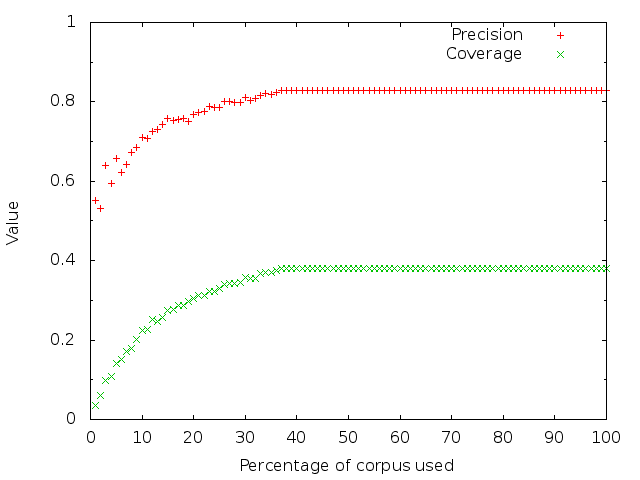
\includegraphics[width=0.45\textwidth]{fig/slot-predicate-percents.png}
    \caption{\label{fig:fonction_predicate}Performance du modèle fonction-prédicat en entraînant le modèle sur une sous-partie du corpus : de 0 à 100~\%.}
\end{figure}

La correspondance probabiliste a une précision 68.33\% mais une couverture
limitée à 38.33\%. La figure~\ref{fig:fonction_predicate} montre que ce niveau
de performance ne demande pas un gros corpus. C'est un enseignement intéressant
pour deux raisons.

\begin{itemize}

    \item Un corpus de petite taille suffit pour obtenir cette performance, ce
    qui est adapté à des domaines où les corpus même non annotés peuvent être
    petits.

    \item L'algorithme ne fait pas de sur-apprentissage en ayant un biais fort
    et une variance faible, ce qui est souhaitable ici.

\end{itemize}

\subsection{Comparaison avec SEMAFOR}

% TODO scores sont en XX
SEMAFOR \citep{das2014frame} est la référence actuelle en annotation en rôles
sémantiques supervisée : c'est le système qui obtient les meilleurs résultats
sur le corpus full-text de FrameNet 1.5. Une comparaison directe n'est pas
possible :

\begin{itemize}
    \item SEMAFOR annote le corpus FrameNet en frames FrameNet et rôles
FrameNet alors que nous l'annotons en classes VerbNet et rôles VerbNet.
    \item Toutes les parties du discours sont annotées alors que nous nous
concentrons sur les verbes.
    \item Les tâches sont découpées différemment. En effet, SEMAFOR découpe la
        tâche en trois parties :
    \begin{itemize}
        \item identification des prédicats déclencheurs ;
        \item identification des frames FrameNet ;
        \item identification des arguments et annotation en rôles sémantiques.
    \end{itemize}
\end{itemize}

Sur la tâche complète, SEMAFOR obtient un score F1 de XX~\%, score à comparer
avec les XX~\% de notre système tout en gardant les limites ci-dessus en tête. 

Il est intéressant de noter l'importance des données d'entraînement pour
SEMAFOR : pour l'identification des frames FrameNet avec des prédicats de la
vérité-terrain\footnote{les résultats pour des déclencheurs identifiés
    manuellement n'ont été donnés que pour le corpus SemEval, un sous-ensemble
du corpus FrameNet 1.5 complet}, les mêmes modèles grimpent de 74.21~\% à
90.51~\% quand la taille du corpus augmente en passant du corpus SemEval (XXX
phrases) au corpus FrameNet 1.5 (XXX phrases).  De la même manière pour
l'identification des arguments avec des frames FrameNet de la vérité-terrain,
les résultats augmentent de 48.09~\% 68.83~\%. C'est très encourageant pour les
domaines disposant de très gros corpus, mais suggère que d'autres solutions
sont à identifier pour les domaines où de tels corpus ne sont pas disponibles.

\section{Travaux futurs}

Nous avons appliqué ce travail à des domaines spécifiques et variés : football,
réchauffement climatique et informatique (Chapitre~\ref{ch:domainsrl}).

% TODO qu'est-ce qui a déjà été fait ici ?
Nous pensons aussi prendre en compte la similarité entre les remplisseurs déjà
identifiés et les remplisseurs pour lesquels un rôle reste encore à identifier
afin d'améliorer nos modèles de probabilité. En effet, l'information des cadres
de sous-catégorisation est cruciale pour identifier les arguments, mais
l'information sémantique concernant le contenu des remplisseurs est aussi utile
pour déterminer le rôle correct.

Enfin, de la même manière que la prise en compte de la voix passive a amélioré
les résultats, d'autres phénomènes de syntaxe profonde doivent être pris en
compte. La coordination est une autre source commune d'erreur. En effet, quand
deux verbes partagent le même sujet, une analyse syntaxique profonde indique à
chaque fois quel est le sujet profond. Voici deux exemples tirés du corpus
FrameNet :

\begin{itemize}

    \item \textit{You are not fair when you belittle Sheik Bin Baz 's blunder and
        exaggerate the one by Sheik Maqdasi ...}

    \item \textit{Hostile and even friendly nations routinely steal information
        from U.S. companies and share it with their own companies}

\end{itemize}

L'objectif est de traiter ces phénomènes de manière plus générale en intégrant
le système de \cite{ribeyre2013systeme} qui permet de prendre en compte de
nouveaux phénomènes en ajoutant de nouvelles règles au système. Ainsi, les
différents phénomènes seront prise en compte de manière cohérente.

\section*{Conclusion}

Nous avons implémenté un système d'annotation en rôles sémantiques basé sur la
connaissance. Nous avons utilisé des outils et des corpus disponibles
publiquement qui rendent notre travail facilement reproductible et facilitent
le travail de comparaison, maintenant et dans le futur. Nous avons commencé à
améliorer le système initial, montrant son potentiel. L'indépendance de
l'approche par rapport au corpus considéré la rend attractive pour annoter des
domaines ne disposant que de peu ou pas de corpus annotés en rôles sémantiques.


% vim: set spelllang=fr:

\setchapterpreamble[ur][\textwidth]{%
  \dictum[Bill Watterson, \textit{Calvin et Hobbes}]{%
    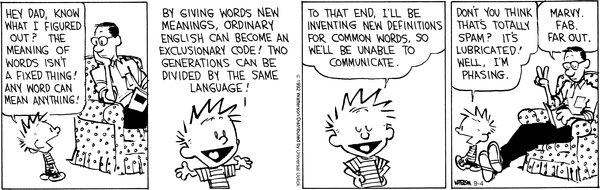
\includegraphics[width=\textwidth]{fig/calvin_meaning.png}}}

\chapter{Annotation en rôle sémantique en domaine spécifique}
\label{ch:domainsrl}

Là où le précédent chapitre présentait notre approche générique d'annotation en
rôles sémantiques fondée sur la connaissance, celui-là cherche à évaluer son
application en domaines spécifiques. À l'heure où les algorithmes supervisés
obtiennent d'excellentes performances sur un certain nombre de tâches quand des
données annotées pour le domaine considéré existent, l'adaptation au domaine
est un défi majeur en Traitement Automatique des Langues, et l'annotation en
rôles sémantiques sur de nouveaux domaines reste un problème ouvert.

Dans ce chapitre, nous n'utilisons pas le système du Chapitre~\ref{ch:srl} et
ne développons pas un système, mais nous évaluons la capacité de VerbNet et
\verbenet{} à traiter des corpus en domaines spécifiques.

La définition du terme 'domaine' reste assez vague dans le sens où il est
difficile de proposer une catégorisation de la connaissance en un ensemble de
domaines qui soit à la fois cohérente et efficace \citep{ma2012rethinking}. Il
est aussi difficile de séparer clairement le «~domaine général~» des domaines
spécifiques. Néanmoins, c'est un phénomène qui existe et qui est à considérer :
les modèles entraînés sur un corpus d'un domaine spécifique (la finance par
exemple) risque de produire des performances mauvaises si appliqués à d'autres
domaines (le football par exemple). C'est le cas par exemple de la
désambiguïsation de classe VerbNet au moment de passer du corpus PropBank à un
corpus du domaine biomédical \citep{abend2008supervised}.

Il est important aussi de différencier le genre et le domaine d'un texte. Le
corpus du Wall Street Journal traite du domaine de la finance dans un genre
journalistique. D'autres genres existent, par exemple les genre littéraires que
sont la fiction, la poésie, le théâtre, etc. Néanmoins, ces distinctions ne
nous concernent pas ici, et l'objectif affiché est de traiter aussi bien un
roman qu'une encyclopédie, un email bien écrit qu'un article de journal.  C'est
une simplification mais les difficultés que nous rencontrons avec les corpus
utilisés dépendent plutôt du domaine que du genre. En effet, nous supposons que
dans deux domaines différents plus que dans deux genres différents, les
changements vont résider dans les verbes utilisés, leur sens et la façon de les
utiliser. C'est ce que nous souhaitons prendre en compte ici.

\section{Corpus considérés}

Afin de s'assurer que notre travail reste valide en changeant de domaine, nous
considérons ici trois corpus présents dans des domaines différents.

\begin{itemize}

    \item le Kicktionary \citep{schmidt2006interfacing,schmidt2009kicktionary}
        rassemblant des dépêches de l'UEFA dans le domaine du football à propos
        de la Ligue Europa, de la Champions League et de la Coupe du Monde. Ce
        corpus est disponible en français, anglais et allemand.

    \item Le DiCoInfo est le corpus Informatique/Internet de l'OLST
        \citep{corpusolst} en anglais, français et espagnol.

    \item Le DiCoEnviro est le corpus Réchauffement climatique de l'OLST
        \citep{corpusolst} en anglais, français et espagnol.

\end{itemize}

Les deux intérêts majeurs communs à ces trois corpus sont :

\begin{enumerate}

    \item de s'inspirer plus ou moins librement de la méthodologie FrameNet, ce
        qui permet d'appliquer nos méthodes,

    \item d'être disponible à la fois en anglais et en français, ce qui permet
        de comparer VerbNet à \verbenet{},

    \item et d'être basés sur l'annotation dans un corpus d'un certain nombre
        de prédicats (ce n'est pas une annotation dite "full-text")

\end{enumerate}

Ce dernier point est plutôt un inconvénient : la manière la plus réaliste de
considérer un corpus d'entraînement est de réaliser une annotation dite
\textit{full-text} en annotant tous les prédicats rencontrés dans un texte
donné. Cependant, les contextes choisis l'ont été à chaque fois sur des
critères de diversité syntaxique
\citep{schmidt2006interfacing,lhomme2012adding}. Le postulat que nous faisons
dans ce travail est que notre méthode est moins affectée par ce problème qu'un
modèle statistique se basant exclusivement sur la distribution des différentes
constructions.

Les trois corpus ont étés découpés en deux parties de tailles égales : un
corpus d'entraînement et un corpus de test. Étant donné qu'il n'y a pas de
modèle à entraîner, ce corpus d'entraînement est simplement utilisé pour
comprendre les erreurs en l'analysant manuellement. Même si les trois corpus
contiennent des textes proches entre eux, ils sont issus de sources différentes
et ont étés écrits par des auteurs différents. Nous avons normalisé ces sources
(par exemple, les sources DEBIAN2 et DEBIAN3 dans le corpus Informatique \&
Internet de l'OLST ont manuellement été transformées verbs DEBIAN) et utilisons
cette information pour faire le découpage : une source spécifique ne peut être
présente que dans un ensemble. Le découpage résultant est disponible au format
JSON avec le code source associé à ce chapitre. Ce découpage ne nécessite pas
d'avoir normalisé les sources : chaque phrase est simplement associée à
l'ensemble de test ou l'ensemble d'entraînement.

\section{Mappings de rôles}

Ces trois corpus utilisent des rôles spécifiques. Les corpus DiCoInfo et
DiCoEnviro utilisent les conventions VerbNet alors que le Kicktionary  définit
un nouvel ensemble de rôles pour chaque frame à la façon de FrameNet, par
exemple \texttt{Passer}, \texttt{Moving\_Ball} ou \texttt{Shot}. Dans les trois
cas, les rôles ne correspondent pas directement aux rôles VerbNet, et il faut
donc établir une correspondance entre les rôles VerbNet et les rôles des trois
corpus.  Nous avons assigné manuellement une classe VerbNet à chaque classe des
trois corpus, tout en faisant correspondre les rôles. Le résultat de ce mapping
est disponible aux URLs suivantes :

\begin{itemize}
    \item DiCoInfo anglais : \url{https://github.com/aymara/knowledgesrl/blob/master/data/domain/info/vnroles_info_en.xml}
    \item DiCoEnviro anglais : \url{https://github.com/aymara/knowledgesrl/blob/master/data/domain/enviro/vnroles_enviro_en.xml}
    \item Kicktionary : \url{https://github.com/aymara/knowledgesrl/blob/master/data/domain/kicktionary/kicktionary-vn-roles.xml}
\end{itemize}

Dans le cas de DiCoInfo et DiCoEnviro, les noms des rôles sont proches des noms
des rôles employés dans VerbNet et LIRICS \citep{bonial2011hierarchical} :
Agent, Patient, Destination, Instrument, etc. Cependant, même si les noms sont
les mêmes, la définition de ces rôles est spécifique à DiCoInfo et DiCoEnviro.
En pratique :

\begin{itemize}

    \item DiCoInfo et DiCoEnviro ne distinguent pas Theme de Patient mais
n'utilisent que Patient, ce qui facilite l'annotation.\footnote{Ce choix est le
bienvenu, étant donné que la distinction entre Theme et Patient est souvent
difficile à établir. Dans \textit{Le chaton a léché mes doigts}, est-ce que mes
doigts ont changé d'état ? Si oui, ils devraient être Patient, et sinon, Theme
\citep[p.~5]{palmer2010semantic}.}

    \item Pour un certain nombre de lexies, la perspective du domaine implique
souvent des rôles différents (TODO exemple Patient vs. Result)

\end{itemize}

Prenons deux phrases d'exemple dans DiCoInfo et DiCoEnviro pour illustrer le
mapping.

\begin{itemize}
    \item \textit{In the interest of fair competition you should ALLOCATE the
        same amount of memory to both engines}.
    \item \textit{Techniques and tools exist to MEASURE carbon stocks in project areas
        relatively precisely depending on the carbon pool.}
\end{itemize}

Dans la première phrase, le sens du verbe \textit{allocate} au sens
\textit{allouer de la mémoire vive} est très précis et très spécifique au domaine
de l'informatique. Pourtant, il se comporte syntaxiquement de la même manière
que le sens plus général considéré par WordNet et OntoNotes: \textit{distribute
or set aside according to plan}. Par conséquent, un mapping manuel a été
réalisé de la lexie allocate.1 (qui correspond à la phrase ci-dessus) vers la
classe VerbNet \textit{future\_having-13.3}. Enfin, les actants définis par
DiCoInfo (qui correspondent aux roles \textit{Core} de FrameNet et aux rôles de
VerbNet) ont étés mis en correspondance avec les rôles de VerbNet :

\begin{itemize}
    \item Patient devient Theme ;
    \item Recipient devient Goal ;
    \item Agent reste Agent.
\end{itemize}

Une fois que ce mapping est réalisé, la tâche de notre algorithme d'annotation
en rôles sémantiques devient de détecter que la classe \texttt{future\_having-13.3} est
utilisée ici, que \textit{You} est Agent, que \textit{the same amount of memory} est Theme,
et que \textit{to both engines} est Goal.

Pour la seconde phrase, la démarche est la même : il s'agit d'identifier que la
classe Verbnet est \texttt{register-54.1}, que \textit{Techniques and tools}
est Agent, et que \textit{carbon stocks} est Theme.

DiCoInfo et DiCoEnviro font une distinction entre les rôles core et non core :
nous n'avons annoté que les rôles core étant donné que VerbNet ne considère que
ces rôles, même si la distinction peut différer entre VerbNet et
DiCoInfo/DiCoEnviro. Étant donné qu'une frame DiCoInfo/DiCoEnviro est un sens
spécifique d'un verbe n'acceptant que des constructions spécifiques, nous avons
toujours associé de tels sens à une seule classe VerbNet.

Le Kicktionary a été plus difficile à associer : ses frames considèrent un
grand nombre de verbes au comportement parfois assez différent. Les règles de
FrameNet indiquent que de telles frames auraient du êtres découpées
\citep{ruppenhofer2006extended}, mais le Kicktionary ne suit pas toujours ces
règles, ayant été développé à part de FrameNet, couvrant un domaine spécifique
au lieu du domaine général, et étant multilingue
\citep{schmidt2006interfacing}. Certaines frames sont définies correctement :
c'est le cas de \texttt{Receive\_Card} et \texttt{Give\_Card} qui correspondent
respectivement à \texttt{obtain-13.5.2} et \texttt{give-13.1-1}. Par contre, la
frame \texttt{Goal} a par exemple été définie pour un but marqué, mais les
différentes façons de l'exprimer n'ont pas étés séparées : ouvrir la marque,
égaliser, frapper, et d'autres utiliseront différentes constructions
syntaxiques, évoqueront des rôles différents et correspondront donc à des
classes VerbNet différentes. Nous n'évaluons pas ces frames.

\if false

\section{Enrichissement de VerbNet}
\label{sec:enrichissement_verbnet}

Malgré leur similarité, ces corpus posent des problèmes différents vis-à-vis de
leur annotation avec VerbNet, tous liés au fait de ne pas être dans le "domaine
général". Nous avons considéré comme problème les manquements dans VerbNet qui
empêchent de prendre en compte les phrases considérées, indépendamment de
l'algorithme. Ainsi, pour que VerbNet puisse prendre en compte une instance, il
faut :

\begin{itemize}
    \item que le sens du verbe considéré soit présent dans VerbNet,
    \item que la construction en question soit présente dans VerbNet,
    \item et que les rôles sémantiques associés à chaque syntagme soient correct.
\end{itemize}

Il y a différentes façons de ne pas respecter ces contraintes dans VerbNet :

\begin{itemize}
    \item Le verbe n'existe pas du tout
    \item Le sens du verbe utilisé n'est pas représenté alors que c'est un sens
        du domaine général
    \item Le sens du verbe utilisé n'est pas représenté alors que c'est un sens
        spécifique à ce domaine
    \item La construction utilisée n'est pas présente
    \item La construction utilisée n'associe pas les arguments aux rôles
        corrects
\end{itemize}

Suivant les corpus considérés, les proportions d'erreurs seront différentes.
Nous avons demandé à deux annotateurs d'évaluer, pour vingt phrases par
domaine, quelle était l'erreur. L'accord inter-annotateur permet de valider la
distinction domaine spécifique/domaine général malgré l'impossibilité de la
définir précisément.

% TODO: le faire....

C'est pour cette raison que l'enrichissement de VerbNet se fait de deux
manières : certains verbes et constructions sont ajoutés comme faisant partie
du domaine général, alors que d'autres sont étiquetés avec le domaine
spécifique correspondant. L'idée est d'éviter que des connaissances de domaines
spécifiques viennent réduire la qualité de la ressource tout en s'assurant que
la couverture de VerbNet pour le domaine général continue de s'améliorer.

\section{Détection semi-automatique d'erreurs}

D'une part, pour minimiser le travail manuel, il est important d'automatiser au
maximum l'enrichissement de la ressource. D'autre part, l'intérêt de VerbNet
réside notamment dans sa capacité à factoriser efficacement ces informations
sur l'interface syntaxico-sémantique d'un verbe donné, et il est donc possible
et utile de valider manuellement chacun des changements apportés.

Le principe suivi est donc d'essayer de détecter les manquements de VerbNet de
manière automatique avant de proposer à un utilisateur expert de réaliser des
changements en ayant un maximum d'informations pertinentes à portée de main.

Les différentes erreurs détectées sont :
\begin{itemize}
    \item l'absence de lemmes dans la ressource
    \item l'absence d'un sens correct dans la ressource
    \item l'absence de constructions correctes dans la ressource
    \item l'absence de mapping de role correct dans la ressource
\end{itemize}

Nous avons d'abord commencé par détecter l'absence de constructions correctes,
ce qui a permis ensuite de détecter une absence de sens en comparant les
constructions observées avec les constructions présentes. Enfin, cela a permis
de faire des propositions quant à la position d'un nouveau lexème dans la
ressource.

% TODO: le faire....

\fi


\section{Comparaison à VerbNet}
\label{comparaison_verbnet}

De simples transformations permettent de gérer l'encodage spécifique de frames
dans DiCoInfo et DiCoEnviro pour l'adapter à VerbNet. Premièrement, des rôles
répétés sont supprimés : \texttt{NP.Agent} \texttt{V} \texttt{NP.Theme}
\texttt{NP.Theme} devient \texttt{NP.Agent} \texttt{V} \texttt{NP.Theme}. En
effet, DiCoInfo et DiCoEnviro répètent le même rôle deux fois quand deux
syntagmes nominaux liés par exemple avec la conjonction «~et~» partagent le
même rôle dans la même frame. Deuxièmement, au moment de rencontrer une forme
\texttt{V} \texttt{NP.Theme}, le syntagme devant le verbe est aussi supprimé
dans VerbNet avant comparaison. Ces formes sont en général des verbes à
l'impératif où le sujet n'est pas exprimé, et doivent dont êtres transformées
avant traitement par VerbNet, VerbNet ne décrivant les frames qu'à l'indicatif.

Dans le cas de \verbenet{}, pour prendre en compte les différences d'encodage
(expliquées à la section~\ref{princp}), nous générons les frames qu'il faut
inférer. Pour ce faire, nous prenons l'ensemble des arguments (syntagmes après
le verbe), et calculons l'ensemble des permutations des parties de cet
ensemble, avec produire des frames complètes à partir de ces permutations.

Pour chaque occurrence de phrase dans notre corpus convertie en rôles VerbNet,
nous :
\begin{itemize}
    \item vérifions si le lemme existe dans VerbNet ou \verbenet{},
    \item observons si la frame syntaxique du corpus est exprimée exactement
        telle quelle dans VerbNet,
    \item regardons si la classe souhaitée d'après le mapping est effectivement
        parmi la liste des classes VerbNet possibles après avoir filtré les
        correspondances syntaxiques,
    \item et déterminons enfin si les rôles sont corrects en considérant la
        classe correcte.
\end{itemize}

Ces quatre observations nous permettent d'évaluer à la fois la couverture de
VerbNet et \verbenet{} (nombre de lemmes présents, nombres de constructions
présentes) mais aussi en terme de précision (est-ce que les rôles sont corrects
?).

La méthode est implémentée dans le dossier \texttt{src/domain} de
\url{https://github.com/aymara/knowledgesrl}.

\section{Résultats}
\label{sec:domainsrlresults}

Nous considérons la couverture de VerbNet dans ces trois ressources, en
mesurant la couverture des lemmes, la couverture des classes, la couverture
syntaxique et l'exactitude des rôles (section~\ref{comparaison_verbnet}). Nous
calculons ces scores sur les occurrences et non pas les types.

\begin{table}[h]
\centering
\begin{tabular}{rccc}
  \toprule
         & Info & Enviro & Kicktionary \\
  \midrule
  Lemme présent          & 80 & 89 & 69 \\
  Frame présente         & 80 & 82 & 69 \\
  Classe correct incluse & 57 & 79 & 11 \\
  Rôle correct           & 94 & 95 & 67 \\
  \bottomrule
\end{tabular}

\caption{\label{table:coverage} Couverture VerbNet en anglais pour les corpus
    DiCoInfo, DiCoEnviro et Kicktionary. Le score de lemme est le pourcentage
    d'occurrences de lemmes verbaux présents dans VerbNet. Le score de frame
    est le pourcentage de correspondances exactes entre les cadres de
    sous-catégorisation VerbNet et cadres identifiés dans les corpus. Le score
    de classe est le pourcentage de classes correctes qui sont présentes
    d'après notre mapping quand la frame était dans VerbNet, indépendemment de
l'ambiguïté. Enfin, le score de rôle est le pourcentage de rôles correctement
identifiés.}

\end{table}

% TODO mapping fini ou non ?
La Table~\ref{table:coverage} présente les résultats pour les trois domaines
considérés. Les résultats du Kicktionary sont à analyser avec prudence : d'une
part, le mapping n'est pas fini, d'où le score de classe extrêmement bas, et
d'autre part aucune analyse d'erreur n'a pour le moment été effectuée. Nous
pouvons tout de même tirer des conclusions de ces résultats.

Premièrement, VerbNet couvre entre 75\% et 84\% des occurrences de lemmes, ce
qui est très encourageant et correspond à notre objectif de couvrir l'ensemble
du vocabulaire.
% TODO couverture FrameNet
Deuxièmement, les résultats varient par domaines : en particulier, le
Kicktionary est le corpus le plus loin de VerbNet. Cependant, les erreurs sont
principalement dues à des mots « du domaine général » qui ne sont pas
spécifiques au football. Par exemple, le verbe \textit{celebrate} est absent du
Kicktionary mais il serait tout de même utile dans le domaine général.
% TODO montrer au-delà d'un exemple (comment ?) que les erreurs dans
% Kicktionary ne sont pas spécifiques et bénéficiraient à VN
%Second, while the results vary between domains, those results are still
%preliminary and the results can change depending on the way frames are encoded
%(the training set of the Kicktionary corpus has not been analyzed yet).
Troisièmement, une fois que la classe a été identifiée correctement, les
résultats sont bons pour les corpus DiCoInfo et DiCoEnviro (plus de 90~\%).

\begin{table}[h]
\centering
\begin{tabular}{rccc}
  \toprule
         & Info & Enviro & Kicktionary \\
  \midrule
  Lemme présent          & 52 & 37 & 42 \\
  Frame présente         & 78 & 84 & 59 \\
  Classe correct incluse & 47 & 46 & 28 \\
  Rôle correct           & 78 & 69 & 68 \\
  \bottomrule
\end{tabular}

\caption{\label{table:coverage} Couverture \verbenet{} en français pour les
corpus DiCoInfo, DiCoEnviro et Kicktionary. \verbenet{} a été développé de
manière complètement indépendante : aucune instruction n'a été donnée pour
obtenir de meilleurs résultat ici, à part de traiter la classe 45, présente
dans beaucoup de cas dans DiCoEnviro.}
\end{table}

De manière attendue, \verbenet{}, encore en développement, a une couverture
plus faible en termes de lemmes présents et de classes incluses, mais les
résultats sont prometteurs. Plus particulièrement, ces résultats seront
l'occasion d'améliorer la couverture de \verbenet{} en utilisant les
informations manquantes pour continuer à améliorer \verbenet{} dans le but de
répondre aux besoins du Traitement Automatique des Langues.

\section*{Conclusion}

Nous avons montré qu'il est possible de réaliser de l'annotation en rôles
sémantique en domaine spécifique en utilisant VerbNet. Le système complet
d'annotation en rôles sémantiques utilisera les techniques décrites au
Chapitre~\ref{ch:srl}.

Notre approche rend possible l'annotation d'un nouveau domaine avant de passer
à une annotation manuelle. Il est aussi possible de l'utiliser comme une simple
baseline contre des approches plus sophistiquées. Enfin, utiliser cet outil sur
de nouveaux domaines est un moyen efficace d'obtenir de meilleures performances
mais aussi de guider de nouveaux développements VerbNet étant donné que les
lemmes, classes et frames manquants sont montrées.


\section*{Remerciements}

Merci à Marie-Claude L'Homme et Thomas Schmidt pour nous avoir fournis les
corpus DiCoInfo, DiCoEnviro et Kicktionary.


\chapter*{Conclusion}
\label{ch:conc}

\section{Perspectives}

broad-coverage semantic parsing
FrameNet more syntax stuff, eg. light verbs et je sais pas quoi baker2014framenet yang2014multi

\backmatter
% A glossary and list of acronyms may go here
% or may go in the front matter after the abstract.

\bibliographystyle{plainnat}
\bibliography{bibtex-file/bib}

\part{Annexes}

\chapter{Reproduction des systèmes utilisés}

Ce chapitre traite de divers détails destinés à aider le lecteur a reproduire
un des systèmes présentés dans ces travaux.

\section{Relations syntaxiques identifiées par LIMA présentes dans notre modèle
de langue syntaxique}
\label{relations_modele_langue}

Cette table décrit les identifiants des relations syntaxiques utilisés dans
LIMA et donc présents dans le modèle de langue syntaxique que nous utilisons
pour traduire WordNet. Ces relations ont été définies à partir des relations
définies lors des campagnes d'évaluation Easy et Passage. La définition
initiale d'un certain nombre d'entre elles se trouve dans le guide d'annotation
de la campagne Easy
(\url{http://perso.limsi.fr/Individu/anne/Guide/PEAS_reference_annotations_v2.2.html}).
Il faut noter que dans ces campagnes les relations sont indiquées entre
constituants, alors que LIMA fournit des relations en dépendances (les
relations sont alors entre les têtes des syntagmes correspondants).

\begin{longtable}{lll}
    \toprule
    Identifiant   & Description & Exemples fréquents \\ \midrule
    ADJPRENSUB    &  adjectif épithète pré-nominal         & premier fois, présent loi, bon état \\ \midrule
    ADVADJ        &  adverbe modifiant un adjectif         & tout autre, plus grand \\ \midrule
    ADVADV        &  adverbe modifiant un adverbe          & tout simplement, très bien \\ \midrule
    AdvSub        &  adverbe modifiant un substantif       & que j, beaucoup plus, non pas \\ \midrule
    AdvVerbe      &  adverbe modifiant un verbe            & haut voir, ici envoyer \\ \midrule
    APPOS         &  apposition (cf. APP dans PEAS)        & aristocrate royaliste, abri piscine \\ \midrule
    ATB\_O        &  \specialcell{attribut de l'objet (cf. ATB\_SO \\ dans PEAS)} & site site, álbum annuaire \\ \midrule
    ATB\_S        &  \specialcell{attribut du sujet en relation avec le \\ verbe (cf. ATB\_SO dans PEAS)} & disponible être, possible être \\ \midrule
    ATB\_SG       &  \specialcell{attribut du sujet en relation avec le \\ sujet} & nouveau message \\ \midrule
    COD\_V        &  complément d'objet direct du verbe    & être pouvoir,  profil voir \\ \midrule
    COMPADJ       &  complément de l'adjectif              & site plan, page haut \\ \midrule
    COMPADV       &  complément de l'adverbe               & page haut, forum uniquement \\ \midrule
    COMPDUNOM     &  complément du nom                     & page numéro, page pas, page haut \\ \midrule
    COMPL         &  \specialcell{complémenteur (cf. COMP dans \\ PEAS)} & que être, que avoir, si être \\ \midrule
    CPL\_V        &  \specialcell{complément indirect ou \\ circonstanciel du verbe } & être être, être avoir  \\ \midrule
    CPLV\_V       &  \specialcell{groupe prépositionnel infinitif après \\ le verbe} & connecter cliquer, voir revenir \\ \midrule
    DetIntSub     &  déterminant interrogatif              & quelle période, quelle manière \\ \midrule
    DetSubNum     &  déterminant numéral cardinal          & neuf appartement, trente an \\ \midrule
    MOD\_A        &  modificateur de l'adjectif            & être vrai, être même, être autre \\ \midrule
    MOD\_N        &  modificateur du nom                   & commander libraire, être personne  \\ \midrule
    MOD\_V        &  modificateur du verbe                 & que être, être aller, matière tabler \\ \midrule
    NePas         &  négation                              & ne pas, ne rien, ne jamais \\ \midrule
    Prefixe       &  préfixe                               & il- pas, il- être, anti-criminalité \\ \midrule
    PrepDetInt    &  \specialcell{relation entre préposition et \\ déterminant interrogatif} & de quelle, dans quelle, pour quelle \\ \midrule
    PrepPronCliv  &  \specialcell{relation entre préposition et \\ conjonction de subordination \\ considérée comme un pronom clivé} & de que, em que, une que \\ \midrule
    PrepPron      &  \specialcell{relation entre préposition et \\ pronom personnel} & de tézigue, pour mézigue \\ \midrule
    PrepPronRelCa &  \specialcell{relation entre préposition et pronom \\ relatif complément d'attribution} & dans lequel, pour qui, sur lequel  \\ \midrule
    PrepPronRel   &  \specialcell{relation entre préposition et pronom \\ relatif} & de quoi, en quoi, comme quoi \\ \midrule
    SUBADJPOST    &  adjectif épithète post-nominal        & posté profil, référencé page \\ \midrule
    SUBSUBJUX     &  substantif juxtaposé à un substantif  & top thé, article présent, web site \\ \midrule
    SUJ\_V        &  sujet du verbe                        & j avoir, thé pager, j être \\ \midrule
    SUJ\_V\_REL   &  \specialcell{pronom sujet du verbe de la \\ proposition relative} & qui être, que avoir \\ \midrule
    SUJ\_V\_RELG  &  \specialcell{antécédent sujet du verbe de la \\ proposition relative} & définition suivre, personne avoir \\
    \bottomrule

    \caption{\label{table:relationswonef}Relations syntaxiques présentes dans
        le modèle de langue syntaxique utilisé pour la traduction de WordNet
        vers WoNeF. La troisième colonne présente plusieurs exemples de
        relations entres lemmes fréquentes dans les corpus. Le modèle de langue
    est disponible sur \protect\url{http://www.kalisteo.fr/demo/semanticmap/}.}
\end{longtable}



\section{Sélecteurs employés pour produire WoNeF}
\label{selecteurs_wonef}

\subsection{Combinaisons de sélecteurs initiaux}

\begin{table}[ht]
    \centering
    \begin{tabular}{lll}
        \toprule
        Noms &  haute précision &  monosémie, unicité, Levenshtein \\
        Noms &  haut F-score    &  monosémie, unicité, sources multiples, Levenshtein \\
        Noms &  haute couverture  &  monosémie, unicité, sources multiples, Levenshtein \\
        \midrule
        Verbes &  haute précision &  unicité \\
        Verbes &  haut F-score    &  unicité, monosémie \\
        Verbes &  haute couverture  &  monosémie, unicité, sources multiples \\
        \midrule
        Adjectifs  &  haute précision &  monosémie, unicité, Levenshtein \\
        Adjectifs  &  haut F-score    &  monosémie, unicité, sources multiples, Levenshtein \\
        Adjectifs  &  haute couverture  &  monosémie, unicité, sources multiples, Levenshtein \\
        \midrule
        Adverbes  &  haute précision &  monosémie, unicité, sources multiples, Levenshtein \\
        Adverbes  &  haut F-score    &  monosémie, unicité, sources multiples, Levenshtein \\
        Adverbes  &  haute couverture  &  monosémie, unicité, sources multiples, Levenshtein \\
        \bottomrule
    \end{tabular}
    \caption{Combinaison de sélecteurs initiaux utilisée pour chaque couple
    (partie du discours, version de WoNeF). Ces sélecteurs sont décrits aux
sections~\ref{jaws_extraction_heuristics} et
\ref{subsec:revisiting_extraction_heuristics}.}
\end{table}

\subsection{Combinaisons de sélecteurs syntaxiques}

\cite[section 3.1.1.3]{mouton2010phd} décrit les sélecteurs syntaxiques
utilisés dans WoNeF. Les relations utilisées sont décrites à la
section~\ref{relations_modele_langue}.

\begin{itemize}
    \item Le seul sélecteur syntaxique utilisé pour les verbes, adjectifs et
        adverbes est le sélecteur par synonymie avec diverses relations
        syntaxiques pouvant refléter la synonymie. Par exemple, avec la
        relation COD\_V inverse, on exprime le fait que les verbes qui acceptent
        les mêmes objets sont potentiellement synonymes.
        \begin{itemize}
            \item Les verbes utilisent les relations COD\_V inverse, CPL\_V
                inverse et CPLV\_V inverse.
            \item Les adjectifs utilisent les relations SUBADJPOST ADVADJ
                inverse, et et ATBSG.
            \item Les adverbes utilisent les relations AdvSub inverse et ADVADJ
                inverse.
        \end{itemize}
    \item Concernant les noms, la configuration change suivant la version de WoNeF.
        \begin{itemize}
            \item La version haute précision utilise les sélecteurs de
                méronymie avec la relation COMPDUNOM
                (Figure~\ref{meronymyexample}) et d'holonymie avec la relation
                COMPDUNOM inverse.
            \item La version à haut F-score rajoute le sélecteur par
                hyperonymie avec la relation syntaxique COD.
            \item La version à haute couverture rajoute elle les sélecteurs
                par synonymie (COMPDUNOM, COD\_V et APPOS), hyperonymie
                (COMPDUNOM et SUJ\_V) et hyponymie (COMPDUNOM).
        \end{itemize}
\end{itemize}

\section{Règles d'identification des arguments}
\label{argument_identification}

Les symboles $\uparrow$ et $\downarrow$ indiquent la direction de la
dépendance.

Les relations de la deuxième règle sont IM$\uparrow\downarrow$,
PRT$\downarrow$, COORD$\uparrow\downarrow$, P$\uparrow\downarrow$,
OBJ$\uparrow$, PMOD$\uparrow$, ADV$\uparrow$, SUB$\uparrow\downarrow$,
ROOT$\uparrow$, TMP$\uparrow$, SBJ$\uparrow$ et OPRD$\uparrow$.

Les relations de la quatrième règle sont ADV$\uparrow\downarrow$,
AMOD$\uparrow\downarrow$, APPO$\uparrow\downarrow$, BNF$\uparrow\downarrow$-,
CONJ$\uparrow\downarrow$, COORD$\uparrow\downarrow$, DIR$\uparrow\downarrow$,
DTV$\uparrow\downarrow$-, EXT$\uparrow\downarrow$-, EXTR$\uparrow\downarrow$,
HMOD$\uparrow\downarrow$, IOBJ$\uparrow\downarrow$, LGS$\uparrow\downarrow$,
LOC$\uparrow\downarrow$, MNR$\uparrow\downarrow$, NMOD$\uparrow\downarrow$,
OBJ$\uparrow\downarrow$, OPRD$\uparrow\downarrow$, POSTHON$\uparrow\downarrow$,
PRD$\uparrow\downarrow$, PRN$\uparrow\downarrow$, PRP$\uparrow\downarrow$,
PRT$\uparrow\downarrow$, PUT$\uparrow\downarrow$, SBJ$\uparrow\downarrow$,
SUB$\uparrow\downarrow$ et SUFFIX$\uparrow\downarrow$.

\chapter{Liste des publications}

Quentin Pradet, Jeanne Baguenier-Desormeaux, Gaël de Chalendar et Laurence Danlos. Juin 2013. WoNeF : amélioration, extension et évaluation d’une traduction française automatique de WordNet. TALN 2013, Les Sables d'Olonne, France.

Quentin Pradet, Gaël de Chalendar and Guilhem Pujol. December 2013. Revisiting knowledge-based Semantic Role Labeling. LTC'13, Poznań, Poland.

Quentin Pradet, Gaël de Chalendar and Jeanne Baguenier Desormeaux. January 2014. WoNeF, an improved, expanded and evaluated automatic French translation of WordNet. GWC 2014, Tartu, Estonia.

Quentin Pradet, Laurence Danlos and Gaël de Chalendar. May 2014. Adapting VerbNet to French using existing resources. LREC 2014, Reykjavik, Iceland.

Laurence Danlos, Takuya Nakamura and Quentin Pradet. July 2014. Vers la création d’un Verb$\ni$Net du français. Atelier FondamenTAL, TALN 2014, Marseille, France.


%\chapter{Glossaire}
%Un certain nombre de termes utilisés par la communauté scientifique ne sont pas
%encore parfaitement établis : ce glossaire a pour objet de définir avec
%précision les termes utilisés dans ces travaux. L'objectif étant d'aller vers
%une standardisation, nous nous sommes efforcé d'utiliser les sens les plus
%communs dès que c'était possible.
%\printglossary


\end{document}
